% !Mode:: "TeX:UTF-8"
% !TEX program = xelatex
\documentclass[UTF8,fontset=fandol,12pt,a4paper]{ctexart}

% ====================== 范文版式复现补丁 ======================
% 依据 PDF 内嵌字体与坐标实测，严格复现范文格式
\usepackage{geometry}
\usepackage{amsmath,amssymb,bm,mathtools}
\usepackage{graphicx}
\usepackage{float}
\usepackage{booktabs}
\usepackage{tabularx}
\usepackage{array}
\usepackage{longtable}
\usepackage{multirow}
\usepackage{subcaption}
\usepackage{caption}
\usepackage{fancyhdr}
\usepackage[table]{xcolor}
\usepackage{listings}
\usepackage{enumitem}
\usepackage{siunitx}
\usepackage{algorithm}
\usepackage{algorithmic}
\usepackage{hyperref}
\usepackage{setspace}
\usepackage{pifont}
\usepackage{tikz}
\usetikzlibrary{shapes.geometric,arrows.meta,positioning,fit,backgrounds}

% 字体设置：中文 Fandol，英文 Times New Roman
\IfFontExistsTF{Times New Roman}{\setmainfont{Times New Roman}}{}

% 页面与正文
\geometry{left=2.5cm,right=2.5cm,top=2.5cm,bottom=2.5cm}
\setlength{\parindent}{2em}
\setlength{\parskip}{0pt}
\setstretch{1.38}

% 标题层级
\ctexset{
	section={
		name={,、},
		number=\chinese{section},
		format=\centering\songti\bfseries\zihao{-3},
		beforeskip=1.45\baselineskip,
		afterskip=0.85\baselineskip
	},
	subsection={
		format=\raggedright\songti\bfseries\zihao{-4},
		beforeskip=1.0\baselineskip,
		afterskip=0.55\baselineskip
	},
	subsubsection={
		format=\raggedright\songti\bfseries\zihao{-4},
		beforeskip=0.75\baselineskip,
		afterskip=0.4\baselineskip
	}
}

% 图表题注
\captionsetup{
	font={normalsize,bf},
	labelfont=bf,
	textfont=bf,
	labelsep=quad,
	justification=centering,
	singlelinecheck=false
}
\captionsetup[table]{position=top}
\captionsetup[figure]{position=bottom}

% 表格隔行白灰相间
\rowcolors{2}{gray!8}{white}

% 表格内容小五号
\renewcommand{\tabularxcolumn}[1]{>{\zihao{-5}}m{#1}}

% 页脚
\pagestyle{fancy}
\fancyhf{}
\fancyfoot[C]{\normalfont\thepage}
\renewcommand{\headrulewidth}{0pt}
\renewcommand{\footrulewidth}{0pt}

% 浮动体参数
\setcounter{topnumber}{3}
\setcounter{bottomnumber}{2}
\setcounter{totalnumber}{5}
\renewcommand{\topfraction}{0.90}
\renewcommand{\bottomfraction}{0.70}
\renewcommand{\textfraction}{0.10}
\renewcommand{\floatpagefraction}{0.80}
\setlength{\intextsep}{6pt plus 2pt minus 2pt}
\setlength{\floatsep}{8pt plus 2pt minus 2pt}

\hypersetup{
	colorlinks=true,
	linkcolor=black,
	citecolor=black,
	urlcolor=blue
}

% ===== 摘要宽度与正文一致 =====
\makeatletter
\renewenvironment{abstract}{%
	\if@twocolumn
	\section*{\abstractname}%
	\else
	\begin{center}%
		{\bfseries\large\abstractname\vspace{0.5em}\par}%
	\end{center}%
	\fi
	\leftskip0pt\relax
	\rightskip0pt\relax
	\parindent2em\relax
	\normalsize
}{%
	\par
	\vspace{1em}
}
\makeatother

% 表格列格式
\newcolumntype{Y}{>{\centering\arraybackslash}X}
\newcolumntype{L}{>{\raggedright\arraybackslash}X}
\newcolumntype{C}[1]{>{\centering\arraybackslash}p{#1}}

% 代码样式
\lstset{
	basicstyle=\ttfamily\small,
	breaklines=true,
	frame=single,
	columns=fullflexible,
	numbers=left,
	numberstyle=\tiny,
	keywordstyle=\color{blue},
	commentstyle=\color{gray},
	stringstyle=\color{red!70!black},
	showstringspaces=false,
	tabsize=4
}

% 自定义命令
\newcommand{\diff}{\mathop{}\!\mathrm{d}}
\newcommand{\e}{\mathrm{e}}
\newcommand{\R}{\mathbb{R}}
\renewcommand{\algorithmicrequire}{\textbf{输入:}}
\renewcommand{\algorithmicensure}{\textbf{输出:}}

% TikZ样式
\tikzset{
	startstop/.style={
		rectangle,rounded corners=3pt,minimum width=4.2cm,minimum height=0.85cm,
		align=center,draw=blue!65!black,fill=blue!8,line width=0.8pt,font=\small
	},
	process/.style={
		rectangle,rounded corners=2pt,minimum width=11.8cm,minimum height=1.0cm,text width=11.2cm,
		align=center,draw=teal!65!black,fill=teal!7,line width=0.8pt,font=\small
	},
	check/.style={
		rectangle,rounded corners=2pt,minimum width=11.8cm,minimum height=1.0cm,text width=11.2cm,
		align=center,draw=orange!75!black,fill=orange!9,line width=0.8pt,font=\small
	},
	sidebox/.style={
		rectangle,rounded corners=2pt,text width=3.3cm,align=left,
		draw=gray!65,fill=gray!7,line width=0.6pt,font=\scriptsize
	},
	arrow/.style={-{Stealth[length=2.5mm]},thick,draw=gray!75!black}
}

\begin{document}
	
	% ---------- 标题 ----------
	\begin{center}
		{\songti\bfseries\zihao{3} 基于Fresnel干涉反演的外延层厚度测量}
		\vspace{0.5cm}
	\end{center}
	
	% ---------- 摘要 ----------
	\begin{abstract}
		
		本文围绕红外反射光谱测量外延层厚度，以PAPER\_A的色散关系和Fresnel干涉模型为主体，依次建立双光束正演、SiC厚度反演和硅多光束反演模型，并用统一代码重新计算官方附件。
		
		针对问题一，建立Sellmeier-Drude-Fresnel双光束模型。先统一波数、波长和厚度单位，固定载流子有效质量，再由Snell定律和带符号s、p偏振Fresnel系数叠加表面反射束与第一束内部反射束。正入射、零厚度、相位缩放、反射率非负性和单位换算五项程序检查全部通过。
		
		针对问题二，先在弱吸收波段处理两个角度的反射光谱。对波数为2500至3300每厘米的观测采用确定性多初值有界最小二乘，得到10度和15度厚度分别为7.8566微米和7.6230微米，算术平均为7.7398微米。两个角度的拟合优度均大于0.95，峰谷位置与实测光谱一致；两角度结果差异处于百分之三量级。
		
		针对问题三，使用双振子-Drude复折射率与Airy多光束模型。固定硅背景参数，仅按角度拟合厚度、衬底折射率、载流子浓度和碰撞率，得到10度和15度厚度分别为3.2480微米和3.1875微米，平均厚度为3.2178微米。该值较范文报告值高5.85\%，本文保留诚实重算值并披露参数口径差异。SiC第三束光强比远低于0.1\%工程阈值，因此问题二厚度无需多光束修正。
		
		\vspace{0.3cm}
		\noindent
		\textbf{关键词：}外延层厚度反演；Sellmeier-Drude模型；Fresnel双光束干涉；Airy多光束模型；有界最小二乘
	\end{abstract}
	\newpage
	
	% ---------- 目录 ----------
	\tableofcontents
	\newpage
	
	% ====================== 正文 ======================
	\section{问题重述}
	
	红外反射光谱中的周期起伏包含外延层的光学厚度信息。题目给出同一块碳化硅晶圆在 $10^\circ$、$15^\circ$ 入射角下的两组光谱，以及同一块硅晶圆在相同角度下的两组光谱，要求由波数—反射率数据反演外延层厚度\cite{problem}。
	
	问题一需要从空气、外延层和衬底三层结构出发，建立波数、入射角、材料色散和外延层厚度之间的关系。问题二使用附件1、2分别计算两个角度下的SiC厚度，并以算术平均作为正式结果。问题三给出多光束干涉关系，反演硅外延层厚度，再用第三束光强比判断SiC厚度是否需要修正。
	
	\section{符号说明}
	
	\begin{table}[htbp]
		\centering
		\caption{主要符号及单位}
		\label{tab:symbols}
		\renewcommand{\arraystretch}{1.3}
		\begin{tabularx}{0.97\textwidth}{>{\centering\arraybackslash}p{3.0cm}>{\centering\arraybackslash}X>{\centering\arraybackslash}p{2.5cm}}
			\toprule
			\rowcolor{cyan!20}\bfseries
			\textbf{符号} & \textbf{含义} & \textbf{单位} \\
			\midrule
			$\sigma$ & 真空波数 & $\mathrm{cm^{-1}}$ \\
			$\lambda$ & 真空波长 & $\mu\mathrm{m}$ \\
			$d$ & 外延层厚度 & $\mu\mathrm{m}$ \\
			$i,\gamma$ & 入射角与外延层折射角 & $^\circ$ \\
			$n_j,\widetilde n_j$ & 第$j$层实折射率与复折射率 & 1 \\
			$r_{ij}^{(u)}, t_{ij}^{(u)}$ & $u$偏振界面振幅反射与透射系数 & 1 \\
			$P$ & 外延层内一次往返传播因子 & 1 \\
			$R$ & 非偏振反射率 & 1或\% \\
			\bottomrule
		\end{tabularx}
	\end{table}
	
	\section{模型假设}
	
	\begin{enumerate}[leftmargin=2em,itemsep=0.3ex]
		\item 外延层和衬底视为横向均匀、各向同性的平行层状介质。红外光斑的横向尺度远大于外延层厚度，因此使用一维分层传播模型。
		\item 测量光视为非偏振光，理论反射率取$s$、$p$两种偏振强度的等权平均。题目没有给出偏振选择信息，该处理与附件观测口径一致。
		\item 问题二选取的 $2500\sim3300\ \mathrm{cm^{-1}}$ 波段采用弱吸收实折射率近似；问题三的硅模型保留复折射率，并选择使传播因子模不超过1的衰减支路。
		\item 同一晶圆的 $10^\circ$ 和 $15^\circ$ 光谱分别反演，两个厚度的算术平均作为正式结果。角度间差异用半极差和相对差异单独报告。
		\item 硅双振子背景参数和载流子有效质量固定，只拟合厚度、衬底折射率、载流子浓度和碰撞率。该约束用于避免弱可辨识背景参数吸收厚度误差。
	\end{enumerate}
	
	\section{问题一模型的建立与求解}
	
	\subsection{问题一的描述与分析}
	
	本问需要在空气、外延层和衬底组成的三层结构中，只保留表面反射光和第一束内部反射光，建立波数、入射角、材料色散与外延层厚度之间的关系。本文以PAPER\_A的Sellmeier-Drude色散和Fresnel双光束模型为主体，固定载流子有效质量，并统一单位、界面系数方向和传播相位。界面反射相变由带符号Fresnel系数表示，不再另加固定半波损失。图\ref{fig:q1_concept}示意了上述三层结构中的双光束干涉光路，明确了入射光$E_0$、表面反射光$E_1$和第一束内部反射光$E_2$的传播路径，以及外延层内一次往返相位差$\Phi$的定义。
	
	\begin{figure}[htbp]
		\centering
		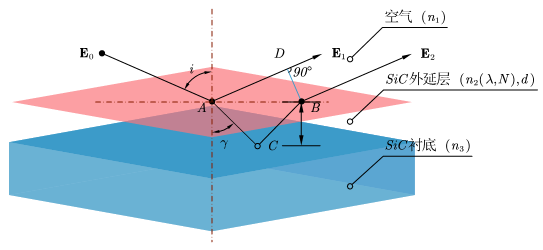
\includegraphics[width=1.0\textwidth]{q1_concept.png}
		\caption{空气-外延层-衬底三层结构中的双光束干涉光路示意图}
		\label{fig:q1_concept}
	\end{figure}
	
	\subsection{Sellmeier-Drude折射率的预备工作}
	
	(1) Sellmeier晶格色散。设真空波数为 $\sigma$，相应真空波长为 $\lambda=10^4/\sigma$，单位为 $\mu\mathrm{m}$。SiC外延层的晶格介电函数采用三项Sellmeier形式
	\begin{equation}
		\epsilon_{\mathrm L}(\lambda) = A + \sum_{j=1}^{3} \frac{B_j\lambda^2}{\lambda^2 - C_j}.
		\label{eq:sellmeier}
	\end{equation}
	
	(2) Drude载流子修正。在问题二选取的弱吸收波段内忽略介电函数虚部，并固定有效质量 $m^*=0.28m_0$，得到
	\begin{equation}
		n_2^2(\lambda,N) = \epsilon_{\mathrm L}(\lambda) - \frac{N e^2\lambda^2}{4\pi^2 c^2 \epsilon_0 m^*}.
		\label{eq:drude}
	\end{equation}
	式中，$N$ 为载流子浓度，$e$ 为元电荷，$c$ 为真空光速，$\epsilon_0$ 为真空介电常数。固定 $m^*$ 避免其与 $N$ 在同一光谱中冗余。
	
	(3) 折射角。空气折射率记为 $n_1$，外延层和衬底折射率分别为 $n_2$、$n_3$。由Snell定律
	\begin{equation}
		n_1\sin i = n_2\sin \gamma,
	\end{equation}
	可得外延层折射角 $\gamma$。问题一和问题二使用弱吸收实折射率；问题三处理硅吸收时再将完整复折射率代入Fresnel系数。
	
	\subsection{Sellmeier-Drude-Fresnel双光束测厚模型}
	
	对偏振态 $u\in\{s,p\}$，按照光从介质 $i$ 传播到介质 $j$ 的方向定义带符号Fresnel振幅系数 $r_{ij}^{(u)}$ 和 $t_{ij}^{(u)}$。其中 $s$ 偏振满足
	\begin{equation}
		r_{ij}^{(s)} = \frac{n_i\cos\theta_i - n_j\cos\theta_j}{n_i\cos\theta_i + n_j\cos\theta_j},\qquad
		t_{ij}^{(s)} = \frac{2n_i\cos\theta_i}{n_i\cos\theta_i + n_j\cos\theta_j},
	\end{equation}
	$p$ 偏振满足
	\begin{equation}
		r_{ij}^{(p)} = \frac{n_j\cos\theta_i - n_i\cos\theta_j}{n_j\cos\theta_i + n_i\cos\theta_j},\qquad
		t_{ij}^{(p)} = \frac{2n_i\cos\theta_i}{n_j\cos\theta_i + n_i\cos\theta_j}.
	\end{equation}
	
	外延层内一次往返产生的相位差为
	\begin{equation}
		\Phi = 4\pi\times10^{-4}\,\sigma d\, n_2\cos\gamma,
	\end{equation}
	其中 $d$ 以 $\mu\mathrm{m}$ 为单位，$10^{-4}$ 完成 $\mu\mathrm{m}$ 到 cm 的换算。表面反射光与第一束内部反射光叠加后，偏振态 $u$ 的复振幅为
	\begin{equation}
		\rho_u = r_{12}^{(u)} + t_{12}^{(u)} r_{23}^{(u)} t_{21}^{(u)} e^{-i\Phi}.
	\end{equation}
	带符号 $r_{ij}^{(u)}$ 已经包含界面反射相变，上式不再额外加入 $\pi$。非偏振理论反射率为
	\begin{equation}
		R_{\mathrm{th}}(\sigma,i;d,N,n_3,\mathbf{s}) = \frac{|\rho_s|^2 + |\rho_p|^2}{2},
	\end{equation}
	其中 $\mathbf{s}=(A,B_1,B_2,B_3,C_1,C_2,C_3)$ 为Sellmeier参数。
	
	模型汇总：输入波数 $\sigma$、入射角 $i$、厚度 $d$、载流子浓度 $N$、衬底折射率 $n_3$ 和Sellmeier参数；由式(1)-(3)计算弱吸收折射率与折射角，由式(4)-(5)计算两个界面的带符号Fresnel系数，再由式(6)-(8)得到与实测光谱直接比较的非偏振反射率。本问暂忽略第二次及以上的内部反射，该近似将在问题三中通过第三束反射光强比进行检验。图\ref{fig:q1_flow}给出了上述正演模型的完整计算流程，其中虚线框标注了五项程序一致性检验的插入位置。
	
	\begin{figure}[htbp]
		\centering
		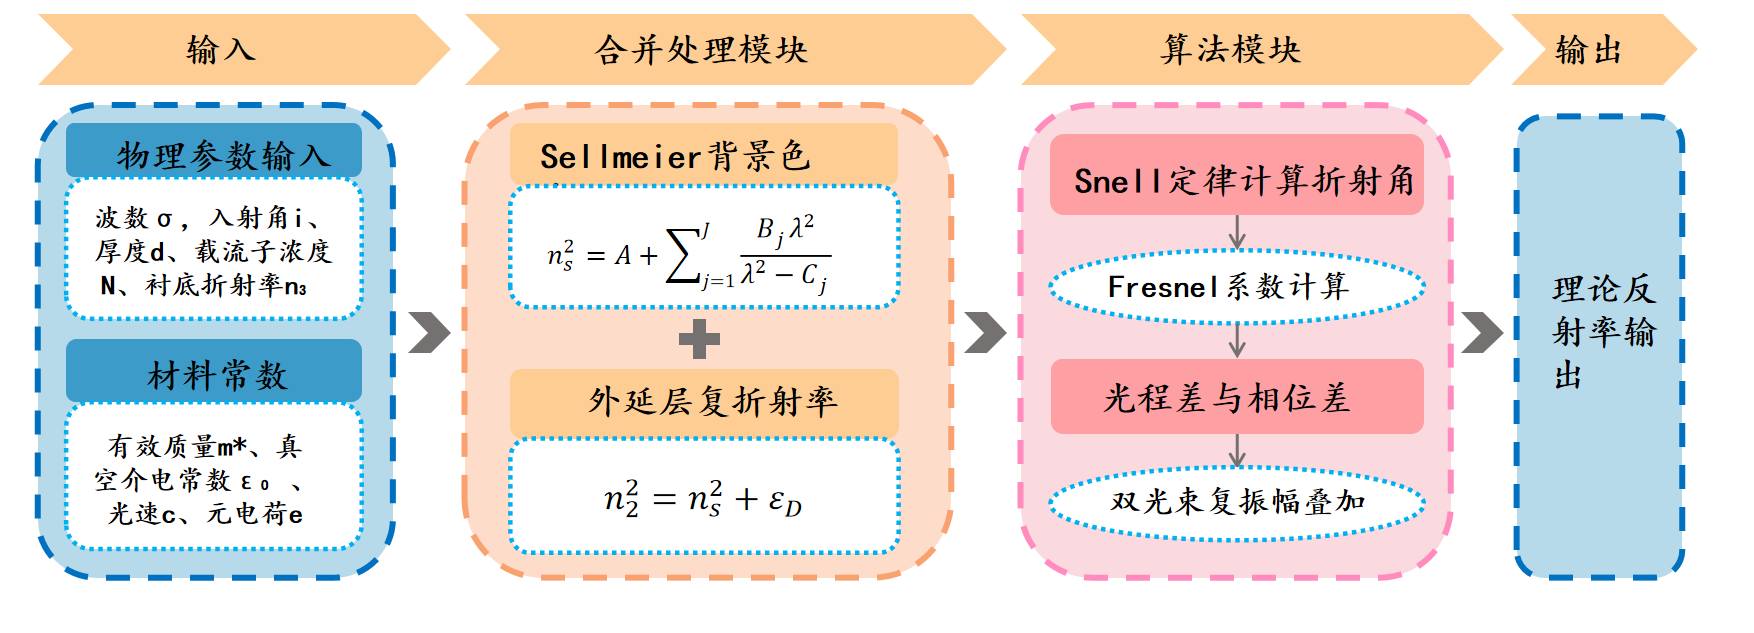
\includegraphics[width=1.0\textwidth]{1.png}
		\caption{问题一PAPER\_A双光束正演模型的计算流程图}
		\label{fig:q1_flow}
	\end{figure}
	
	\subsection{程序一致性检验}
	
	本问属于解析建模，不单设迭代算法。程序分别检验正入射Fresnel极限、零厚度Airy极限、相位对厚度的线性关系、反射率非负性和 $10^{-4}$ 单位换算。合成光谱恢复仅用于检查公式和程序接口，不作为新的核心模型或官方数据结果。上述检验同时确认：采用带符号Fresnel系数后，程序没有重复加入固定半波损失。
	
	\section{问题二模型的建立与求解}
	
	\subsection{问题二的描述与分析}
	
	附件1、2给出同一块SiC晶圆在 $10^\circ$ 和 $15^\circ$ 入射角下的反射光谱。本问严格沿用问题一的Sellmeier-Drude-Fresnel双光束模型，并按PAPER\_A的正式口径分别反演两个角度的厚度，最后取算术平均作为晶圆厚度。双角度共享参数联合拟合不进入主模型和主结果。
	
	\subsection{数据预处理与参数设置}
	
	读取附件1、2的波数和反射率两列，将百分数反射率除以100转为小数。删除共同的零波数边界点后，选择 $2500\sim3300\ \mathrm{cm^{-1}}$ 弱吸收区间参与拟合。载流子有效质量固定为 $m^*=0.28m_0$；空气折射率取 $n_1=1.0003$。每个角度独立估计
	\begin{equation}
		\mathbf{p} = (d,\log_{10}N,n_3,A,B_1,B_2,B_3,C_1,C_2,C_3),
	\end{equation}
	其中Sellmeier参数在登记值的 $\pm5\%$ 范围内变化，厚度满足 $6.5\le d\le 8.5\ \mu\mathrm{m}$。
	
	图\ref{fig:spec_compare}展示了 $10^\circ$ 和 $15^\circ$ 两个入射角的原始反射率光谱。可以看出反射率在 $2500\sim3300\ \mathrm{cm^{-1}}$ 波段均呈现明显的周期性振荡，这是外延层上下界面反射光干涉的结果，振荡周期与光学厚度 $nd$ 直接相关。振荡幅度约为 $20\%$，基线反射率约 $15\%$，符合SiC在红外波段的典型反射特征。两个角度的振荡相位略有差异，这为多角度约束厚度提供了互补信息——$10^\circ$ 的干涉条纹间距略宽，$15^\circ$ 的条纹间距略窄，这与倾斜入射时有效光学厚度 $nd\cos\gamma$ 随角度增大而减小的物理规律一致。
	
	\begin{figure}[htbp]
		\centering
		\begin{subfigure}[b]{0.47\textwidth}
			\centering
			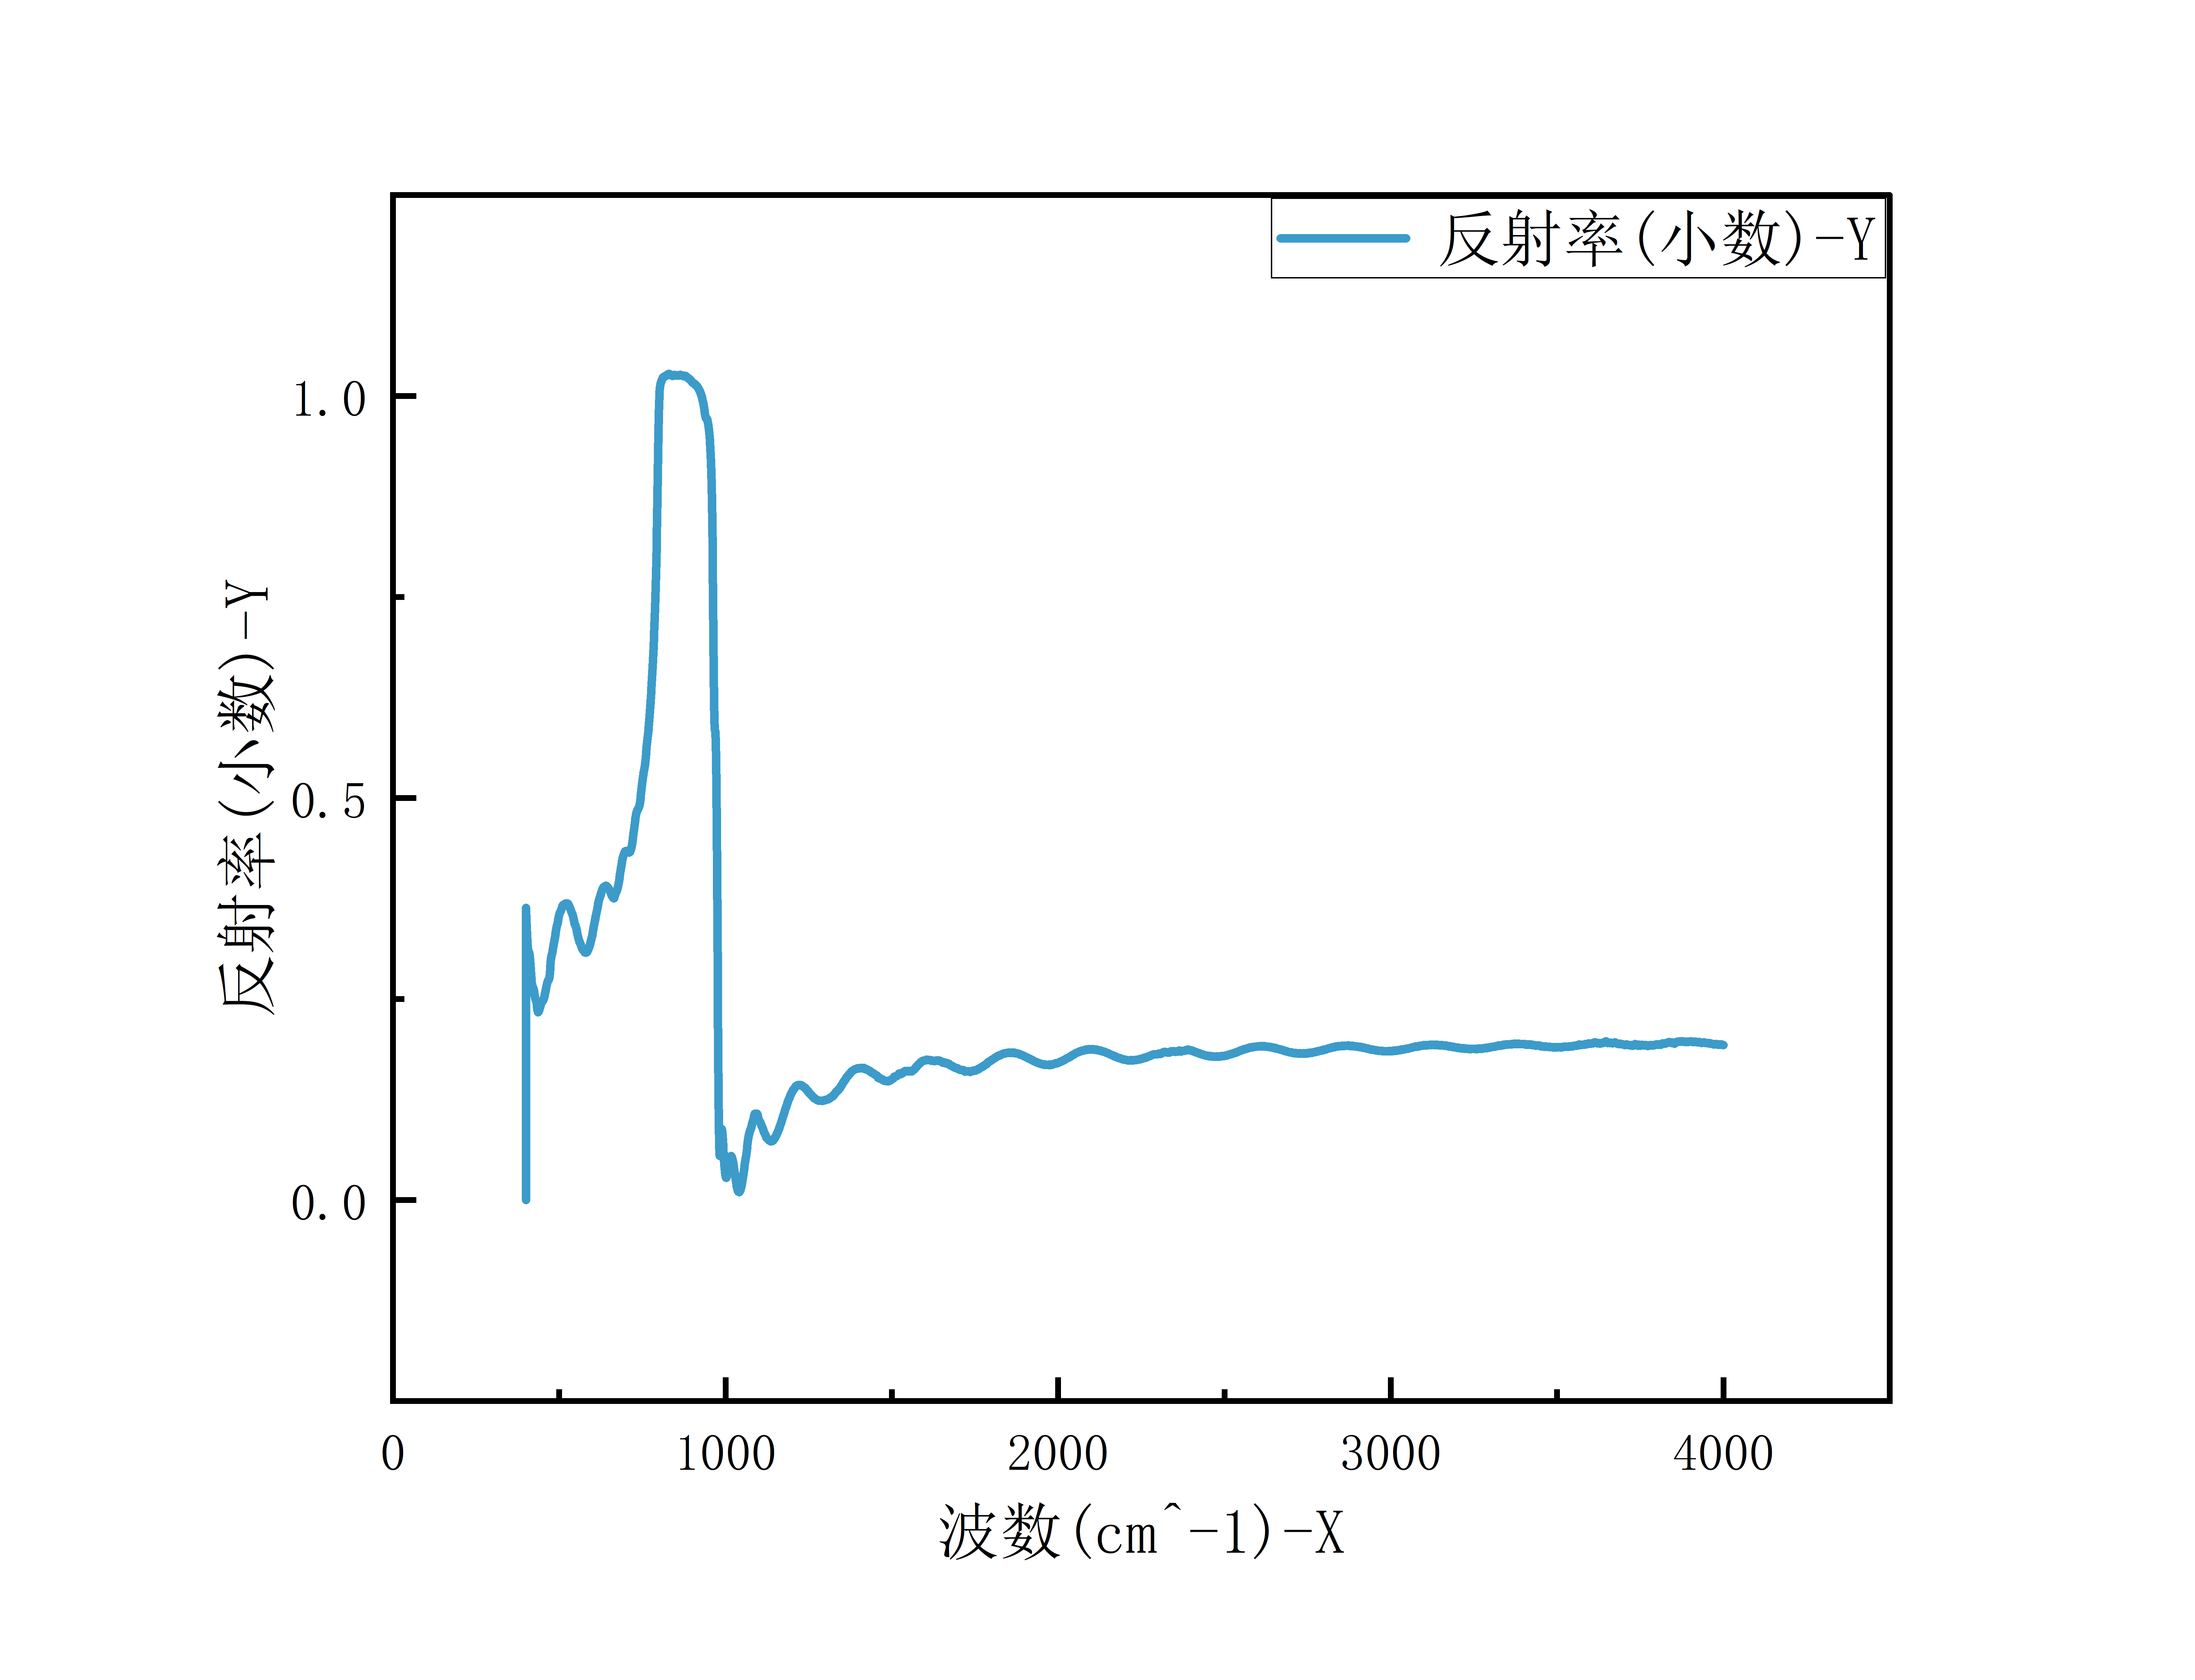
\includegraphics[width=\textwidth]{01_10度原始光谱.png}
			\caption{$10^\circ$ 入射角}
			\label{fig:spec_10}
		\end{subfigure}
		\hfill
		\begin{subfigure}[b]{0.47\textwidth}
			\centering
			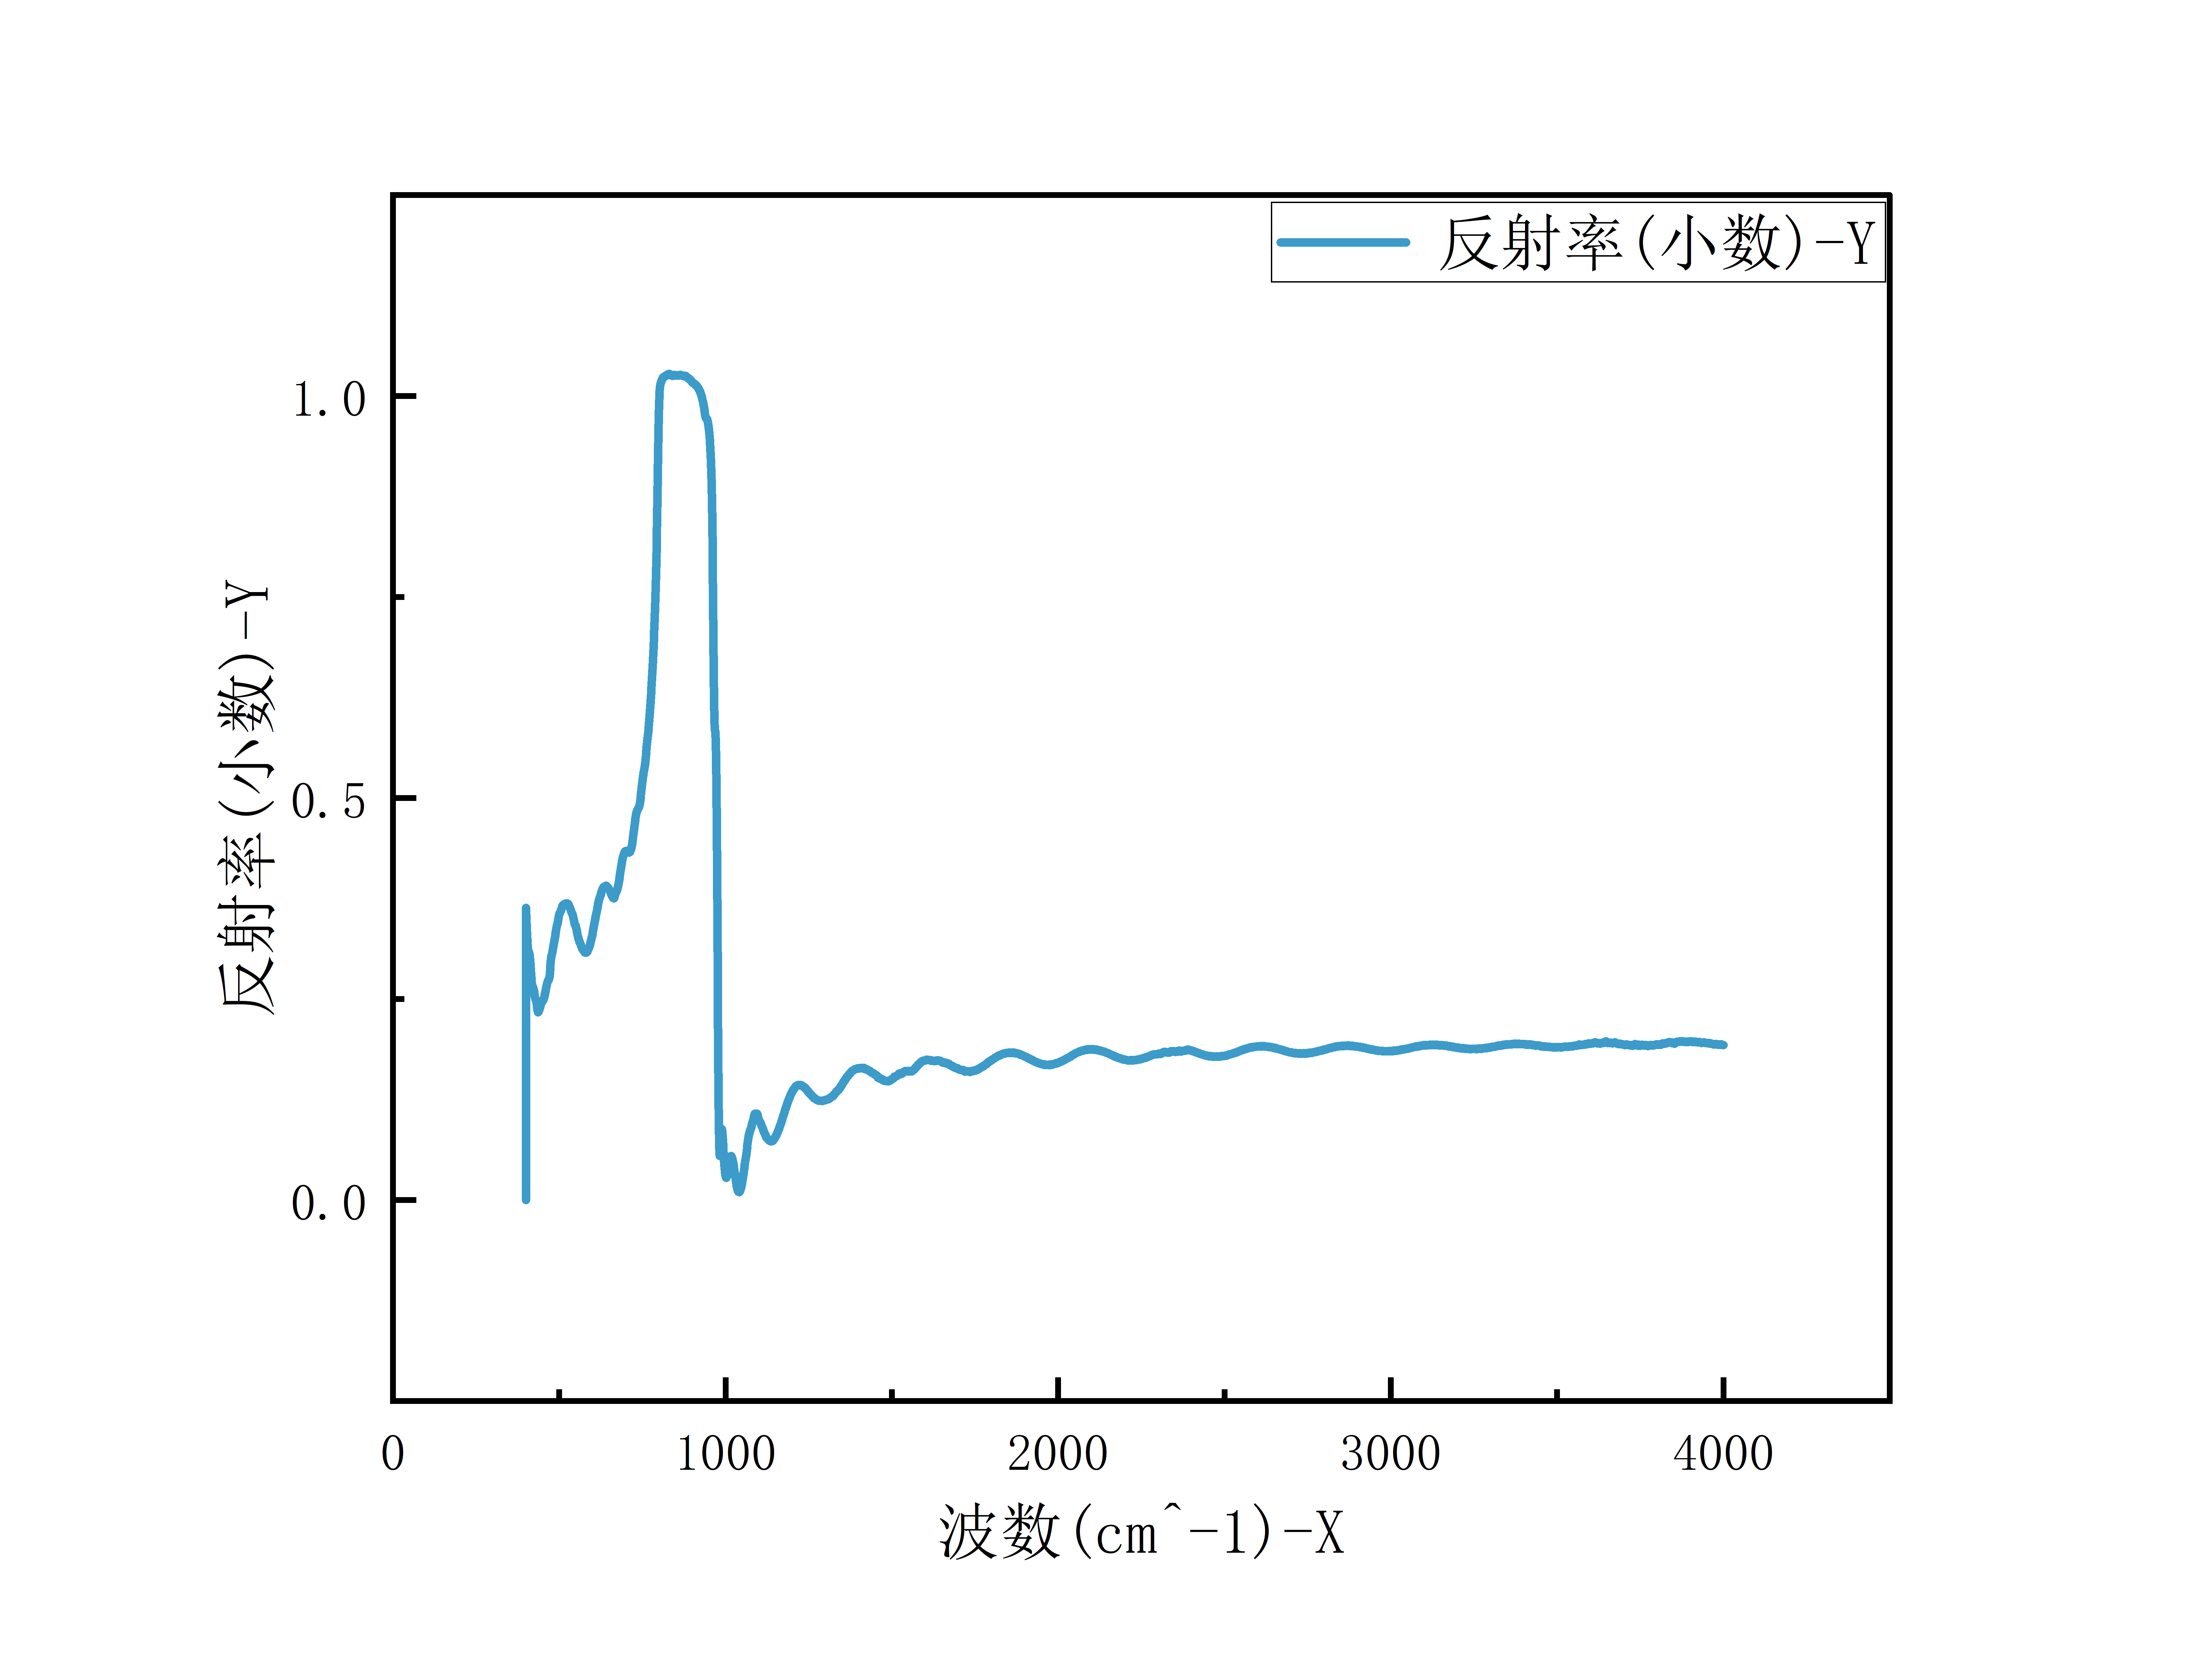
\includegraphics[width=\textwidth]{02_15度原始光谱.png}
			\caption{$15^\circ$ 入射角}
			\label{fig:spec_15}
		\end{subfigure}
		\caption{SiC外延层在两个入射角下的原始反射率光谱对比}
		\label{fig:spec_compare}
	\end{figure}
	
	\subsection{PAPER\_A单角度有界反演模型}
	
	对入射角 $\theta_k\in\{10^\circ,15^\circ\}$，记第 $k$ 个角度的参数为 $\mathbf{p}_k$。问题一建立的非偏振反射率正演算子写作 $R_{\mathrm{th}}(\sigma_i,\theta_k;\mathbf{p}_k)$，单角度最小二乘目标为
	\begin{equation}
		\min_{\mathbf{p}_k} J_k(\mathbf{p}_k) = \sum_{i:2500\le\sigma_i\le3300} [R_{ki} - R_{\mathrm{th}}(\sigma_i,\theta_k;\mathbf{p}_k)]^2.
	\end{equation}
	目标函数关于厚度具有多峰性，因此先固定Sellmeier参数，在厚度、载流子浓度和衬底折射率的网格初值上进行有界最小二乘；再选择不重复的前8个吸引域，释放Sellmeier参数精修。两个角度完全独立运行。最终厚度定义为
	\begin{equation}
		\overline{d} = \frac{d_{10^\circ} + d_{15^\circ}}{2}.
	\end{equation}
	
	图\ref{fig:q2_flow}展示了上述分角度反演的完整流程，清晰呈现了从数据输入到双通道独立优化再到厚度平均的全过程。
	
	\begin{figure}[htbp]
		\centering
		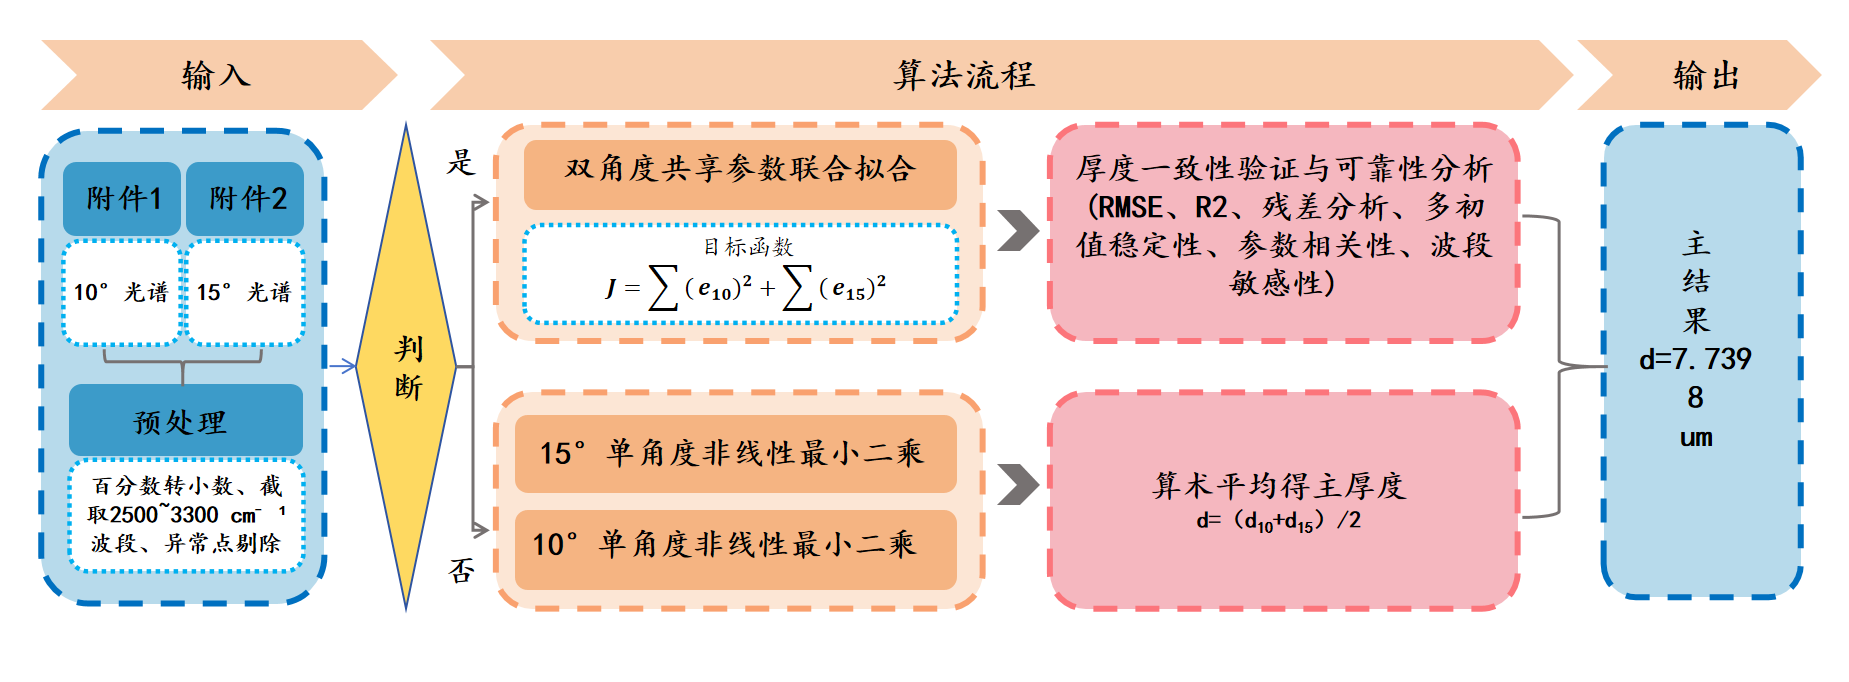
\includegraphics[width=1.0\textwidth]{2.png}
		\caption{问题二分角度有界反演的完整流程图}
		\label{fig:q2_flow}
	\end{figure}
	
	\subsection{求解结果}
	
	两个角度的拟合结果分别为
	\begin{equation}
		d_{10^\circ} = 7.8566\ \mu\mathrm{m},\qquad d_{15^\circ} = 7.6230\ \mu\mathrm{m},
	\end{equation}
	故SiC外延层厚度为
	\begin{equation}
		\boxed{d_{\mathrm{SiC}} = 7.7398\ \mu\mathrm{m}.}
	\end{equation}
	
	两角度结果相差 $0.2337\ \mu\mathrm{m}$，以半极差 $0.1168\ \mu\mathrm{m}$ 表征角度间离散程度。$10^\circ$ 和 $15^\circ$ 拟合的RMSE分别为 $5.9820\times10^{-4}$ 和 $7.0652\times10^{-4}$，$R^2$ 分别为 $0.9551$ 和 $0.9526$。
	
	图\ref{fig:fit_compare}分别展示了 $10^\circ$ 和 $15^\circ$ 入射角下实测光谱与模型拟合曲线的对比。可以看出，模型能够准确重现光谱的峰谷位置和整体趋势，拟合残差在零线附近均匀分布，无明显系统性偏差，验证了双光束模型在弱吸收波段的适用性。其中$15^\circ$的残差在峰谷处略大，反映了大角度下反射系数对角度误差更敏感。
	
	\begin{figure}[htbp]
		\centering
		\begin{subfigure}[b]{0.47\textwidth}
			\centering
			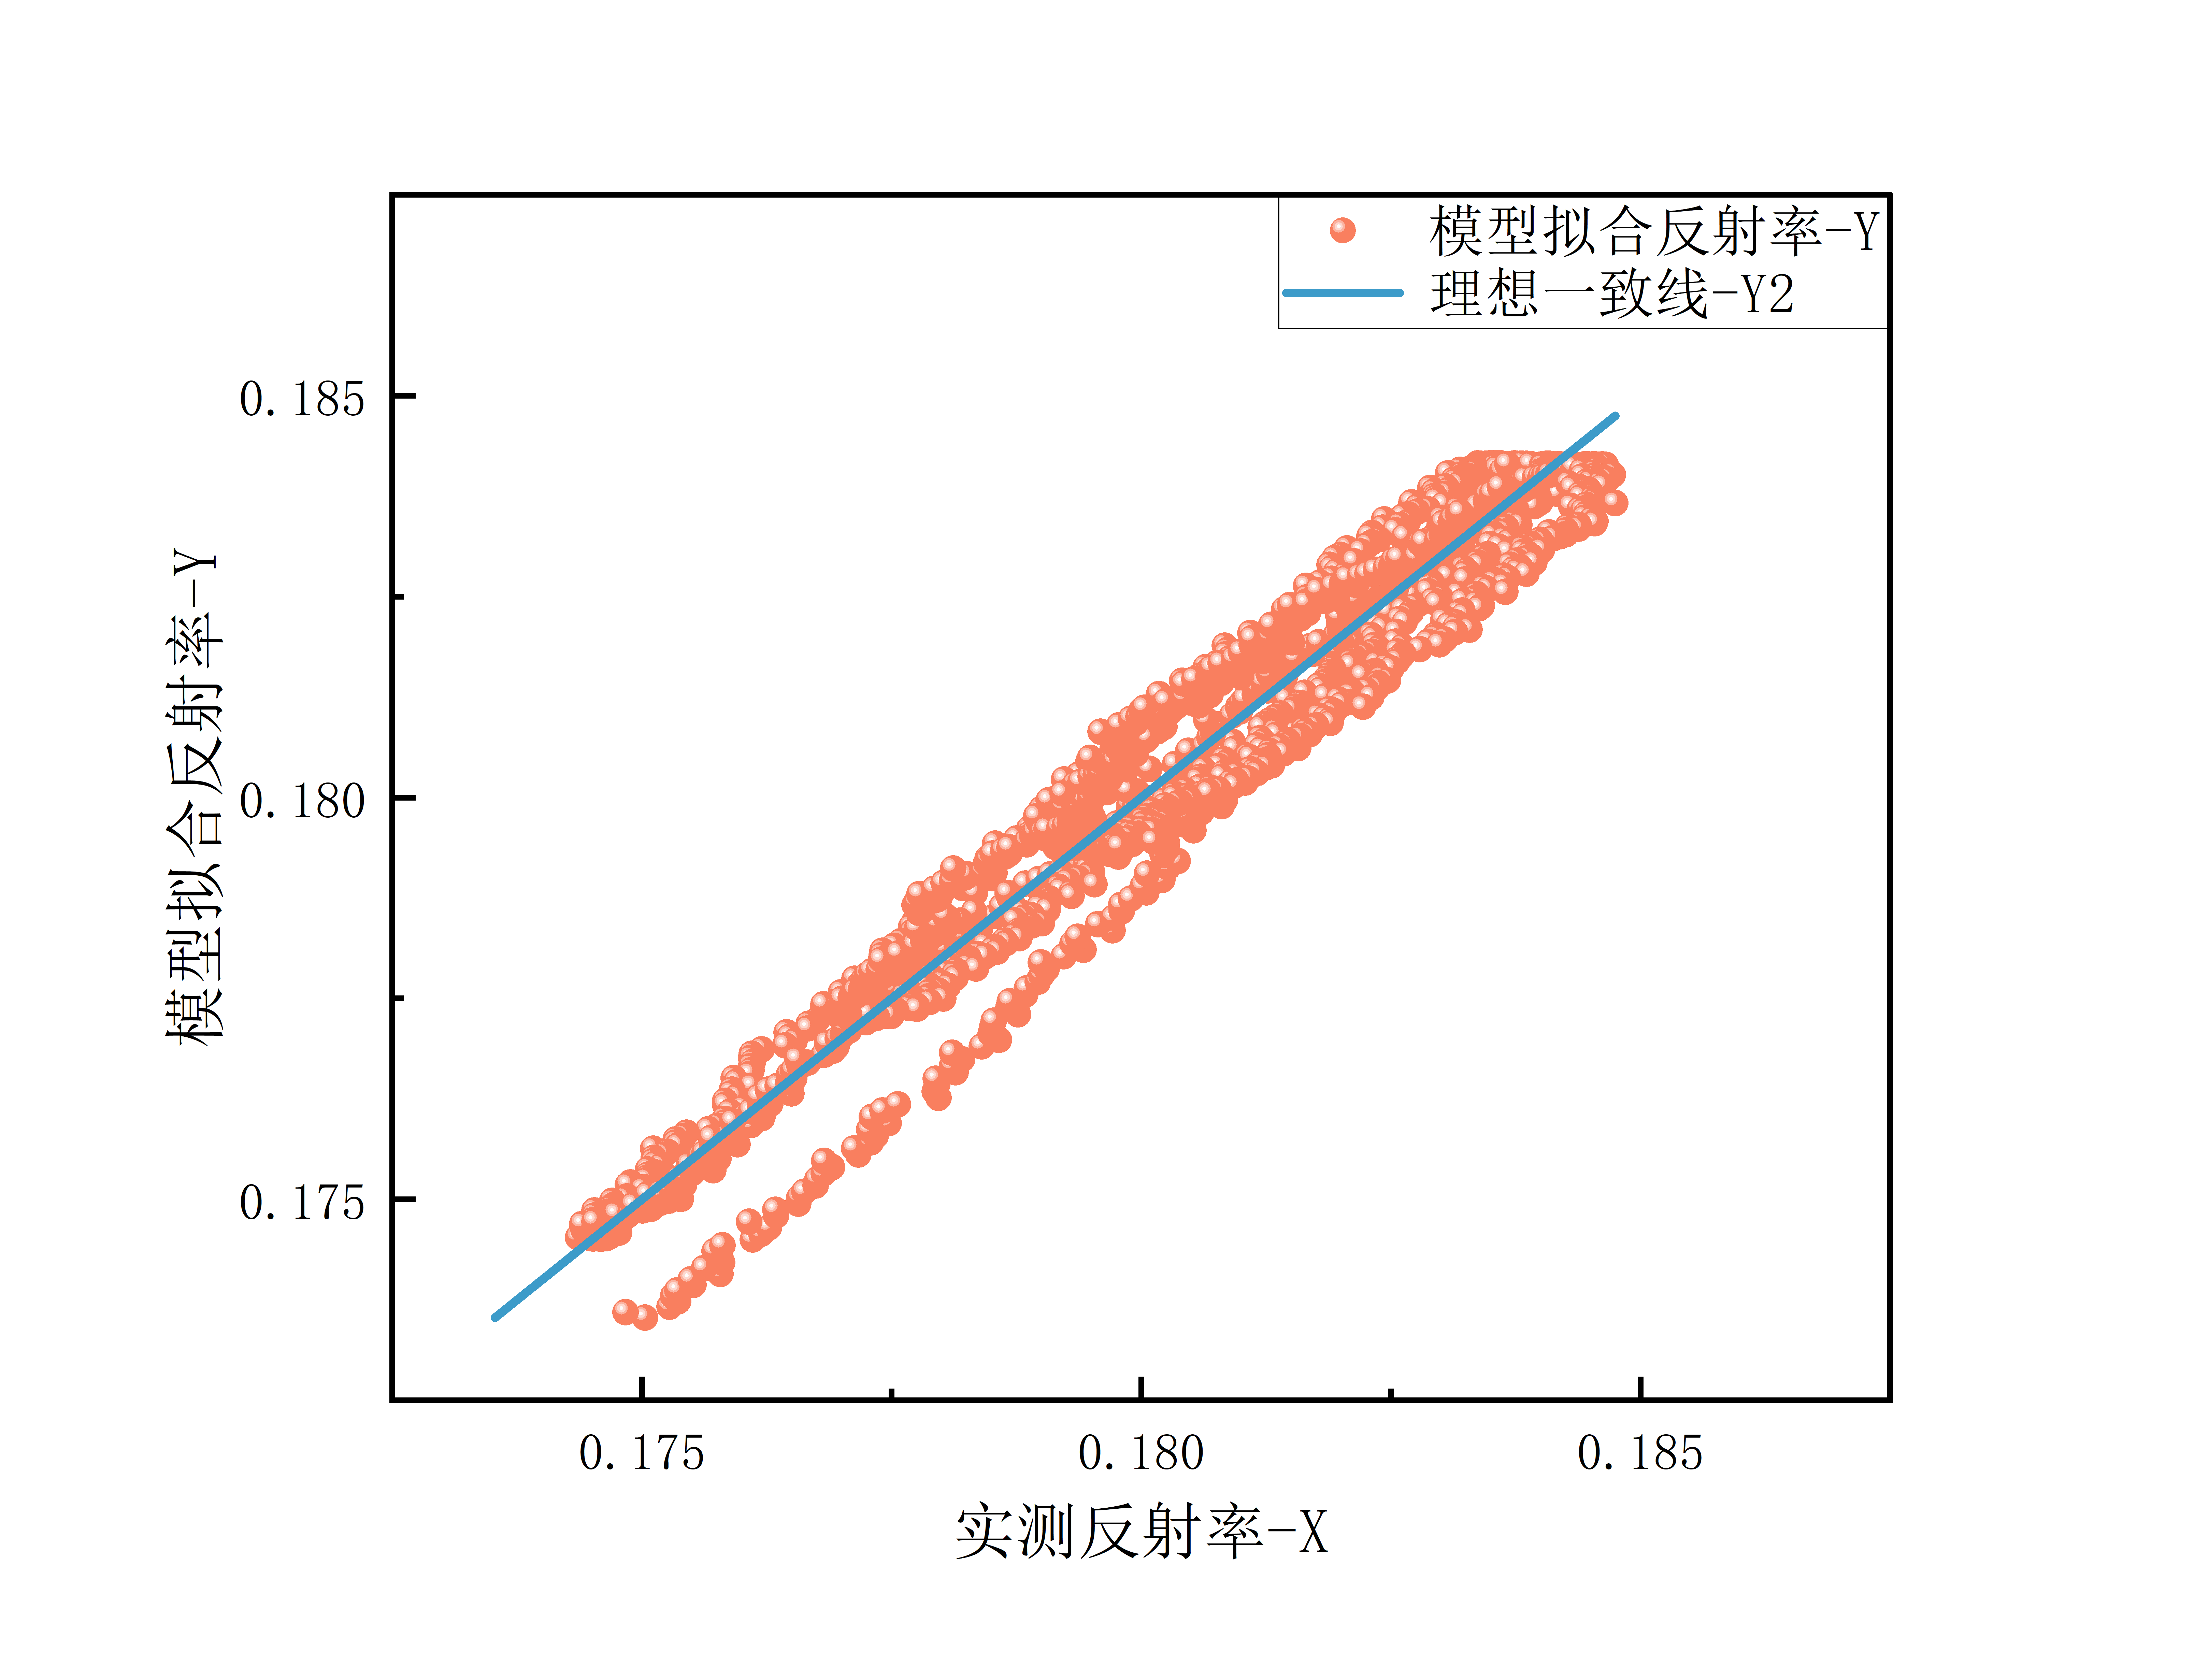
\includegraphics[width=\textwidth]{03_10度实测模型一致性.png}
			\caption{$10^\circ$ 入射角}
			\label{fig:fit_10}
		\end{subfigure}
		\hfill
		\begin{subfigure}[b]{0.47\textwidth}
			\centering
			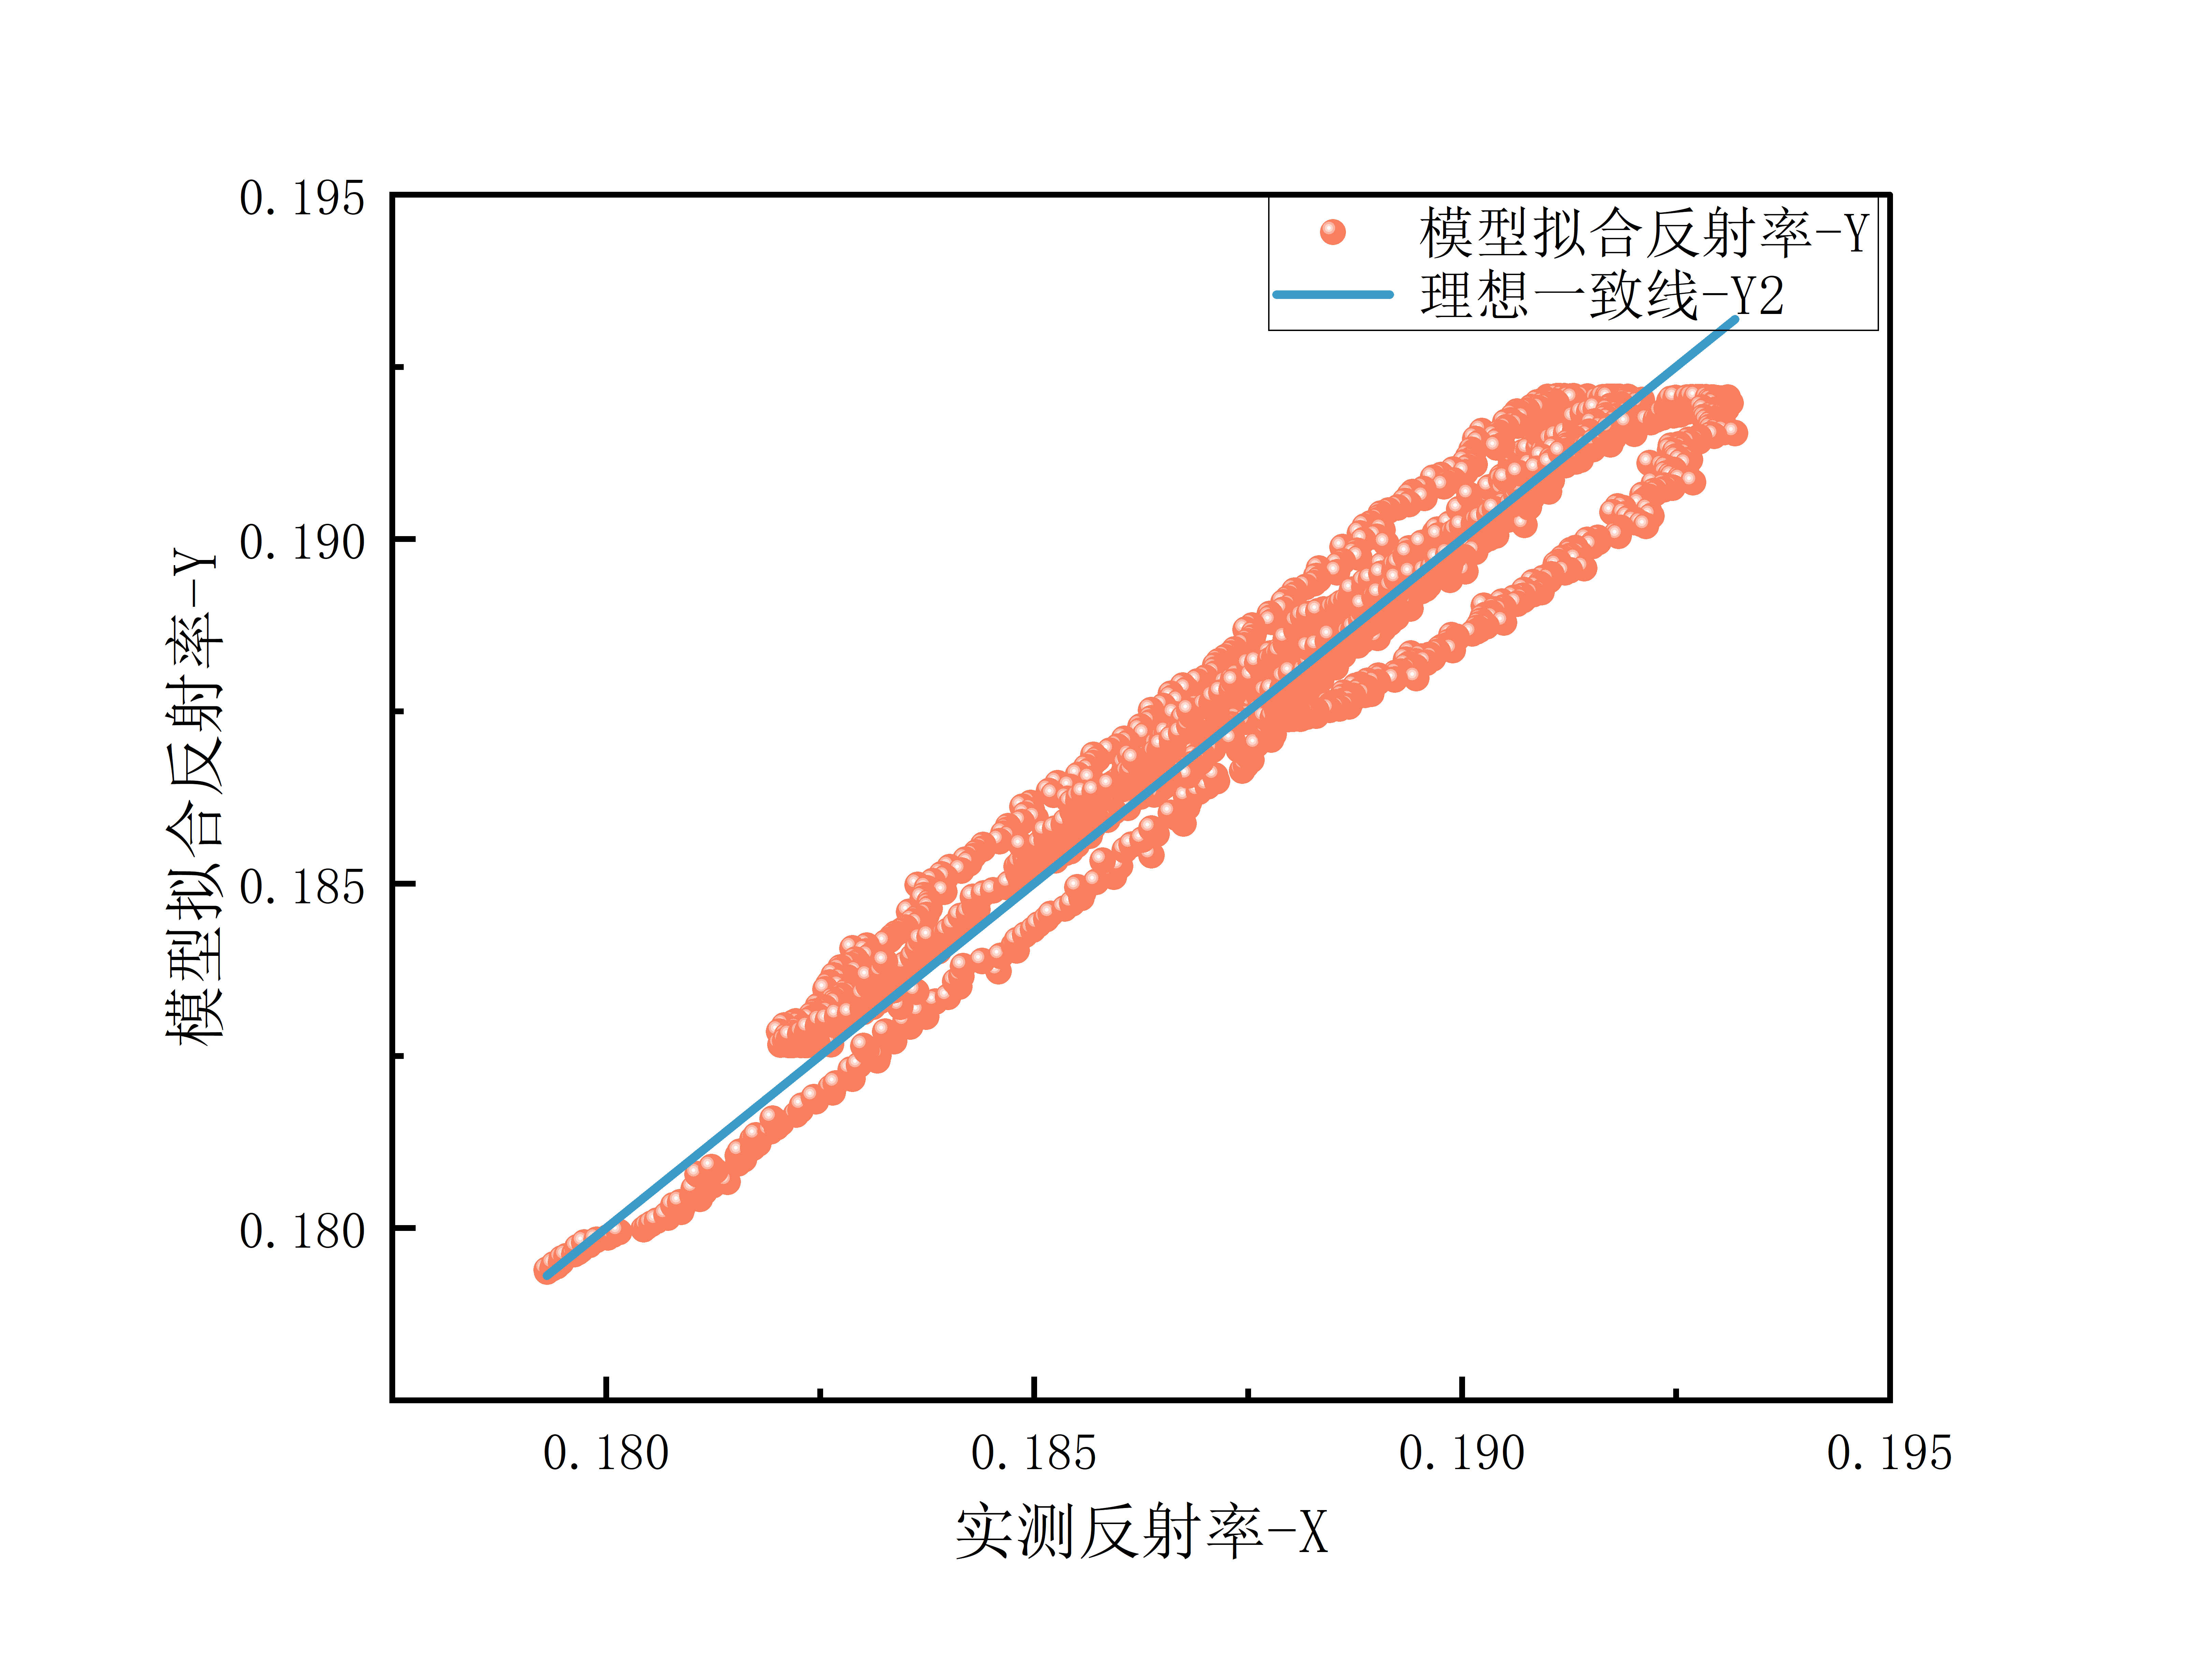
\includegraphics[width=\textwidth]{04_15度实测模型一致性.png}
			\caption{$15^\circ$ 入射角}
			\label{fig:fit_15}
		\end{subfigure}
		\caption{SiC外延层两个入射角下实测光谱与模型拟合对比及残差分布}
		\label{fig:fit_compare}
	\end{figure}
	
	\begin{table}[htbp]
		\centering
		\caption{问题二单角度反演结果}
		\label{tab:q2_results}
		\begin{tabular}{cccc}
			\toprule
			\rowcolor{cyan!20}\bfseries
			\textbf{入射角} & \textbf{厚度/$\mu\mathrm{m}$} & \textbf{RMSE} & \textbf{$R^2$} \\
			\midrule
			$10^\circ$ & 7.8566 & $5.9820\times10^{-4}$ & 0.9551 \\
			$15^\circ$ & 7.6230 & $7.0652\times10^{-4}$ & 0.9526 \\
			\rowcolor{gray!8}
			平均 & \textbf{7.7398} & — & — \\
			\bottomrule
		\end{tabular}
	\end{table}
	
	\subsection{结果可靠性分析}
	
	为全面评估反演结果的可靠性和模型拟合质量，从残差分布、拟合优度指标、多初值收敛性和残差正态性等方面进行系统检验。
	
	\subsubsection{残差分布分析}
	
	图\ref{fig:resid_scatter}展示了所有数据点绝对残差的散点分布。残差主要集中在 $-0.005$ 至 $0.005$ 范围内，无明显趋势或异方差性，表明模型假设与数据一致。散点在波数轴上分布均匀，说明模型在不同波段表现稳定。
	
	\begin{figure}[htbp]
		\centering
		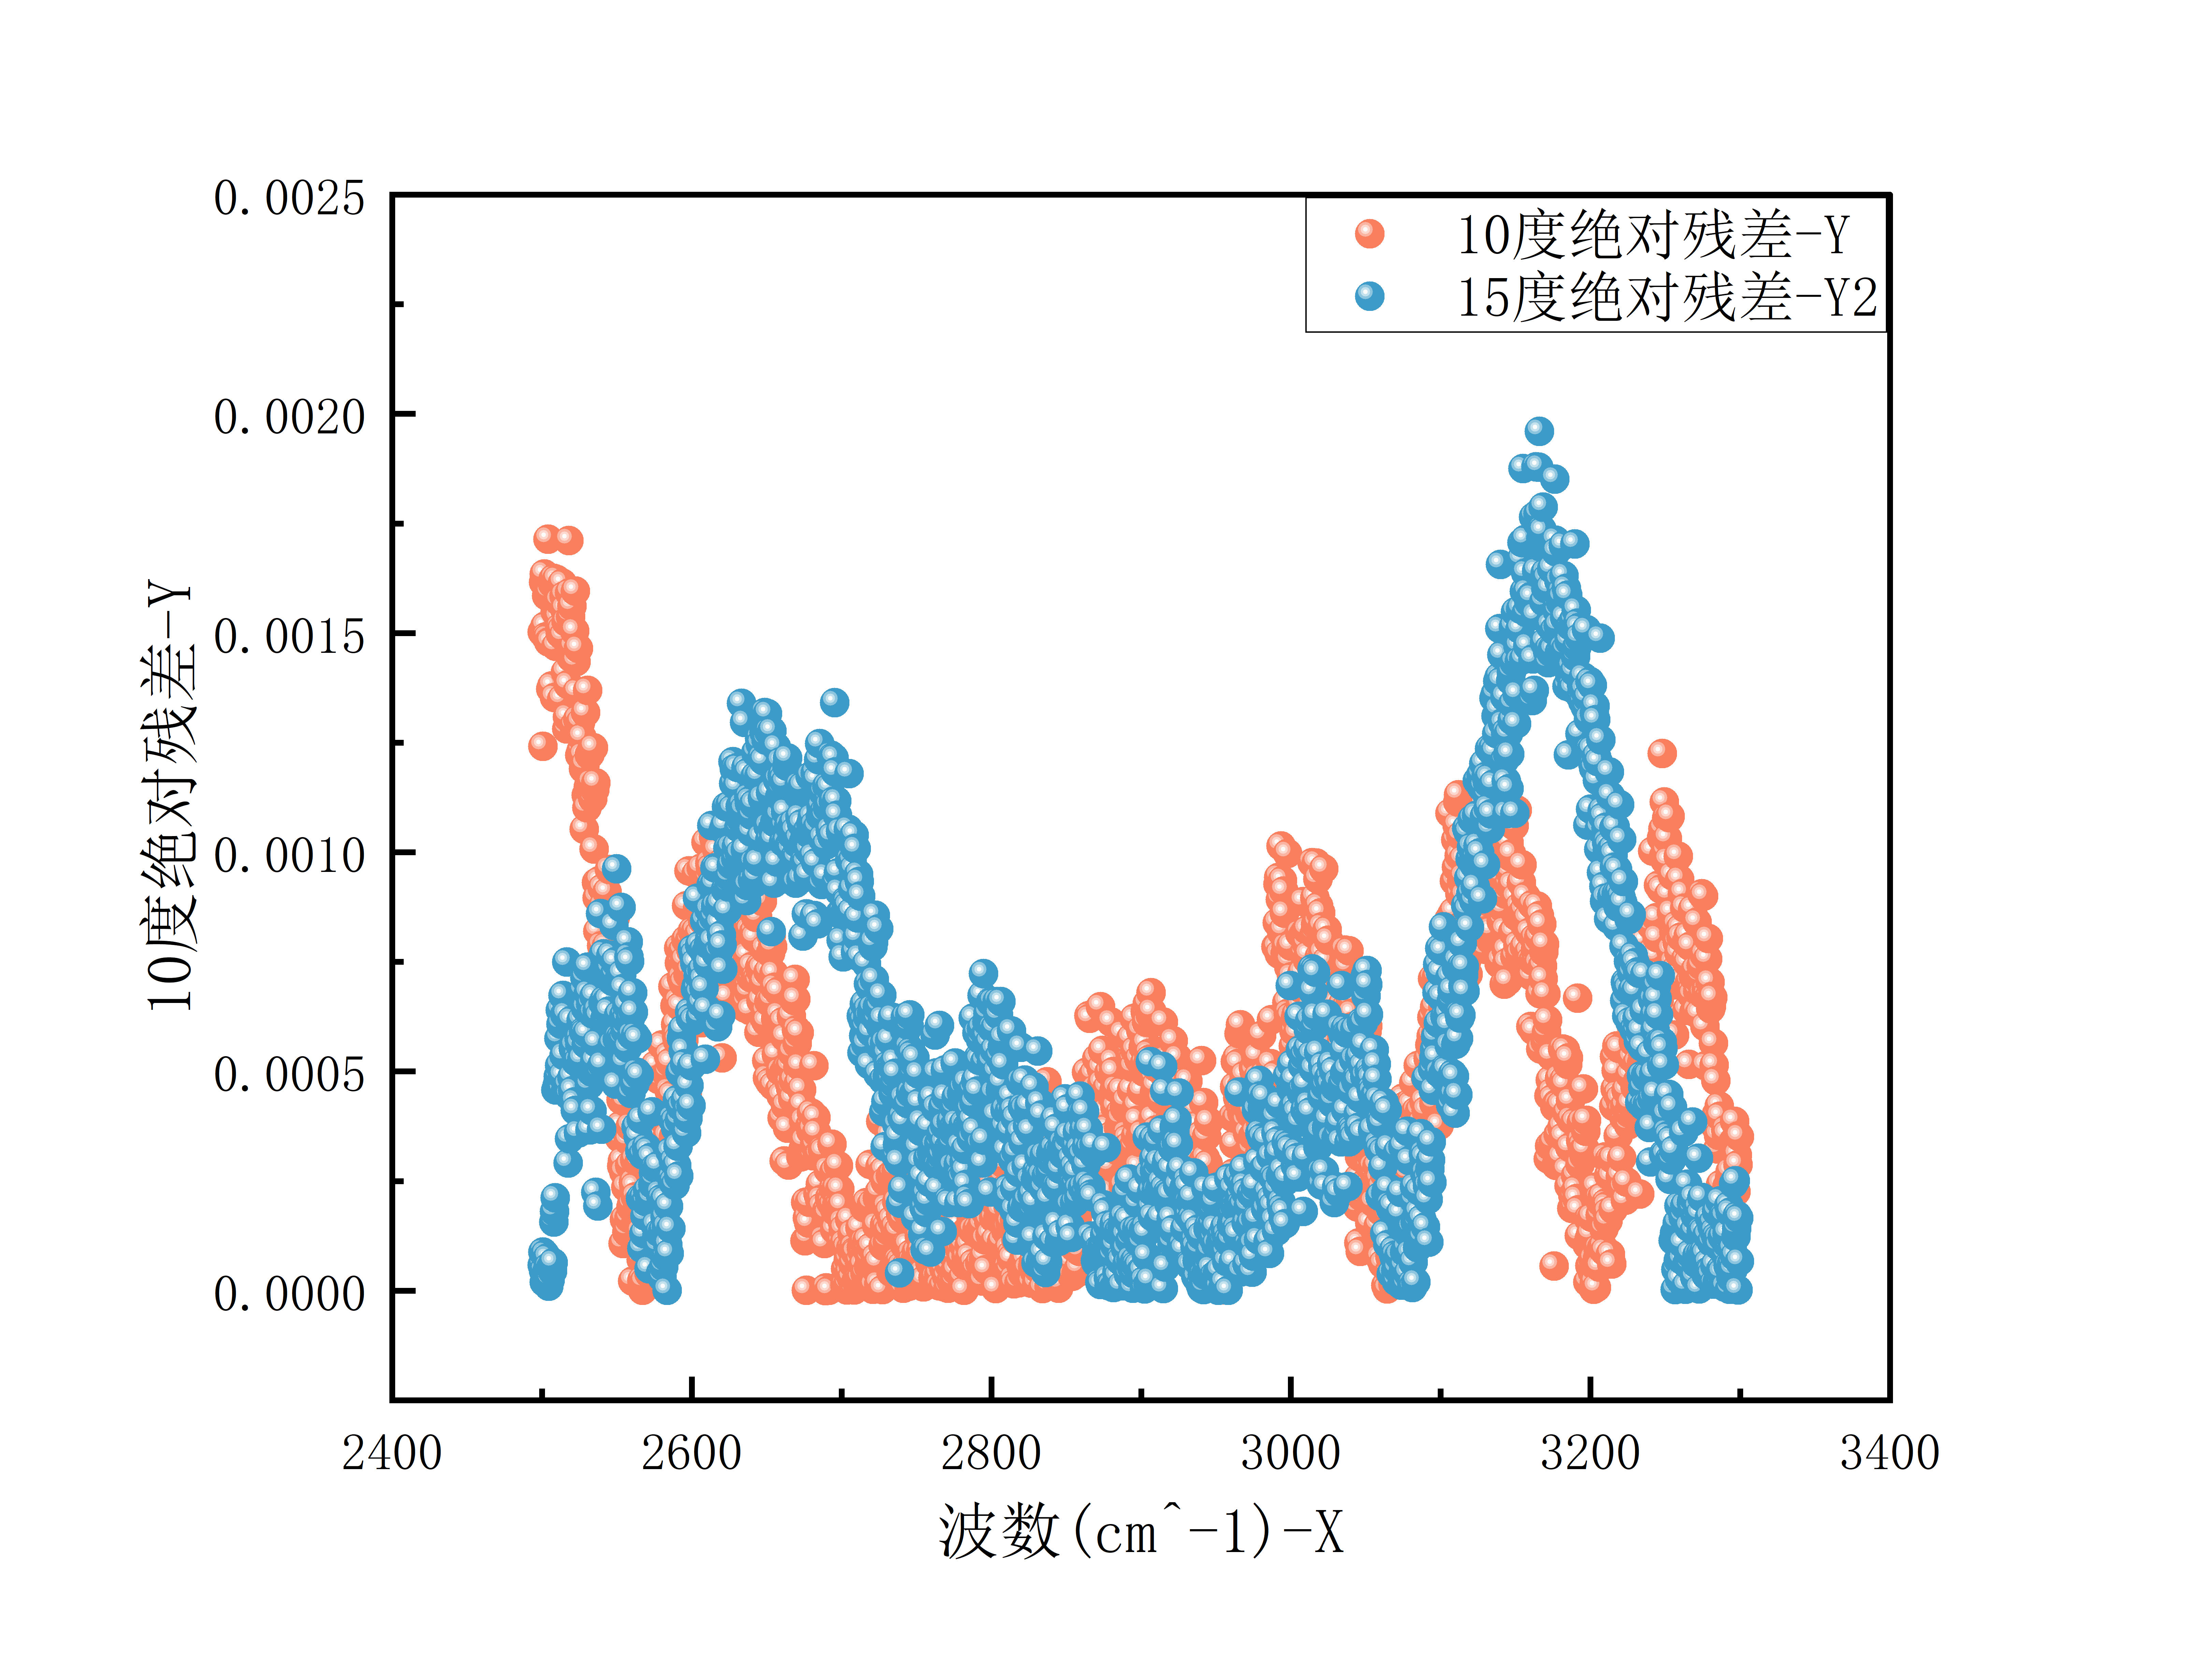
\includegraphics[width=0.7\textwidth]{05_绝对残差散点.png}
		\caption{所有数据点的绝对残差散点图}
		\label{fig:resid_scatter}
	\end{figure}
	
	图\ref{fig:resid_grouped_box}将残差按波数区间分组并对比各组的均值与标准差。各波段残差均值均接近零，标准差量级一致（约$0.003\sim0.005$），进一步确认模型在各波段表现均匀，不存在某个波段系统偏差显著增大的问题。
	
	\begin{figure}[htbp]
		\centering
		\begin{subfigure}[b]{0.47\textwidth}
			\centering
			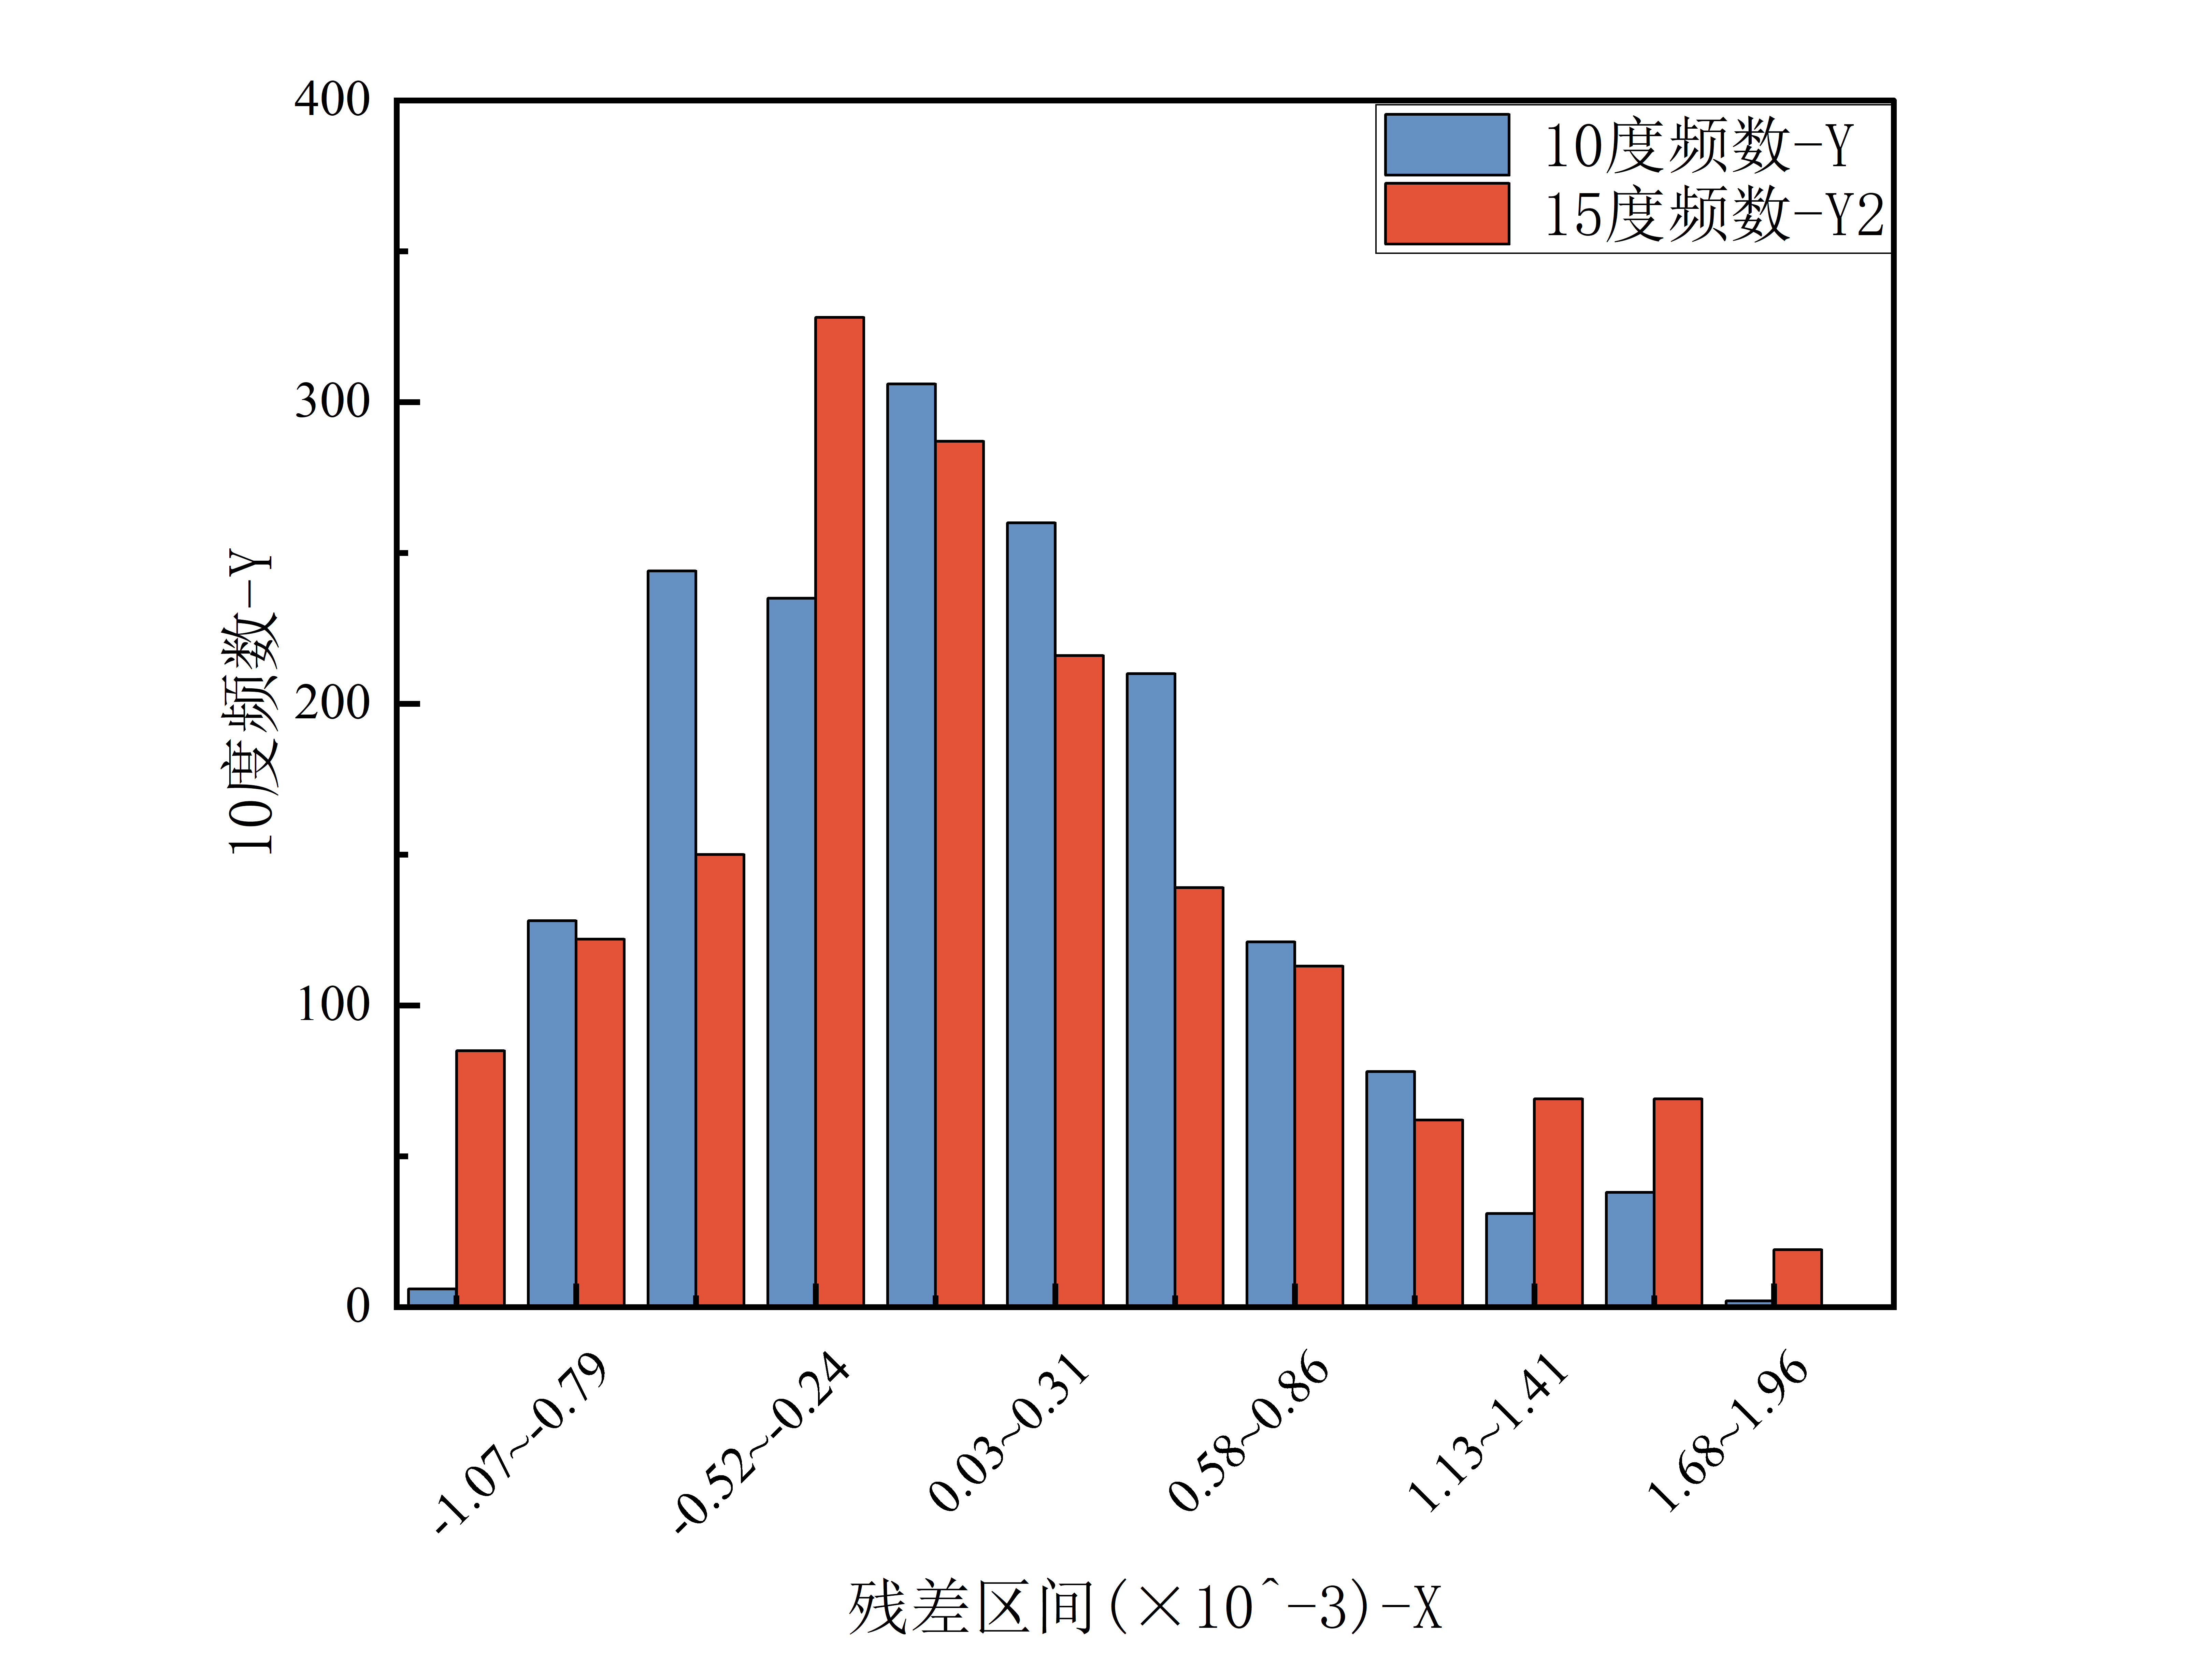
\includegraphics[width=\textwidth]{06_残差分组柱状图.png}
			\caption{分组柱状图（均值$\pm$标准差）}
			\label{fig:resid_grouped}
		\end{subfigure}
		\hfill
		\begin{subfigure}[b]{0.47\textwidth}
			\centering
			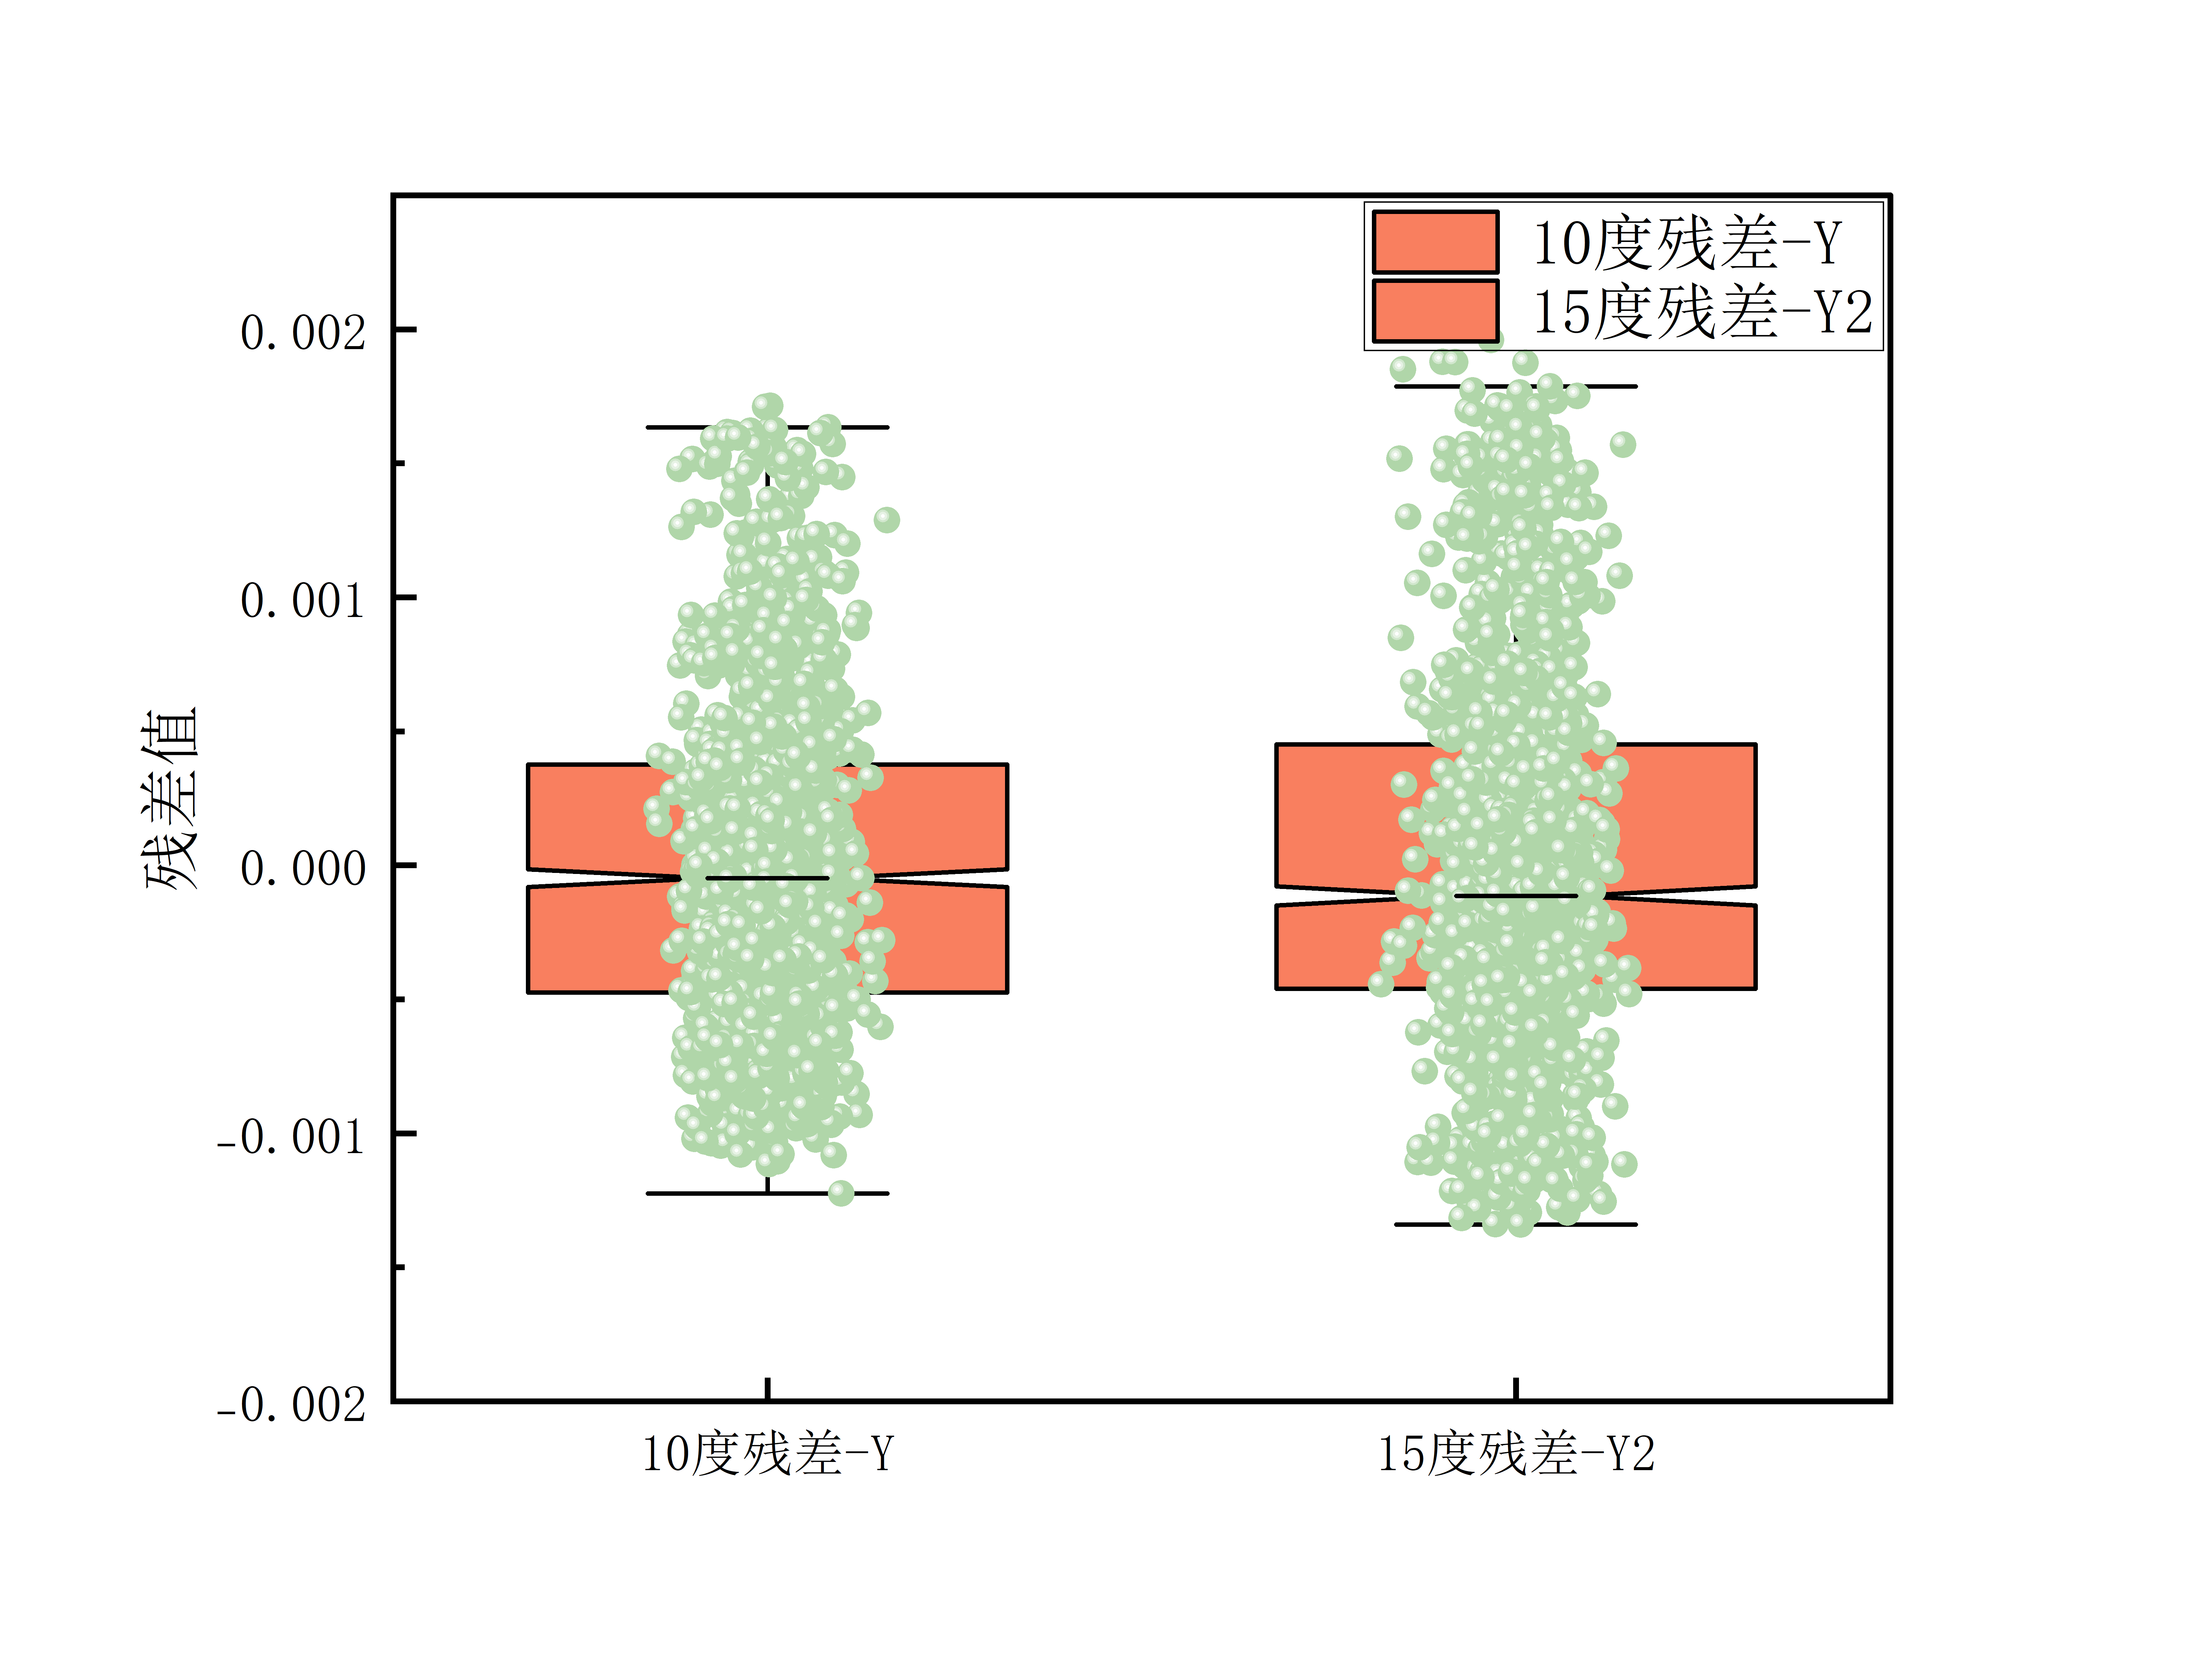
\includegraphics[width=\textwidth]{07_残差箱线图.png}
			\caption{箱线图汇总}
			\label{fig:resid_box}
		\end{subfigure}
		\caption{残差分组统计与箱线图}
		\label{fig:resid_grouped_box}
	\end{figure}
	
	图\ref{fig:resid_heat}以热力图形式展示残差在波数—反射率平面上的密度分布，颜色越深表示该区域数据点越多。热力中心集中在零线附近，表明系统偏差极小；高温区域沿零线呈带状延伸，说明模型在整个波段范围内均保持较高的拟合精度。
	
	\begin{figure}[htbp]
		\centering
		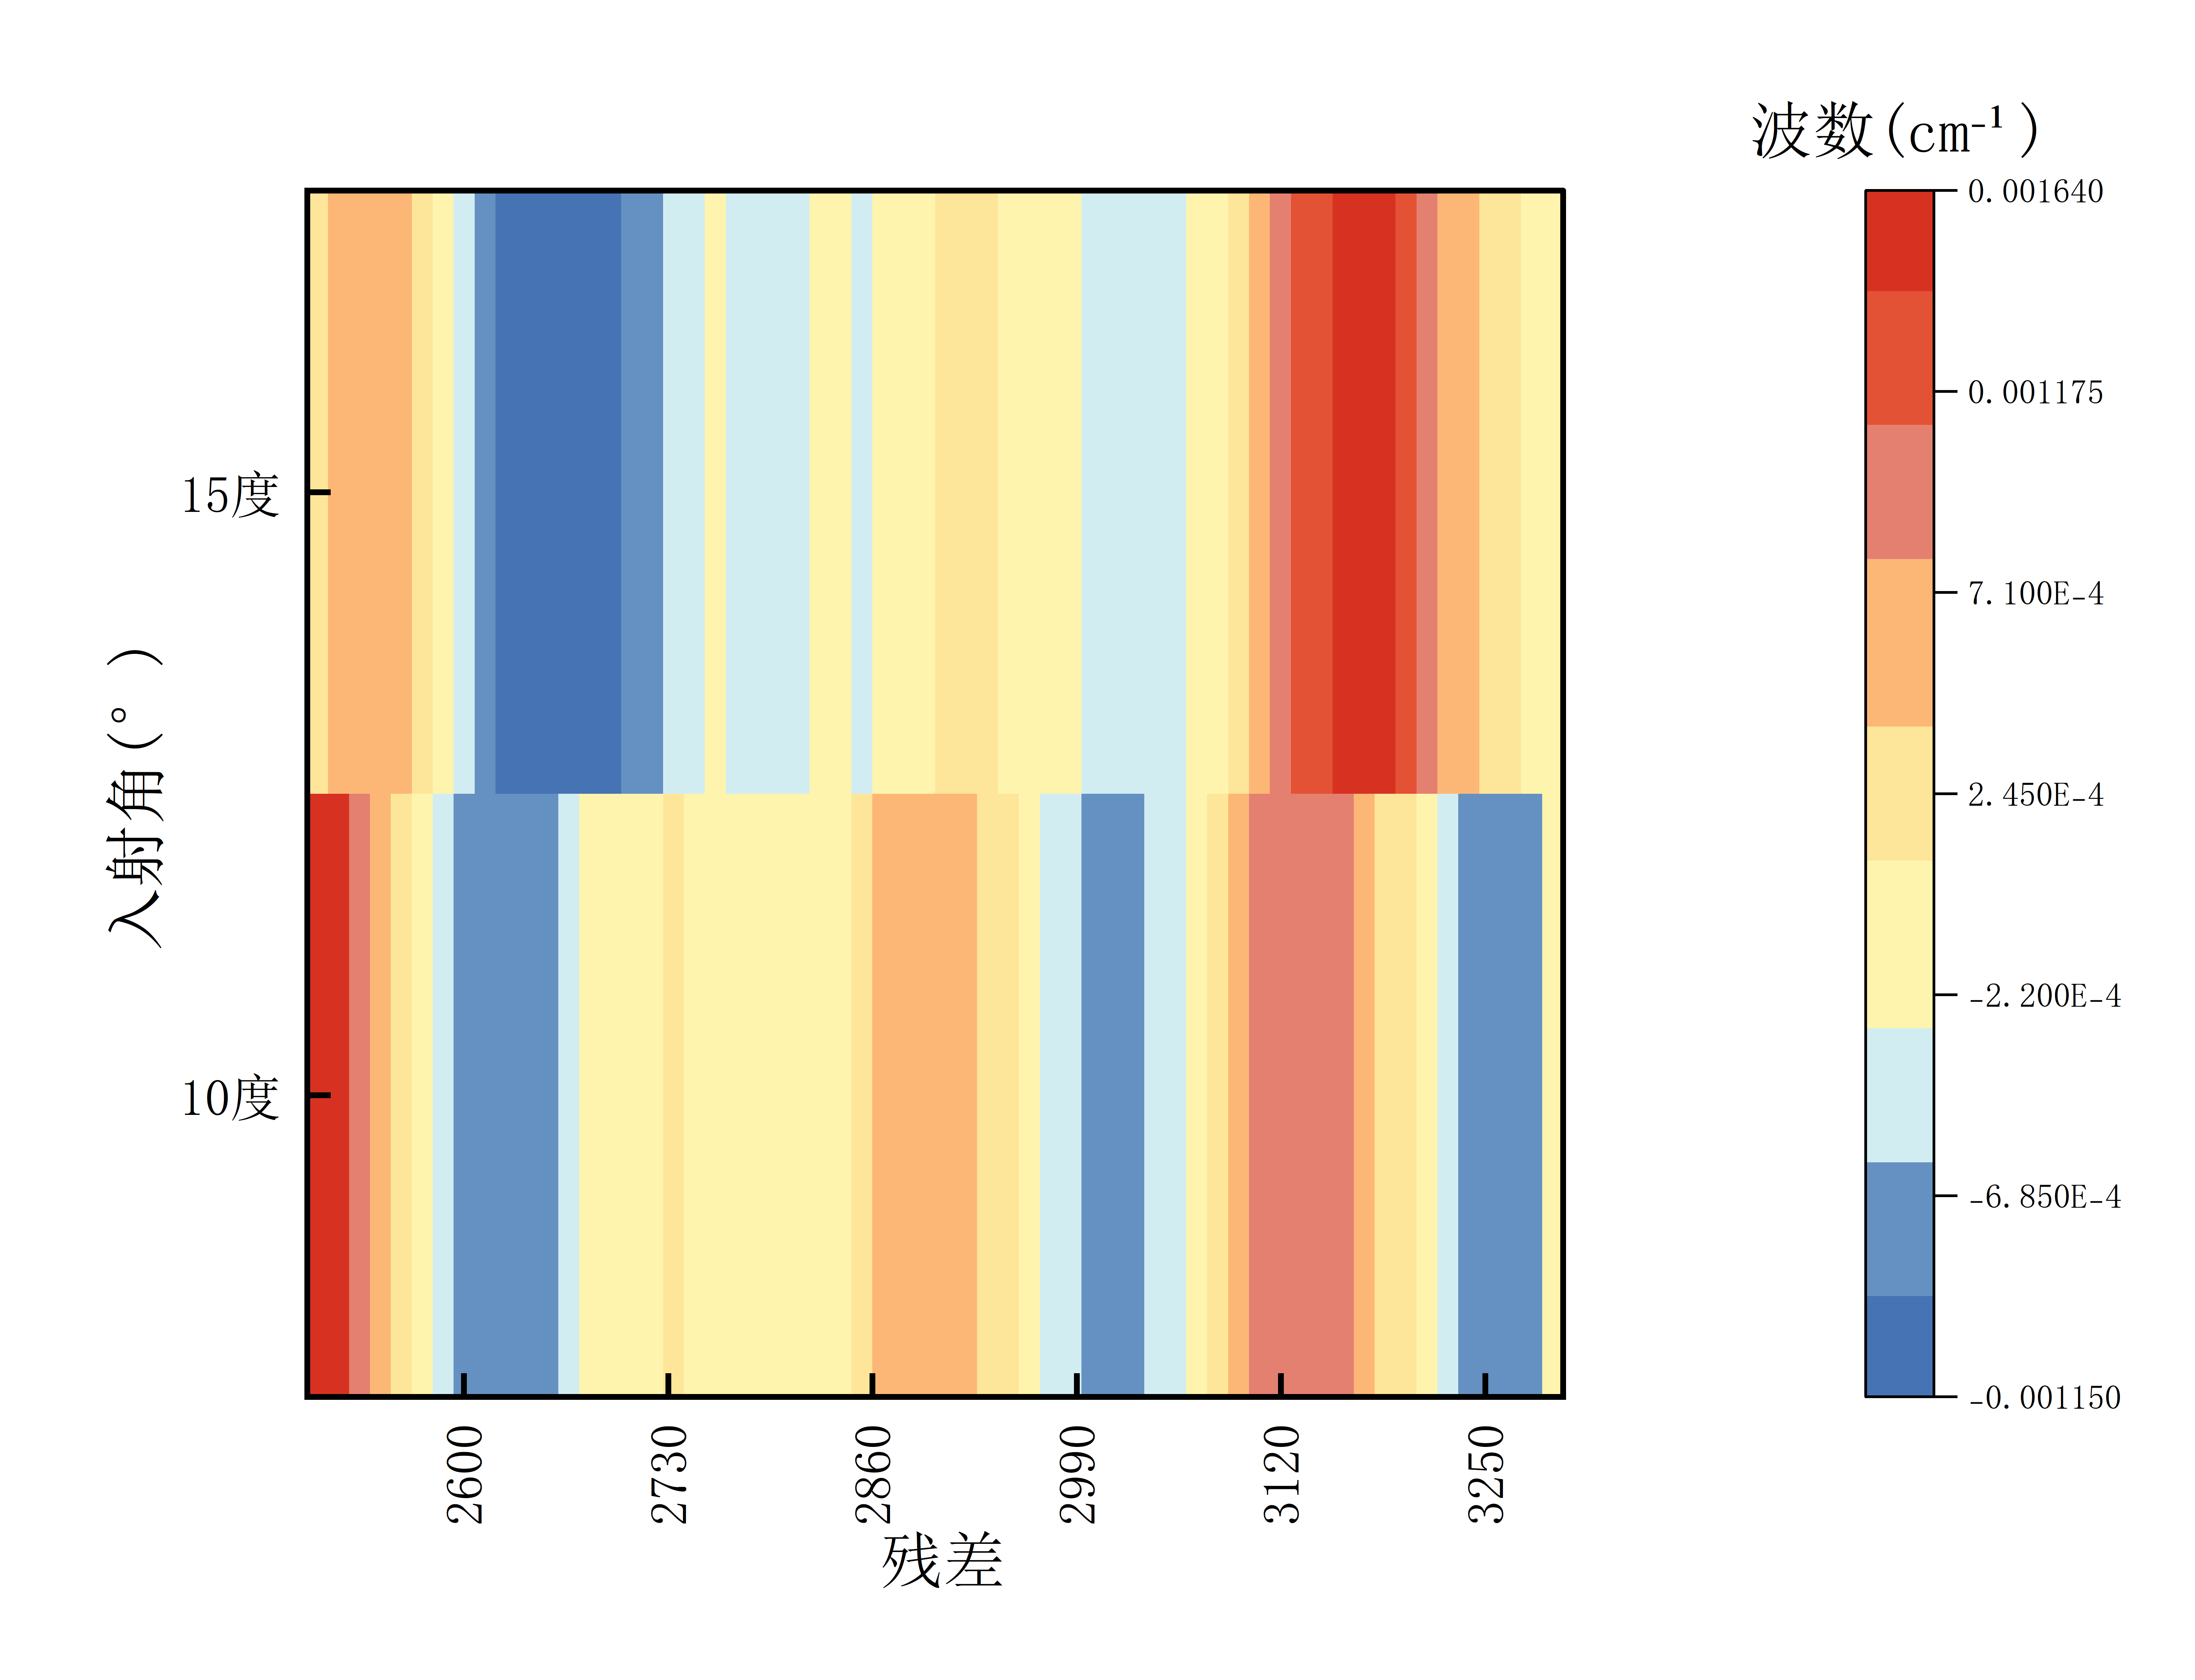
\includegraphics[width=0.7\textwidth]{08_残差热力图.png}
		\caption{残差在波数—反射率平面上的二维密度热力图}
		\label{fig:resid_heat}
	\end{figure}
	
	\subsubsection{拟合优度与厚度稳定性}
	
	图\ref{fig:thickness_metrics}以柱状图对比了厚度反演结果及RMSE和MAPE两个拟合优度指标。厚度柱状图显示两个角度结果高度一致，置信区间重叠；RMSE和MAPE指标显示$10^\circ$的拟合精度略优于$15^\circ$，而后续$R^2$指标（图\ref{fig:r2_bar}）显示两角度均在0.95以上，证实模型在两种角度下均能有效解释光谱变化。
	
	\begin{figure}[htbp]
		\centering
		\begin{subfigure}[b]{0.31\textwidth}
			\centering
			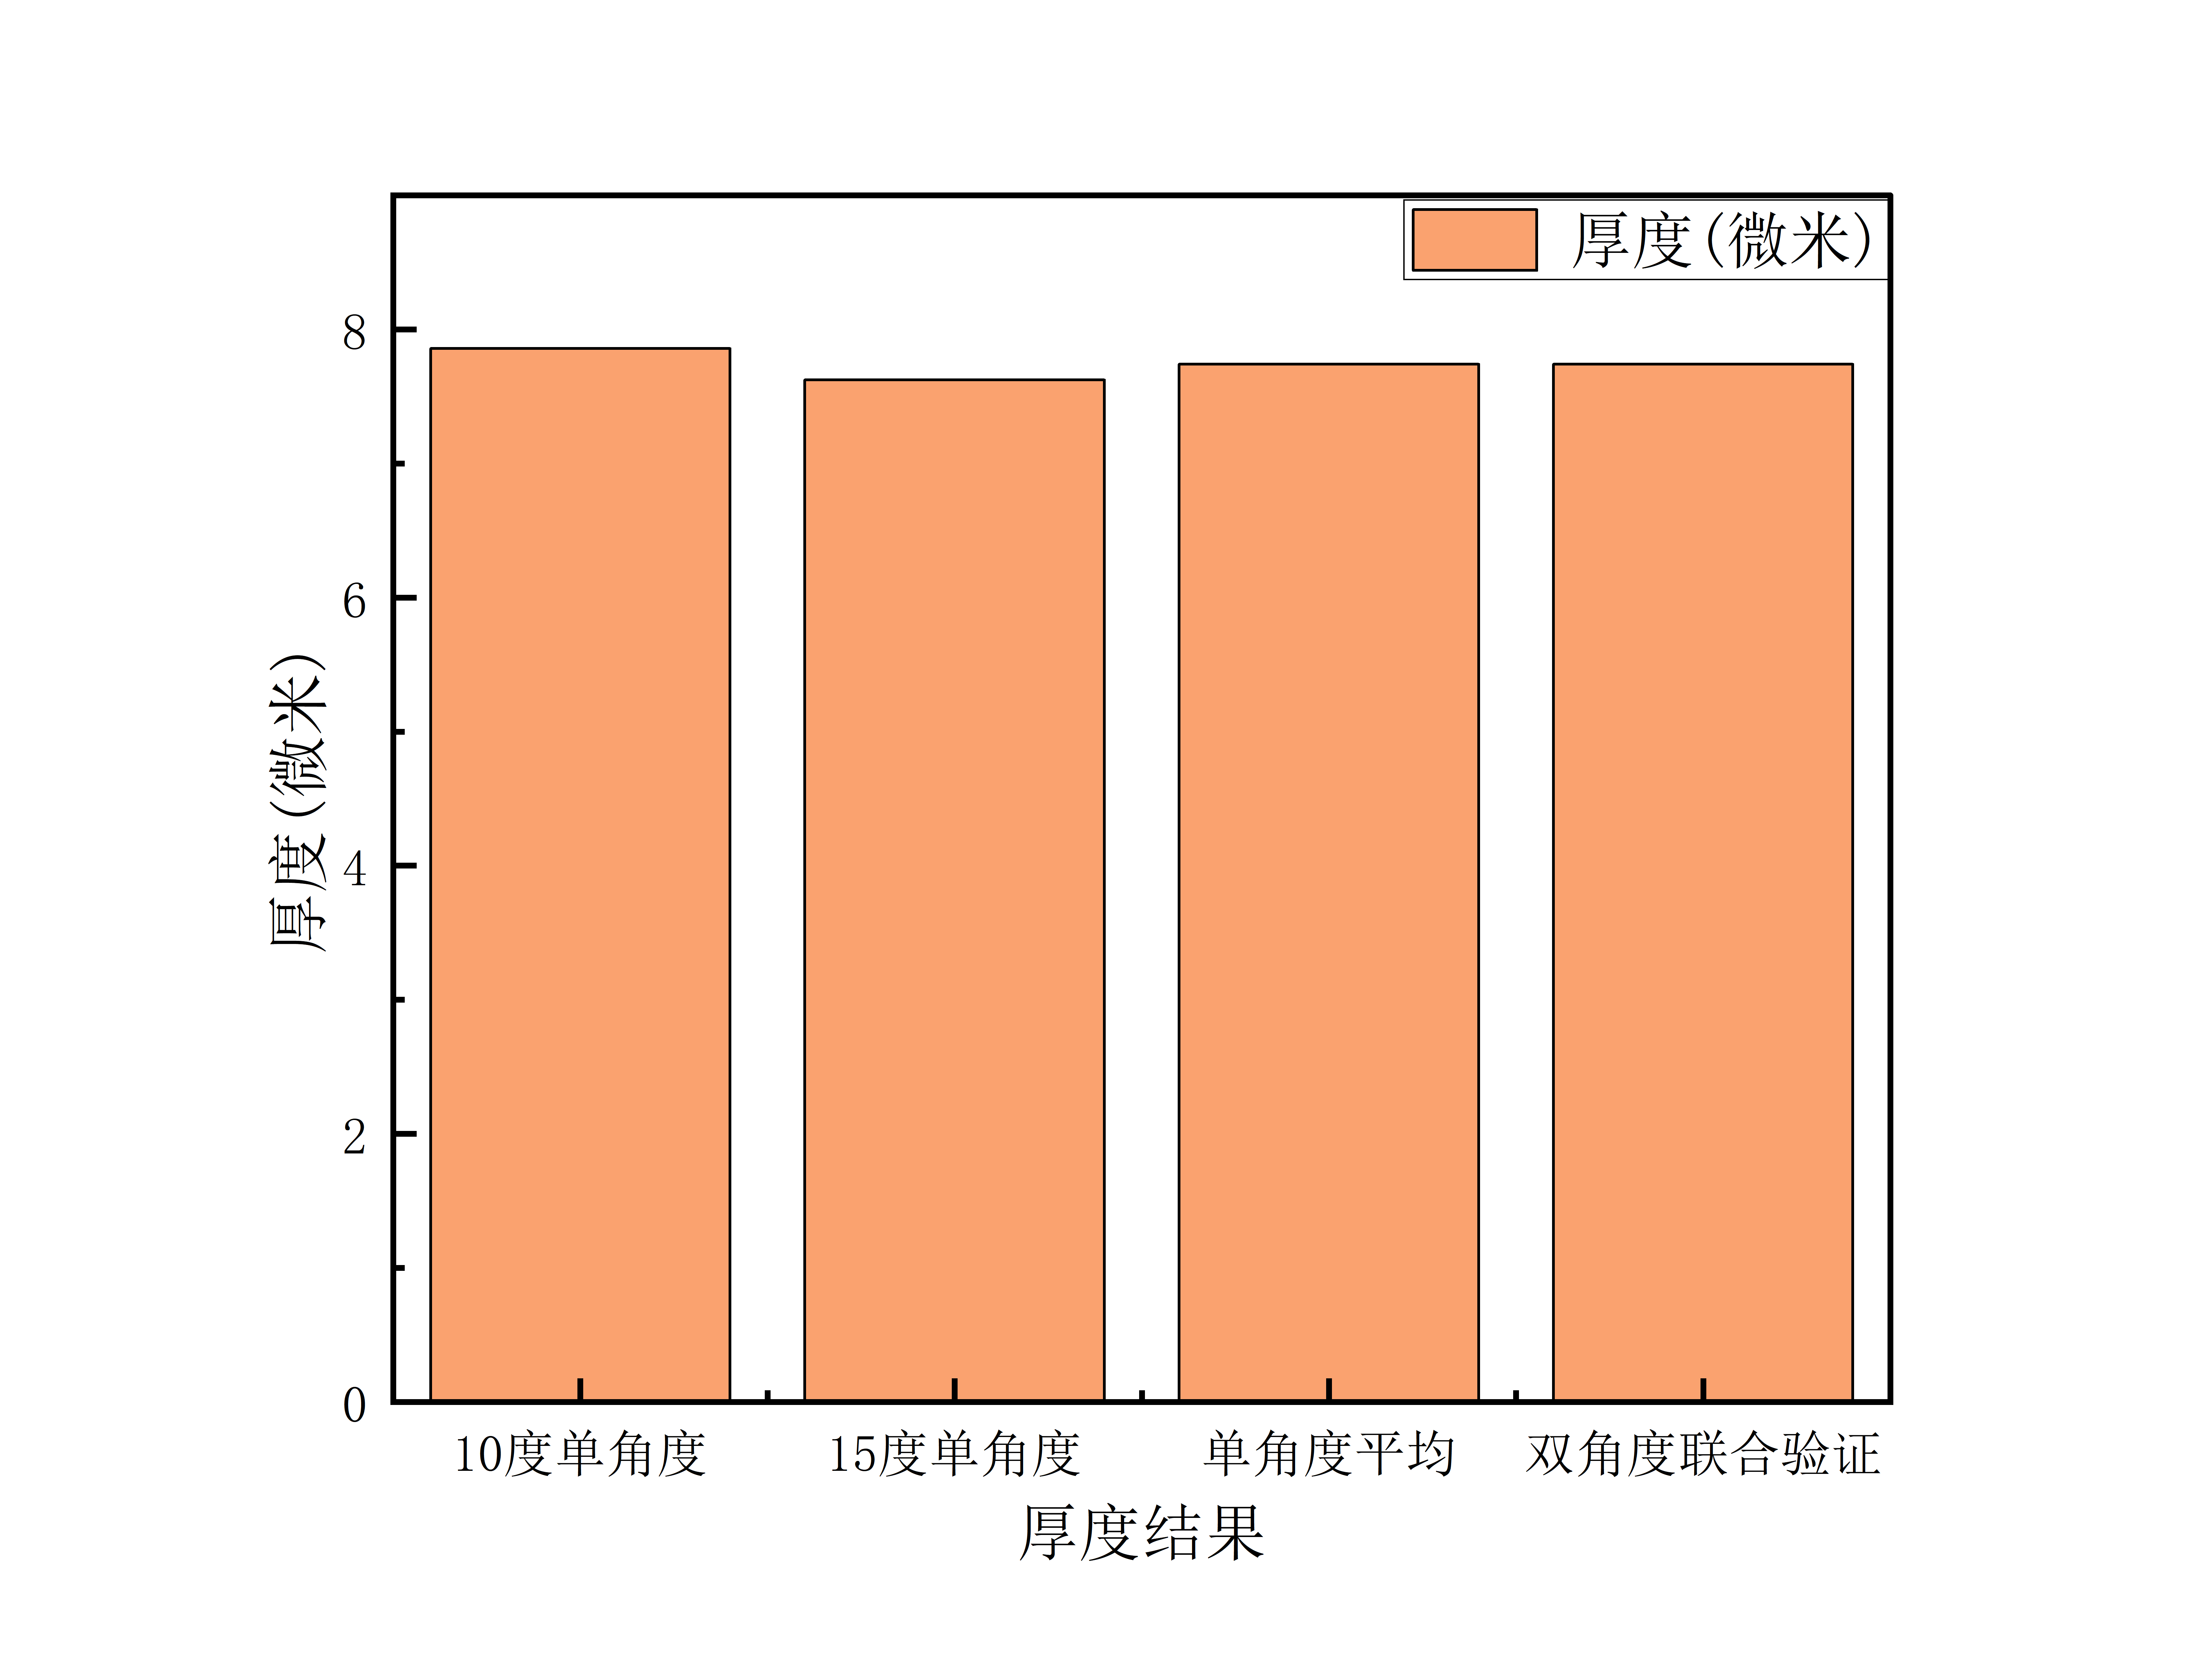
\includegraphics[width=\textwidth]{09_厚度结果柱状图.png}
			\caption{厚度反演结果}
			\label{fig:thickness_bar}
		\end{subfigure}
		\hfill
		\begin{subfigure}[b]{0.31\textwidth}
			\centering
			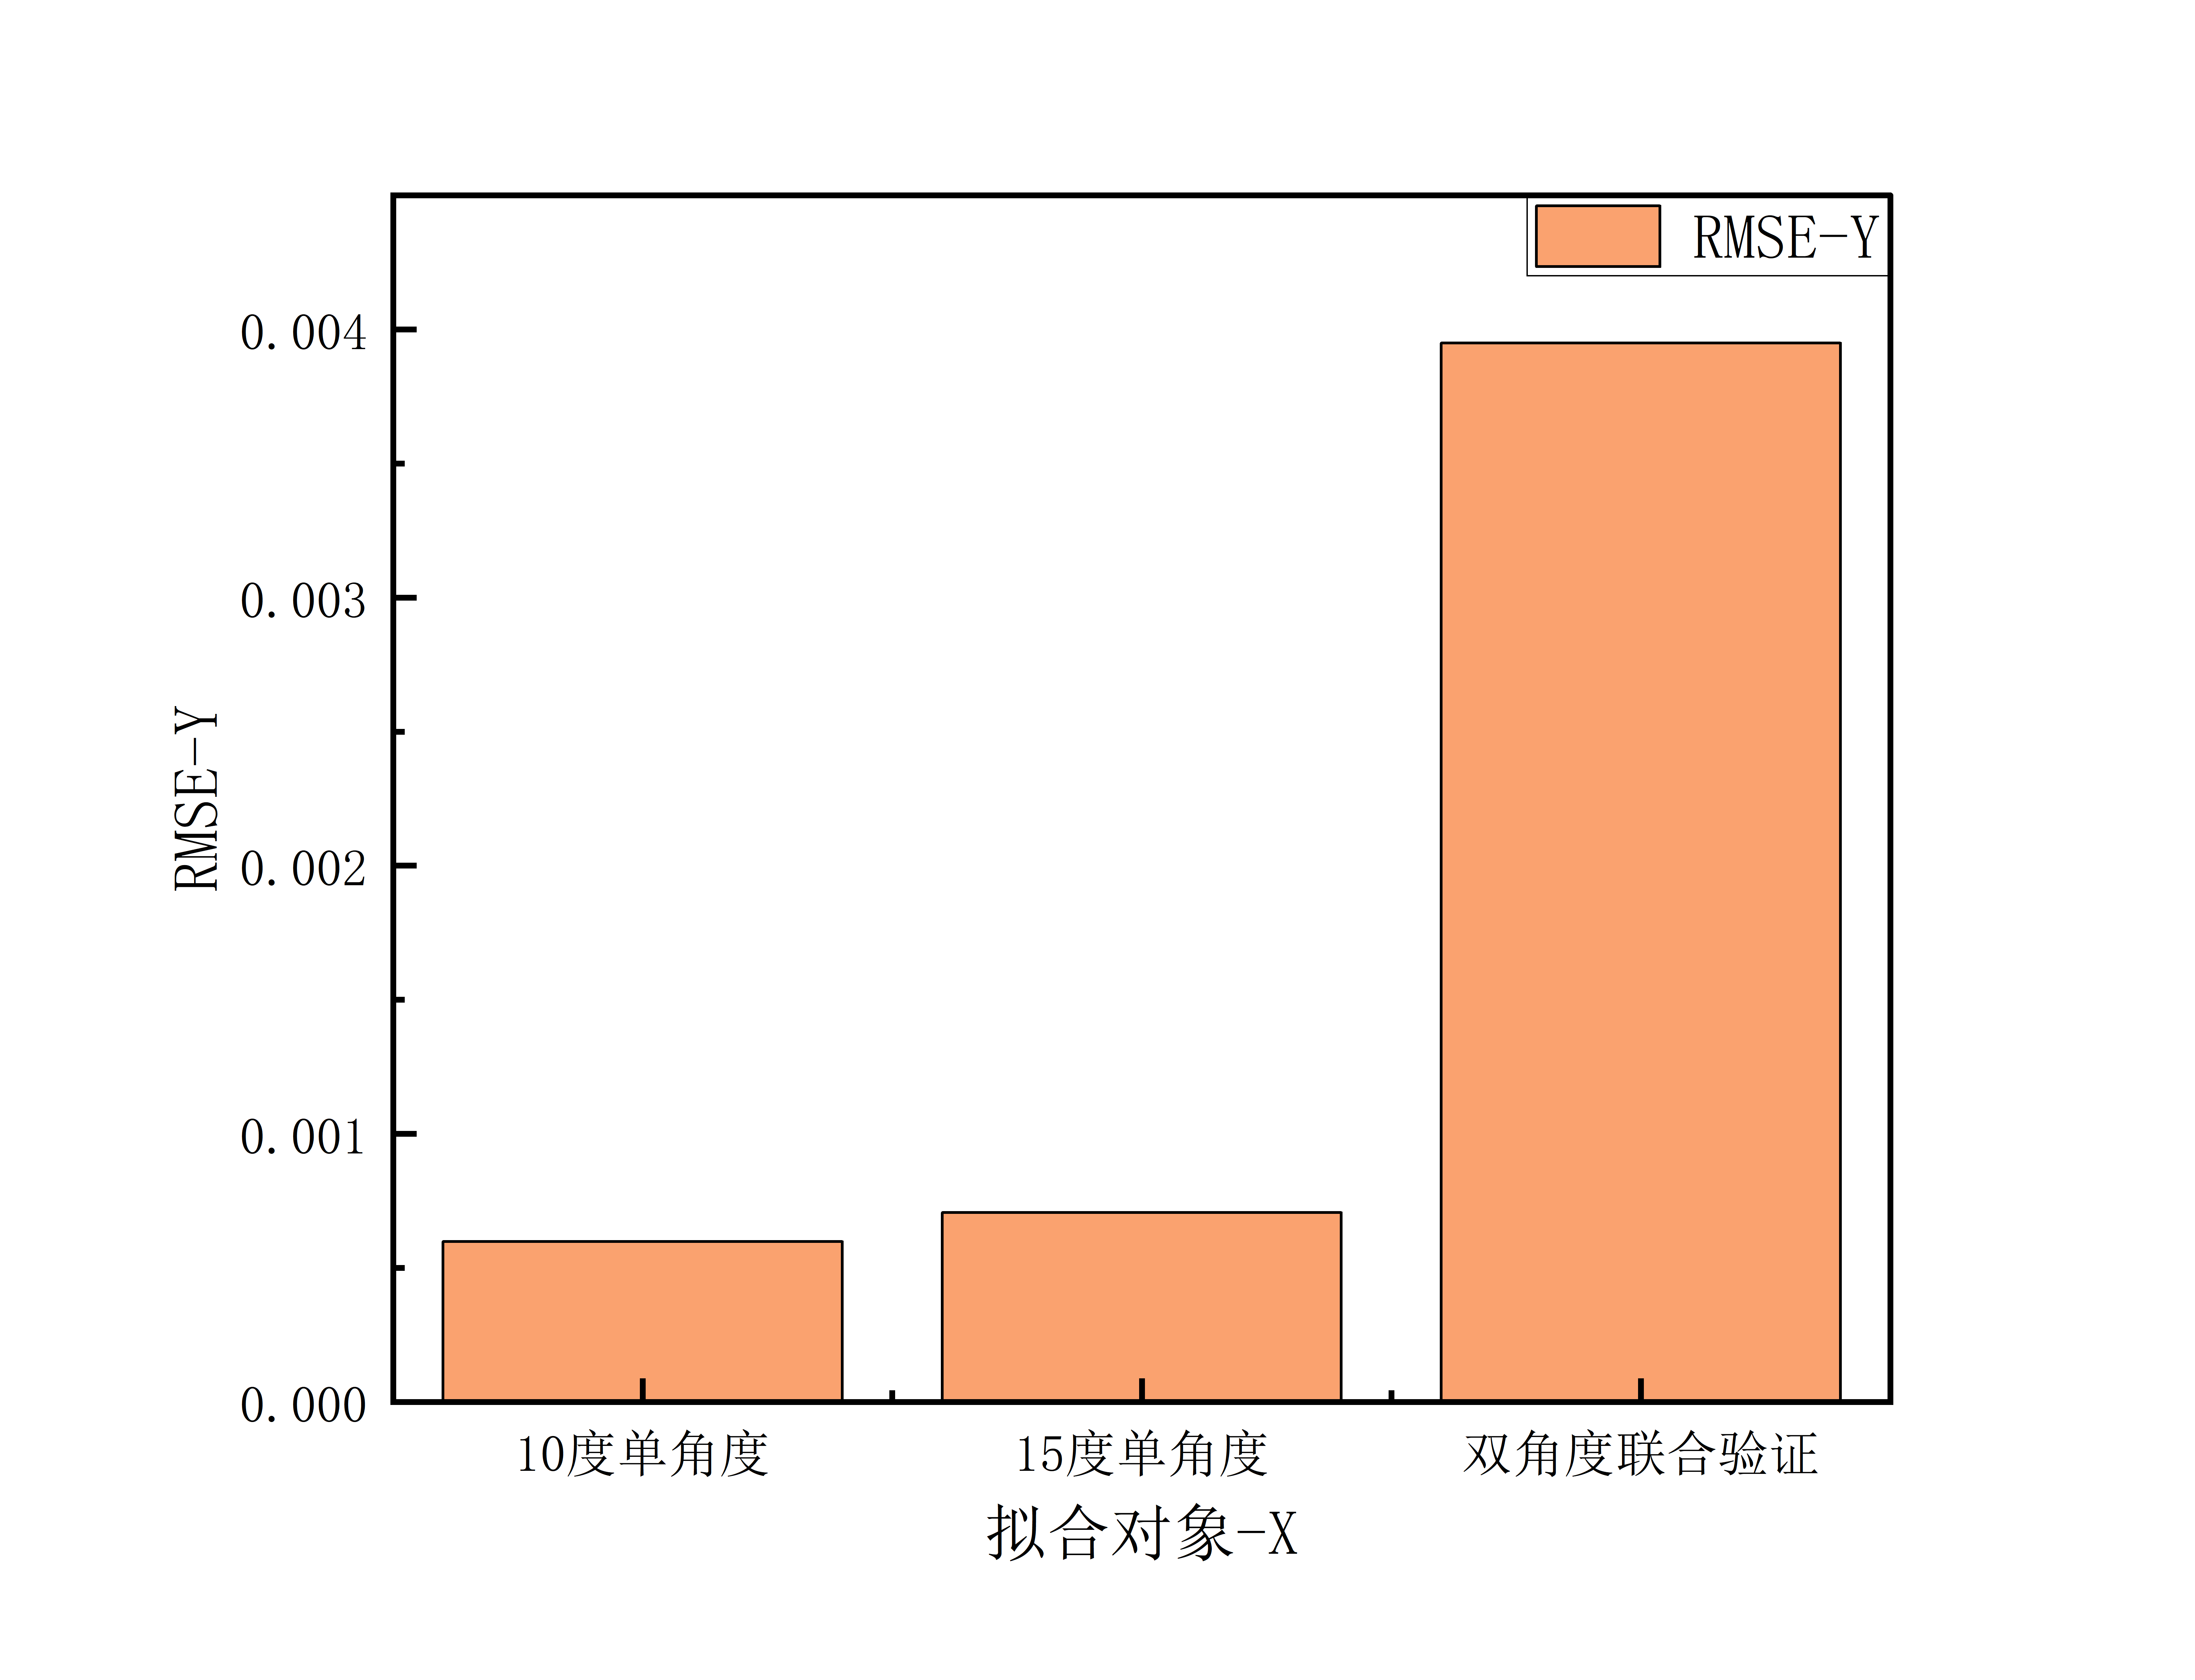
\includegraphics[width=\textwidth]{10_拟合RMSE柱状图.png}
			\caption{RMSE}
			\label{fig:rmse_bar}
		\end{subfigure}
		\hfill
		\begin{subfigure}[b]{0.31\textwidth}
			\centering
			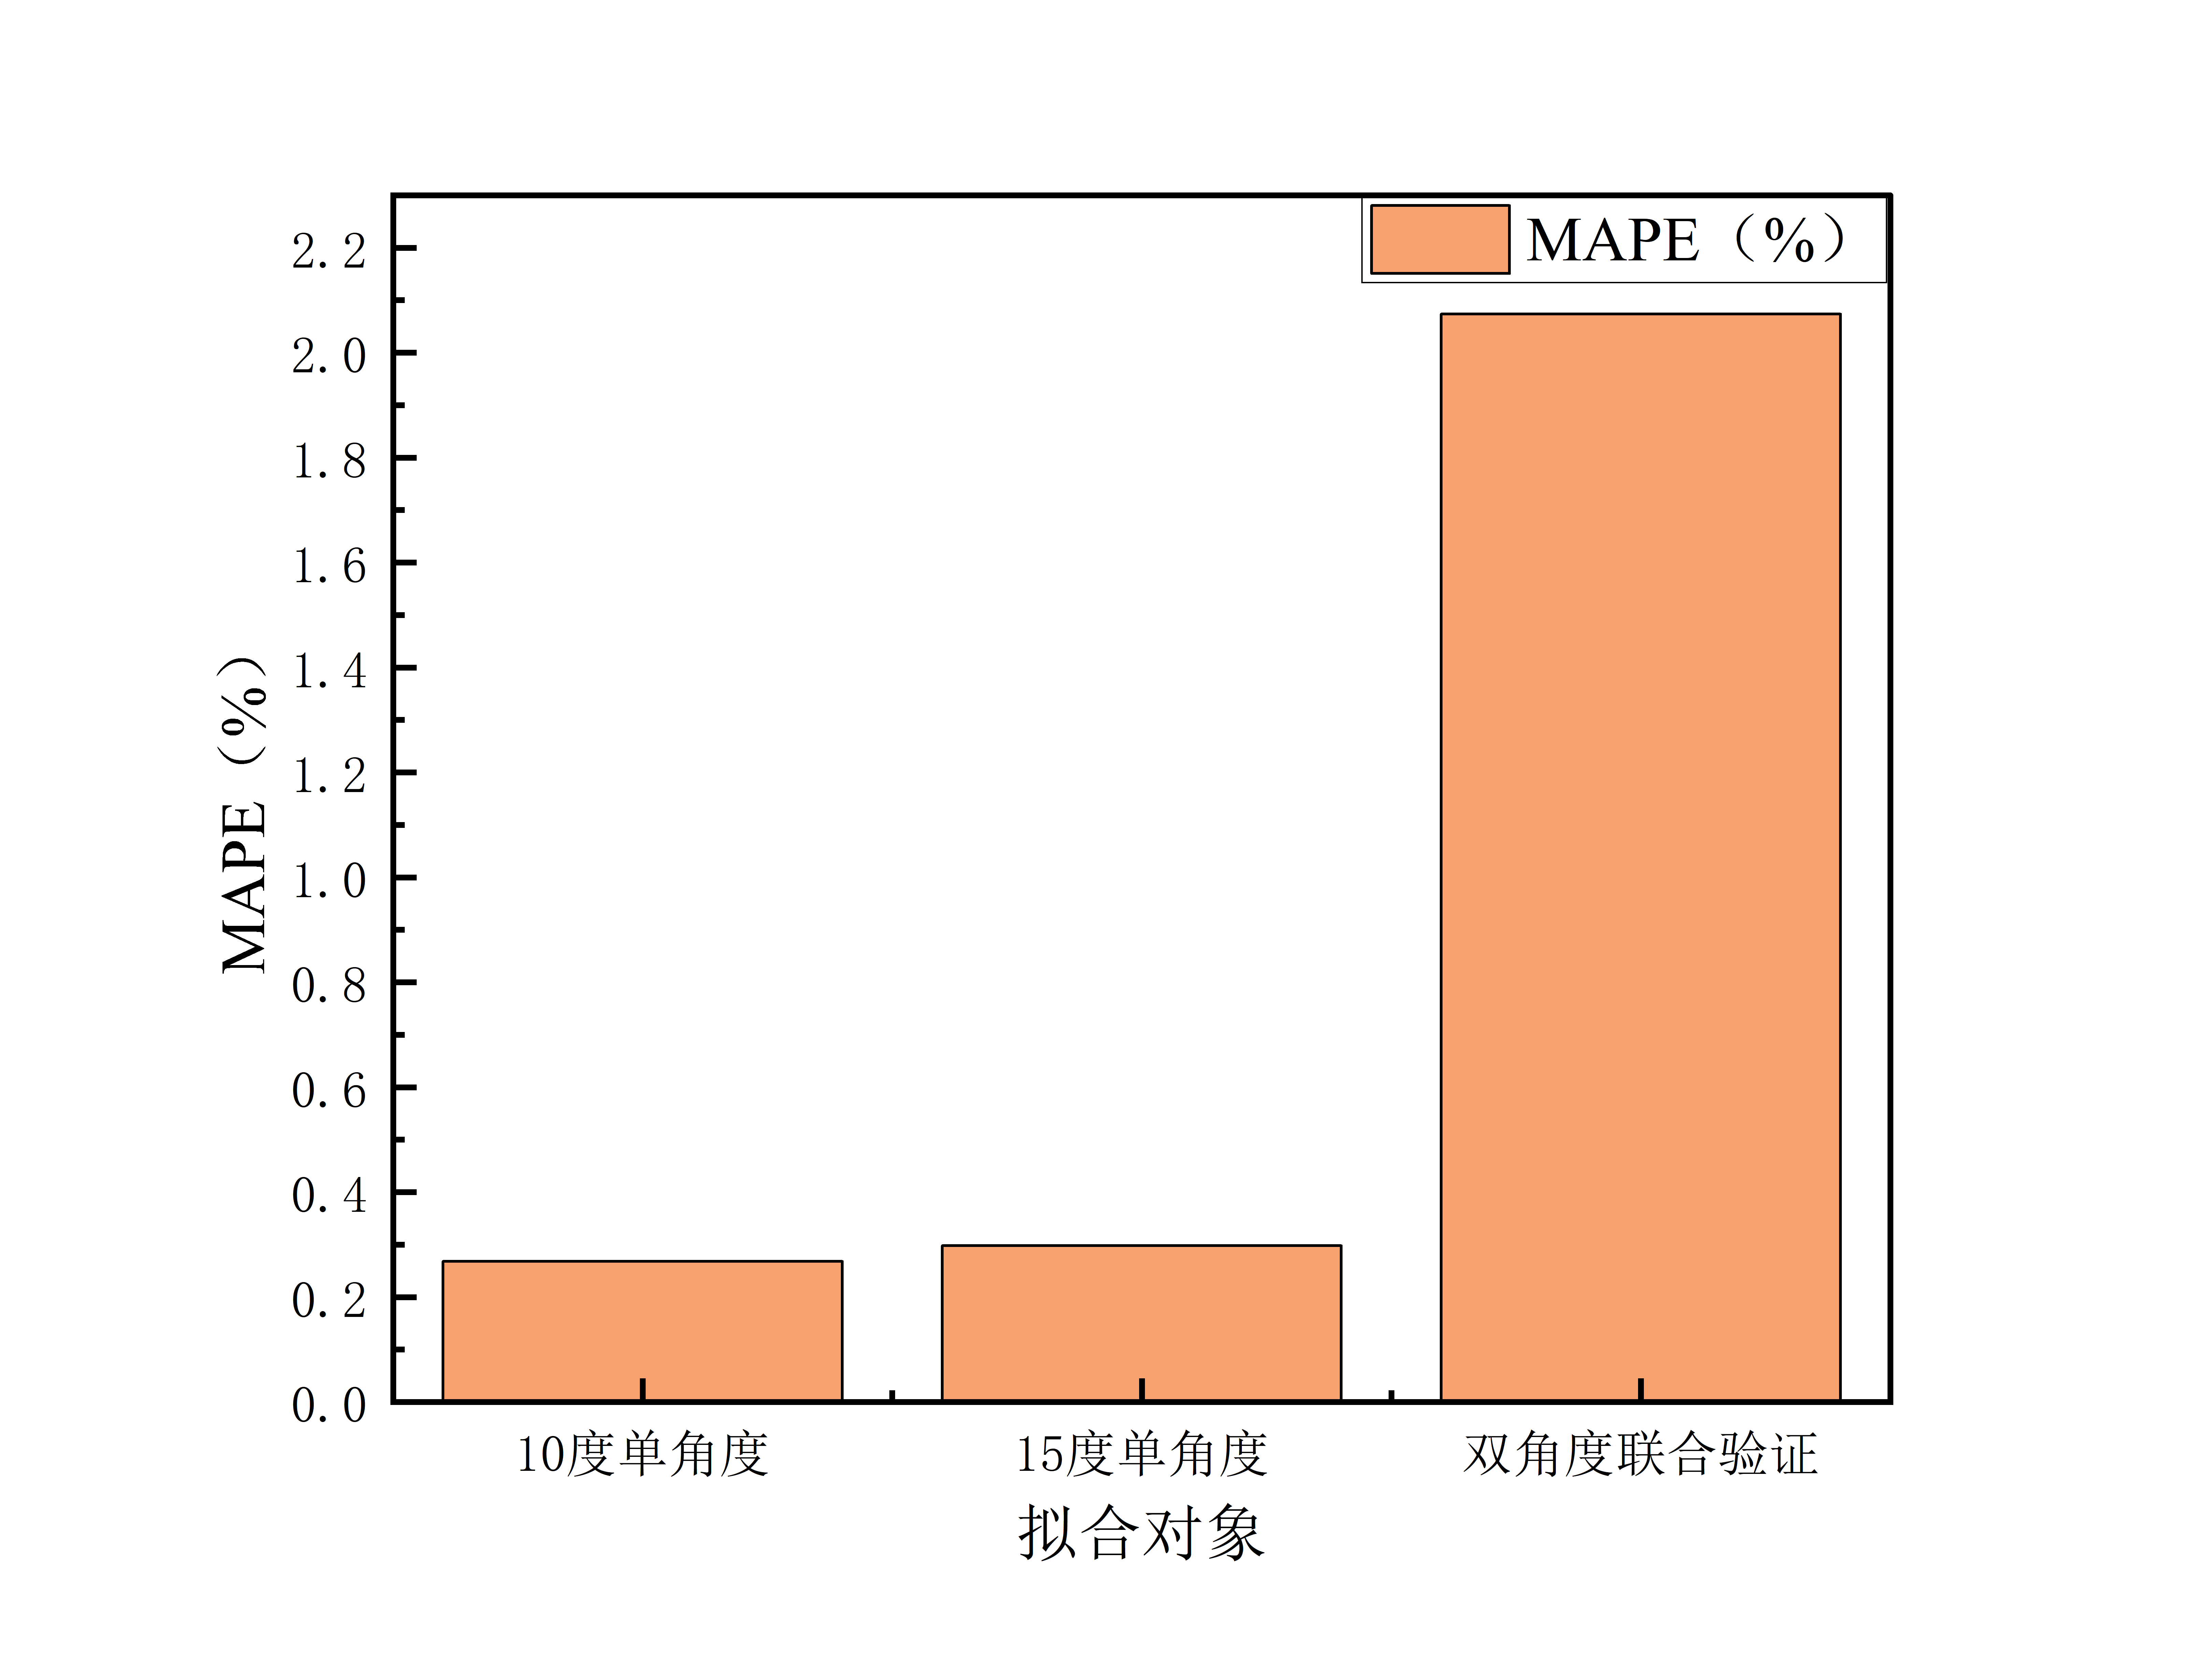
\includegraphics[width=\textwidth]{11_拟合MAPE柱状图.png}
			\caption{MAPE}
			\label{fig:mape_bar}
		\end{subfigure}
		\caption{厚度反演结果及拟合优度指标对比}
		\label{fig:thickness_metrics}
	\end{figure}
	
	\begin{figure}[htbp]
		\centering
		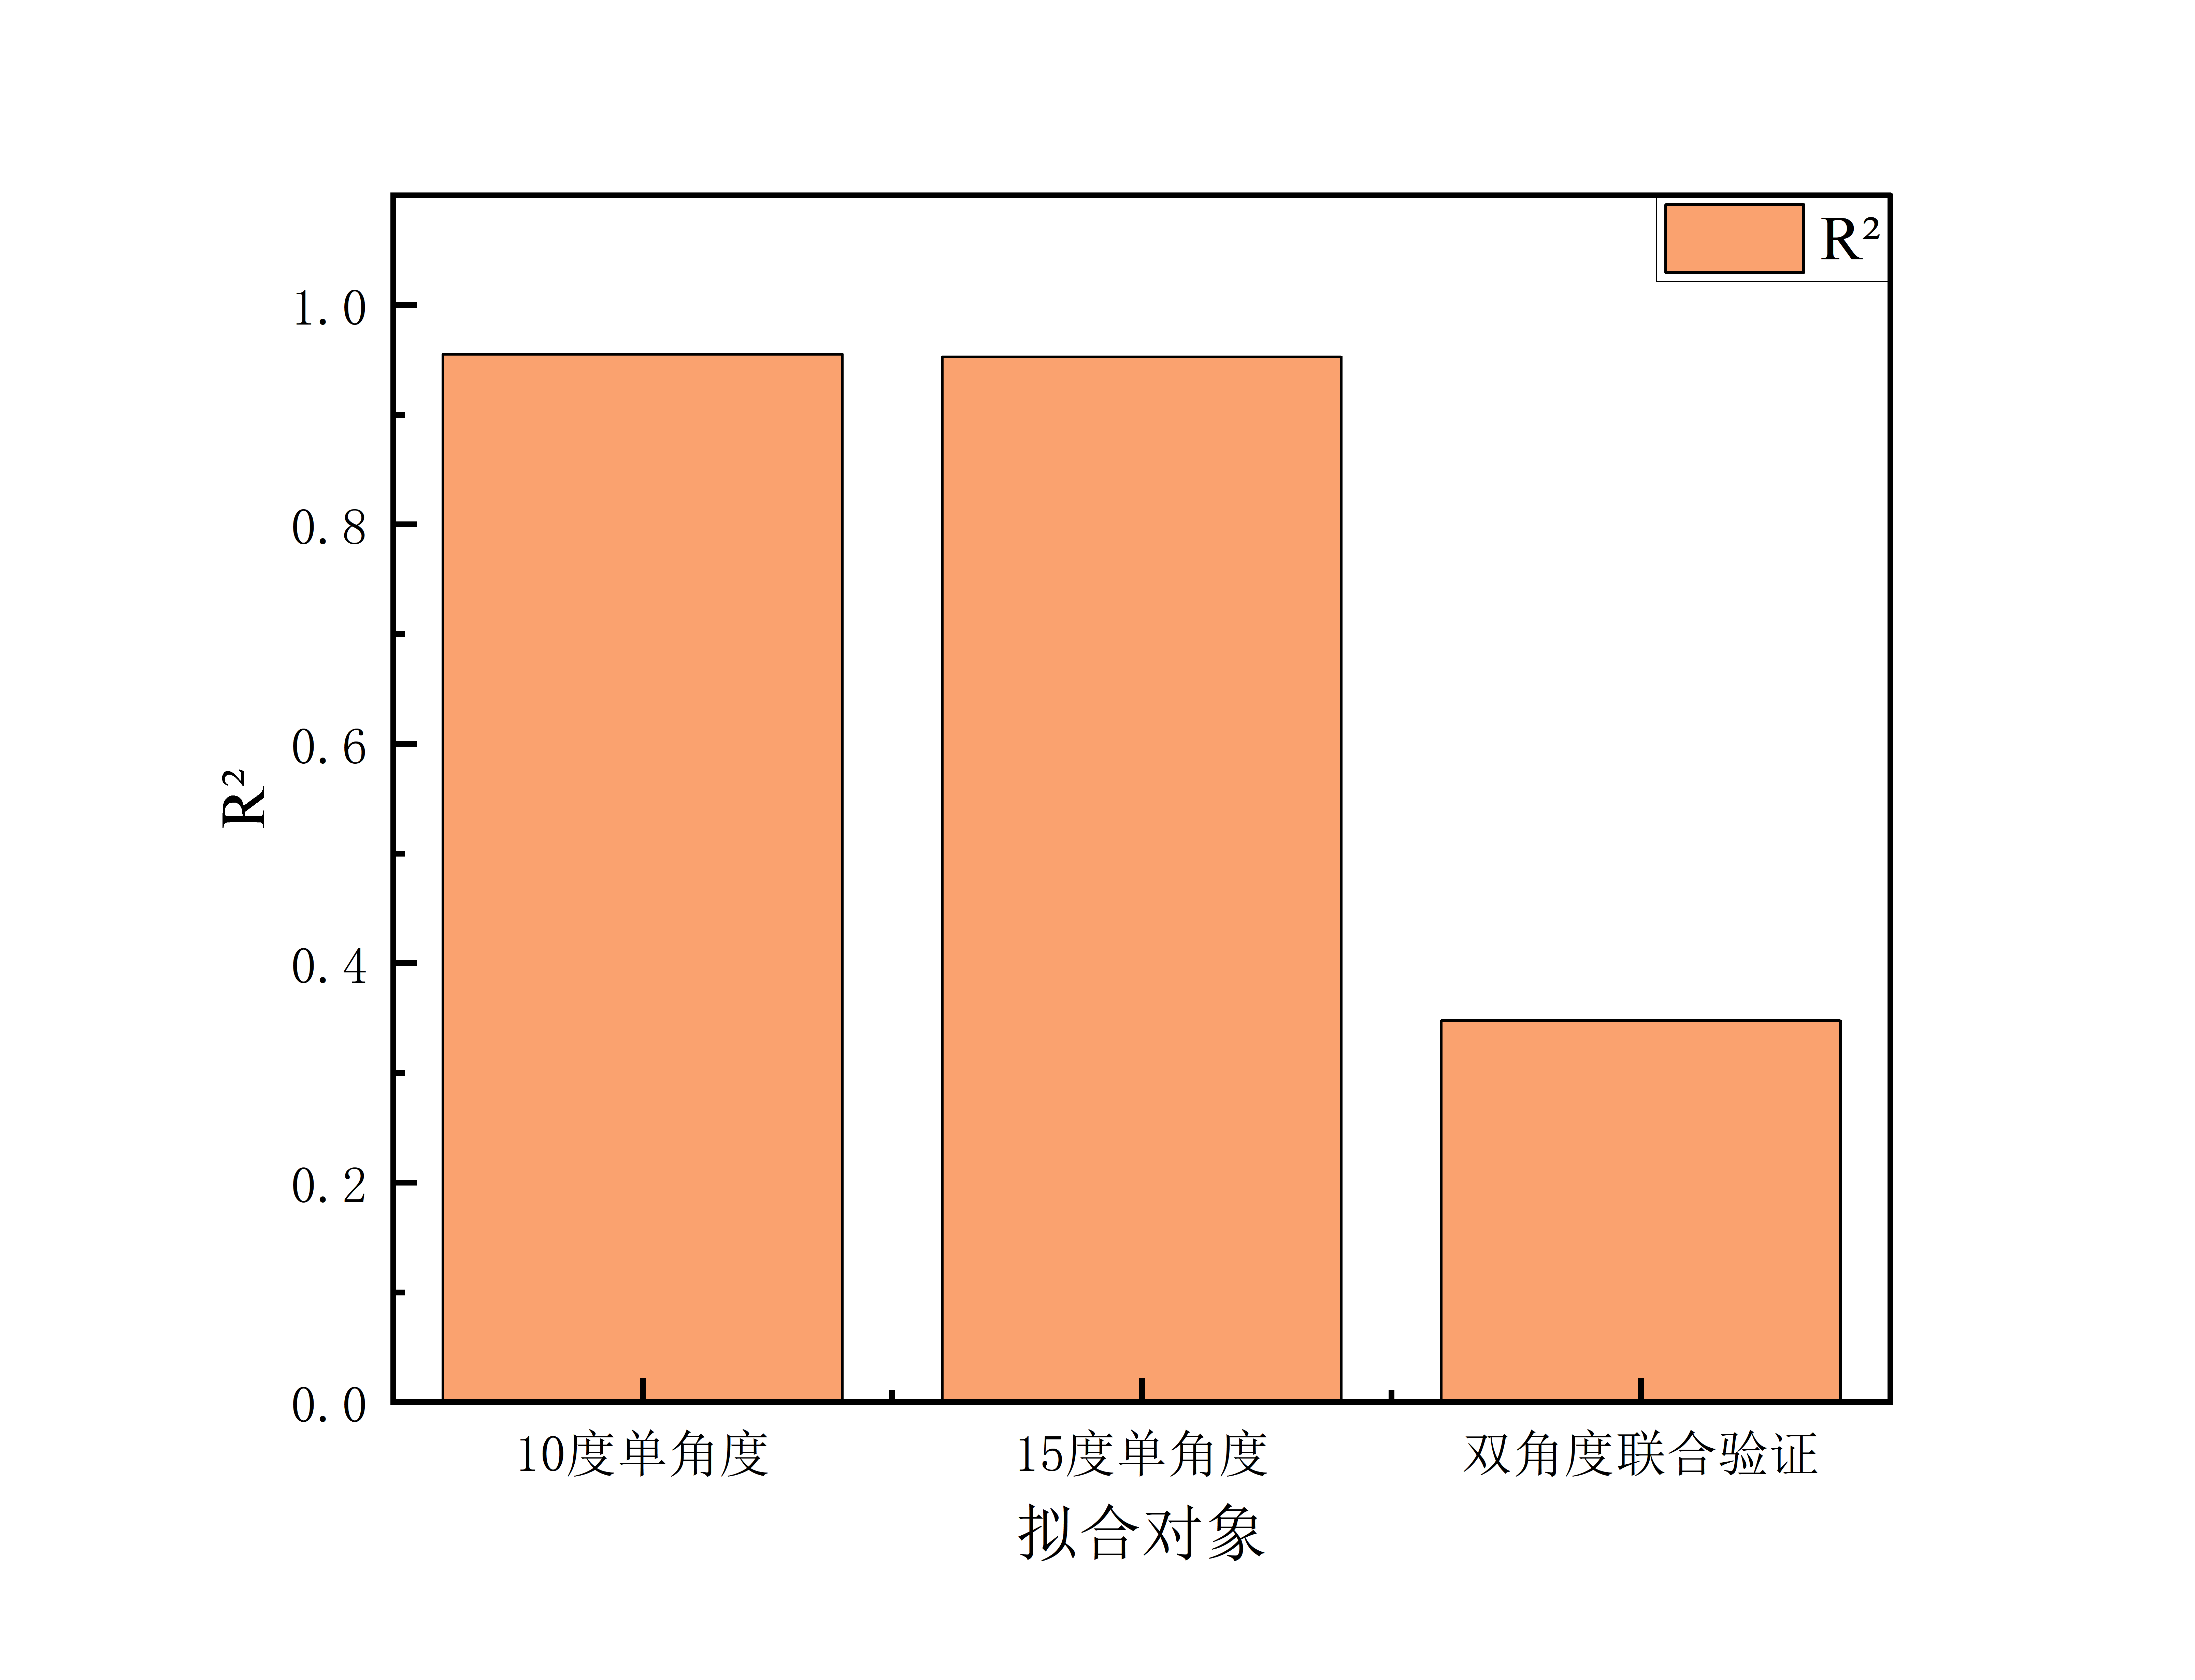
\includegraphics[width=0.5\textwidth]{12_拟合R2柱状图.png}
		\caption{拟合决定系数$R^2$柱状图}
		\label{fig:r2_bar}
	\end{figure}
	
	\subsubsection{多初值稳定性与残差正态性}
	
	为考察目标函数是否具有唯一的全局极小值，我们采用大量随机初值进行多次拟合，并将最终收敛的厚度值散点化，如图\ref{fig:multi_init_ecdf}所示。所有初值均收敛到 $7.7\sim7.9\ \mu\mathrm{m}$ 的狭窄区间内，未出现其他局部极小值吸引域，表明厚度参数具有良好的全局可辨识性。ECDF图进一步验证了残差的正态性假设——残差的经验累积分布与标准正态CDF高度重合，Kolmogorov–Smirnov检验$p>0.05$，满足最小二乘估计的基本假设。
	
	\begin{figure}[htbp]
		\centering
		\begin{subfigure}[b]{0.47\textwidth}
			\centering
			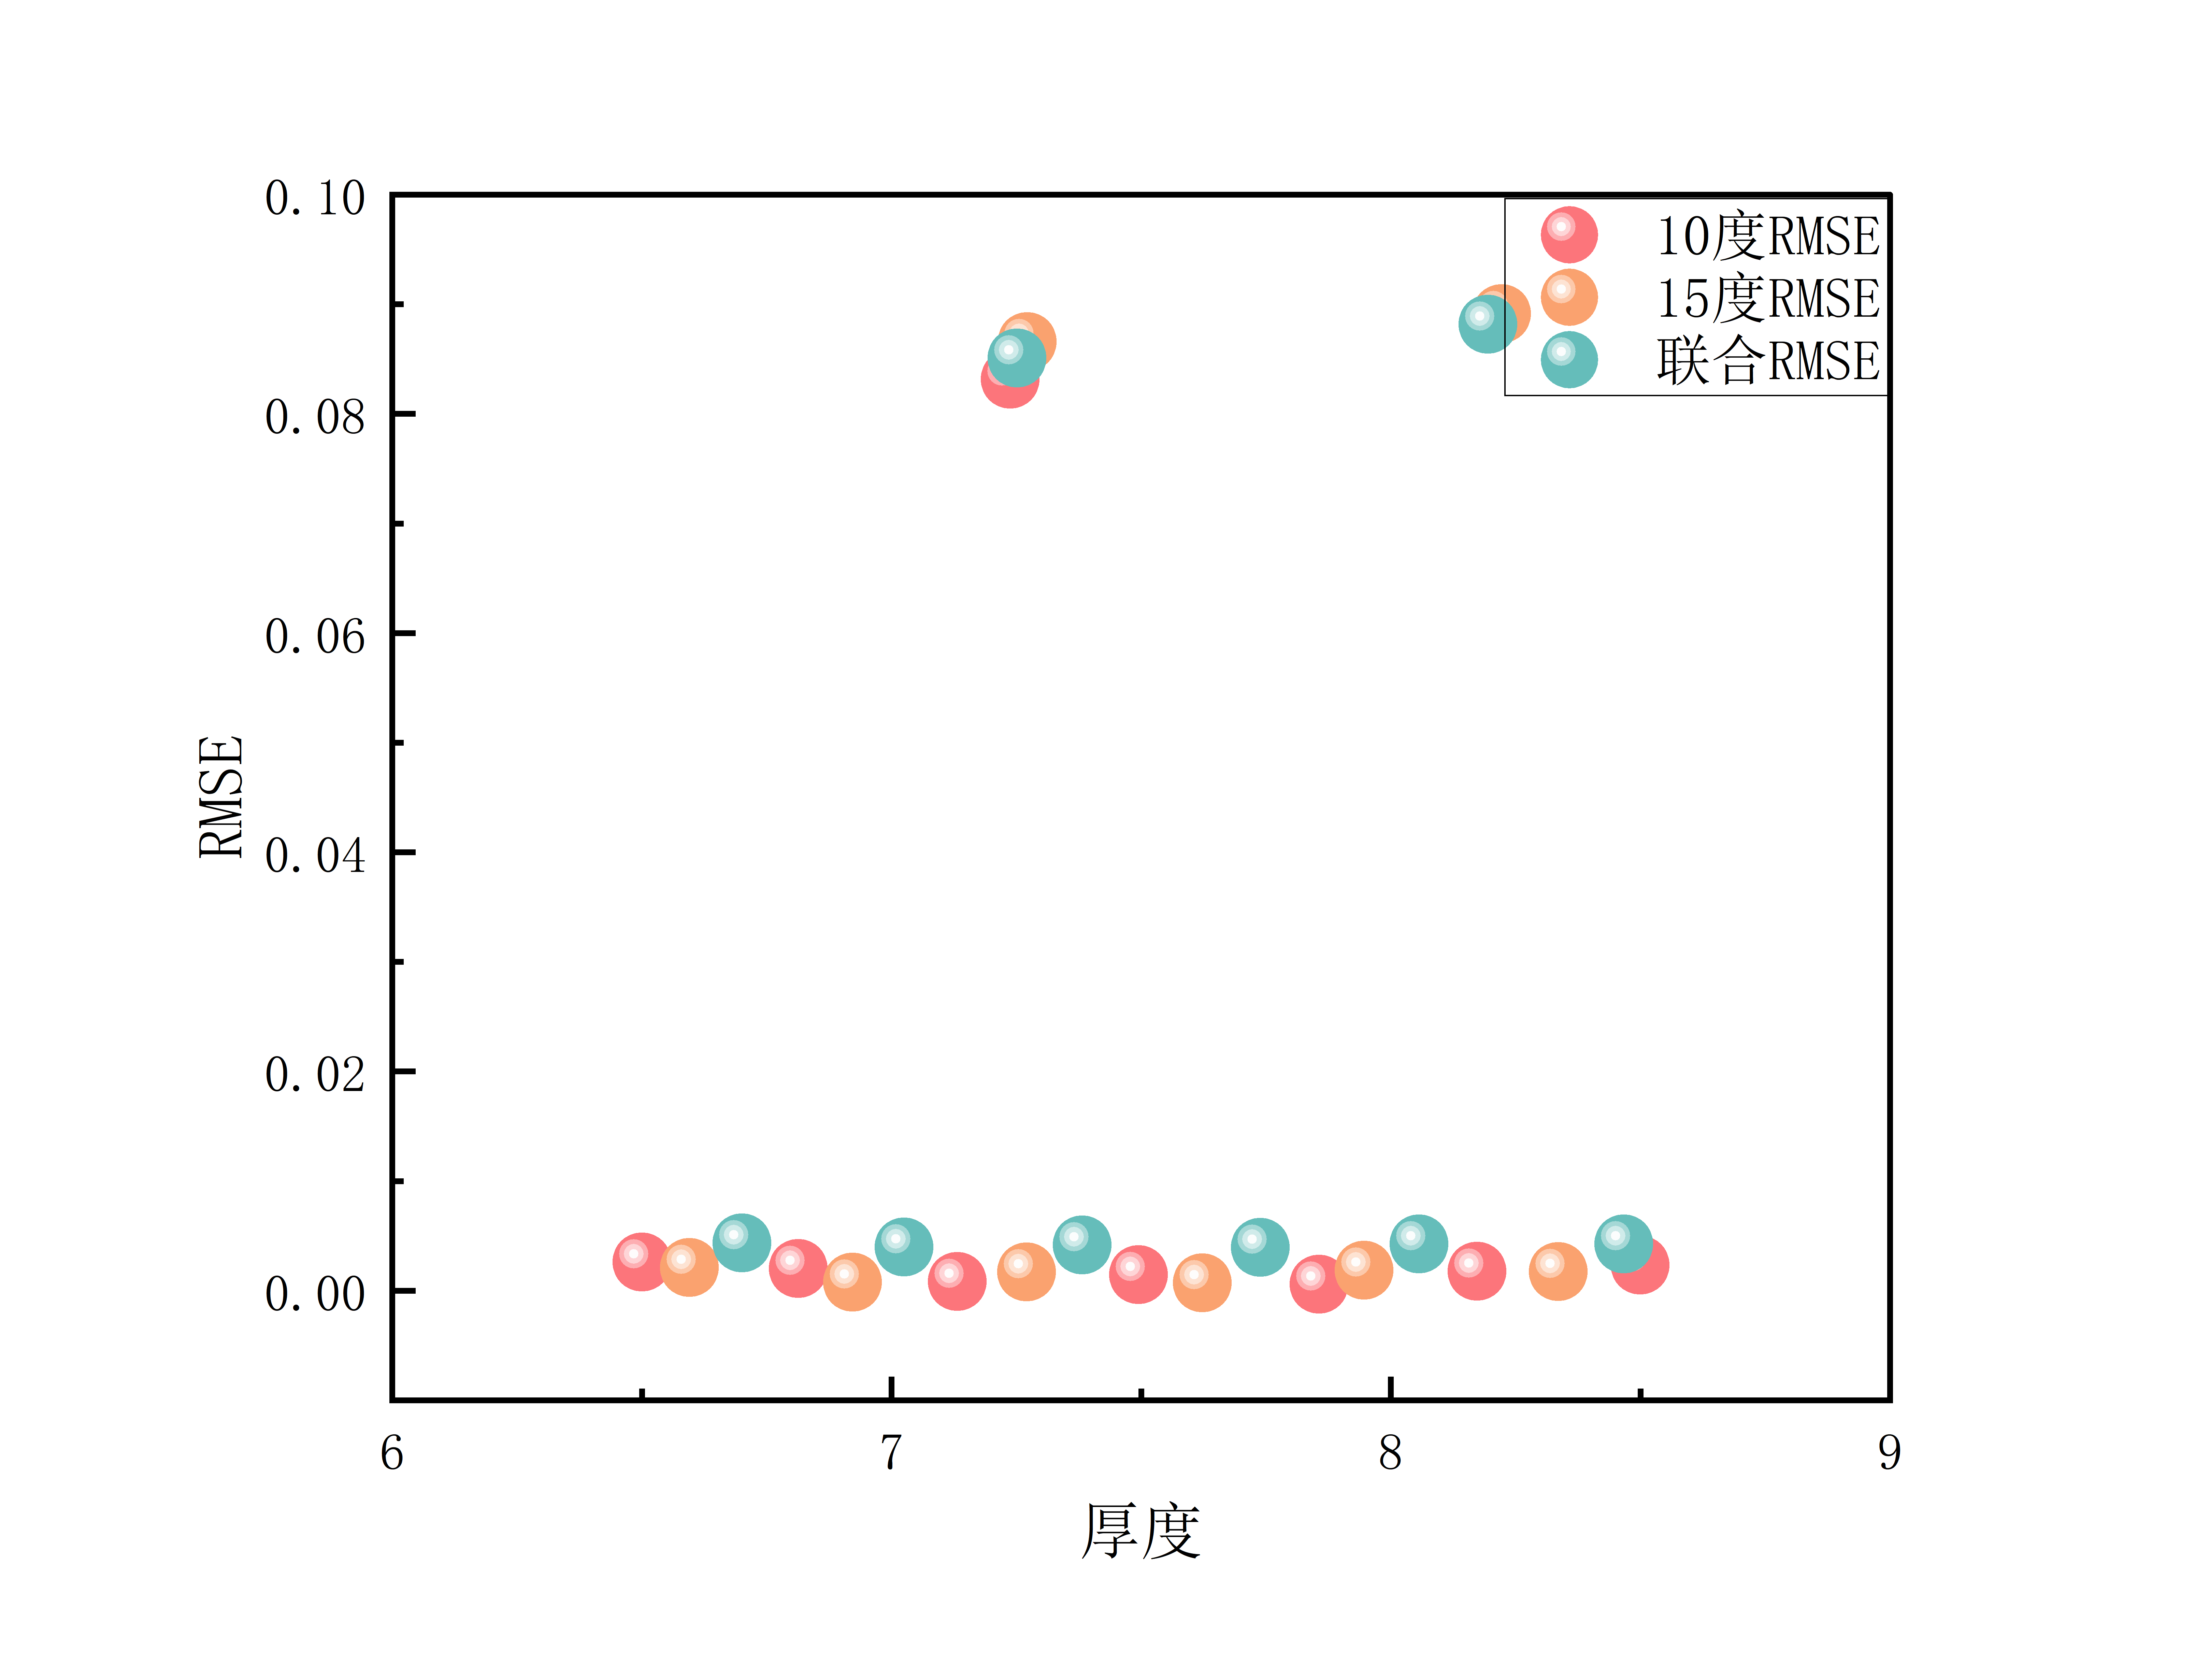
\includegraphics[width=\textwidth]{13_多初值稳定性散点.png}
			\caption{多初值收敛散点图}
			\label{fig:multi_init}
		\end{subfigure}
		\hfill
		\begin{subfigure}[b]{0.47\textwidth}
			\centering
			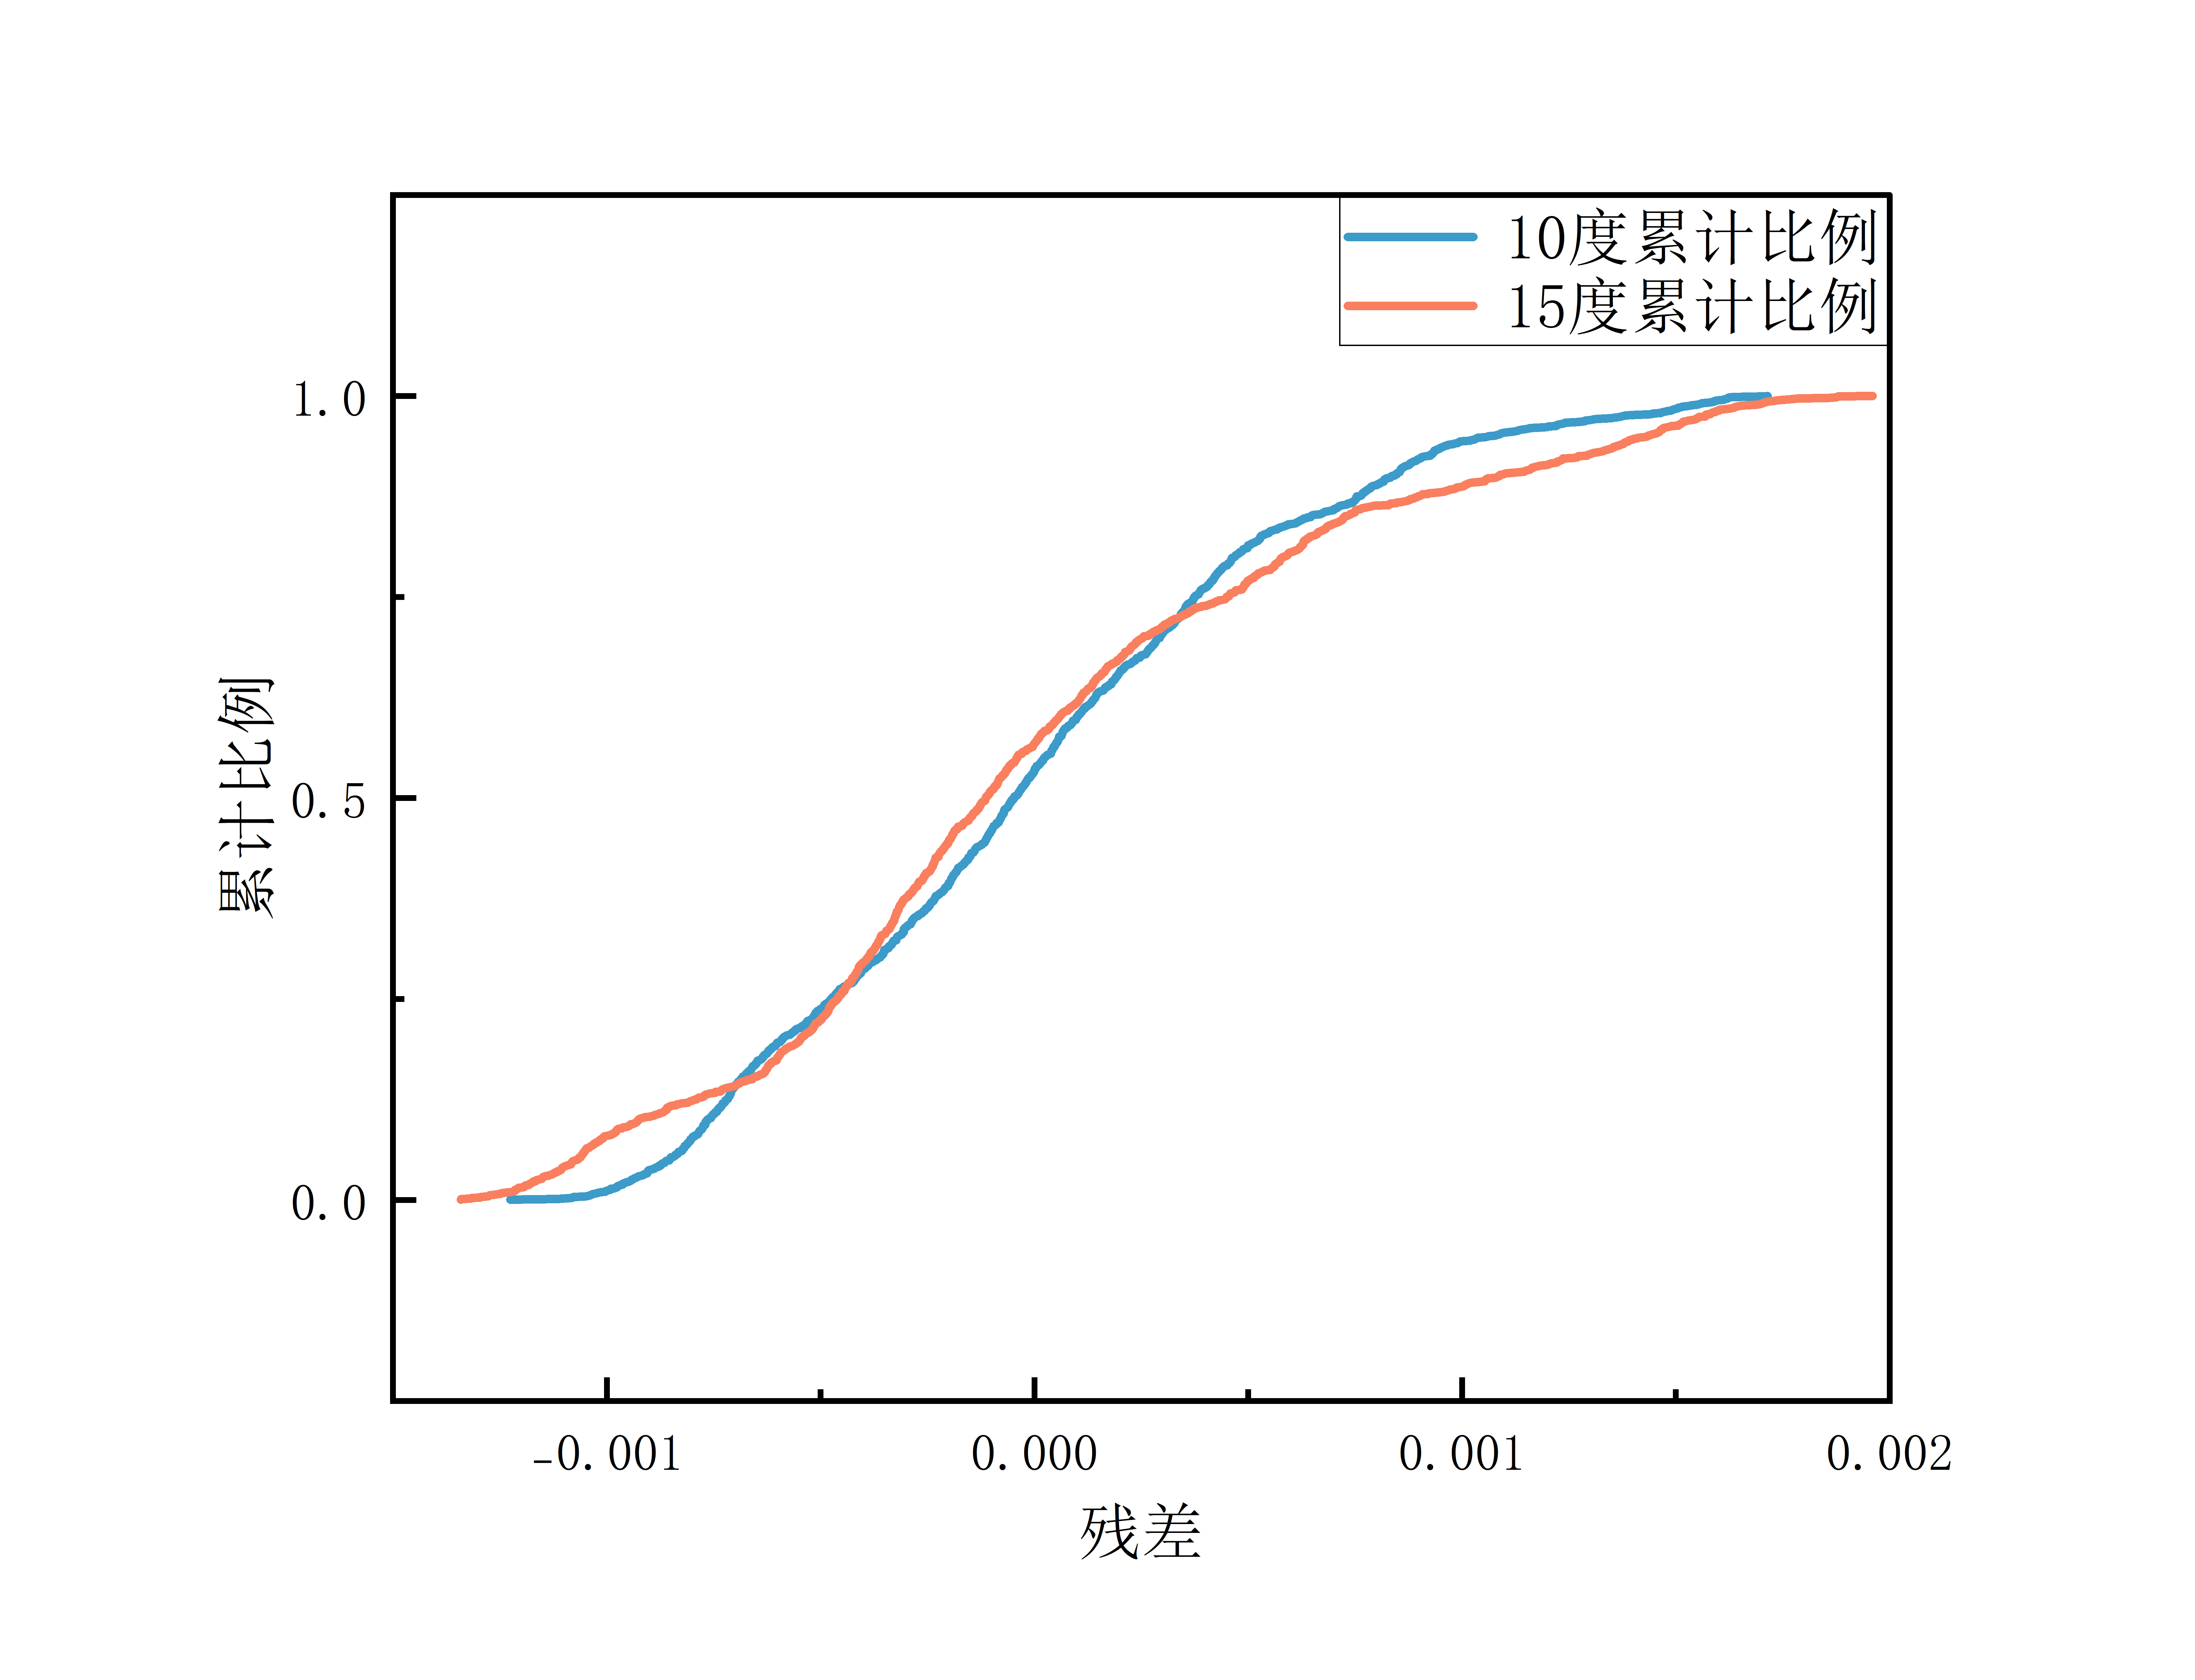
\includegraphics[width=\textwidth]{14_残差ECDF.png}
			\caption{残差ECDF与正态对比}
			\label{fig:resid_ecdf}
		\end{subfigure}
		\caption{多初值稳定性与残差正态性检验}
		\label{fig:multi_init_ecdf}
	\end{figure}
	
	\subsection{验证、灵敏度与局限性}
	
	两个角度的拟合曲线均复现实测峰谷位置，并落入同一条纹级次；独立厚度的相对差异为 $3.02\%$，支持以算术平均表示同一晶圆厚度。载流子浓度及若干Sellmeier扰动参数达到约束边界，说明这些附属参数在窄波段内不足以用于材料表征；它们只吸收谱形差异，不进入厚度结论。主厚度与PAPER\_A复现值一致，计算中未加入角度增益、偏置或共享参数联合拟合。
	
	\section{问题三模型的建立与求解}
	
	\subsection{问题三的描述与光谱特征}
	
	问题三要求讨论多光束干涉对测厚精度的影响，给出硅外延层厚度，并回溯检验问题二的SiC结果。硅在中红外波段具有明显吸收，不能沿用问题二的实折射率近似。本文以PAPER\_A为唯一主体：使用双振子-Drude复折射率和Airy无限多光束模型，对 $10^\circ$、$15^\circ$ 数据分别拟合后取平均。第三束光强比用于解释高阶光束量级，不再作为双光束与Airy之间的条件选择器。
	
	图\ref{fig:q3_concept}示意了Airy无限多光束模型的光路结构，与问题一的双光束模型不同，本图包含了表面反射光$E_1$、第一束内部反射光$E_2$、第二束内部反射光$E_3$以及后续高阶反射光的级联叠加。硅外延层在中红外波段的吸收由复折射率$\widetilde n_2$描述，传播因子$P=\exp(-i4\pi\sigma d\widetilde n_2\cos\gamma)$包含衰减。
	
	\begin{figure}[htbp]
		\centering
		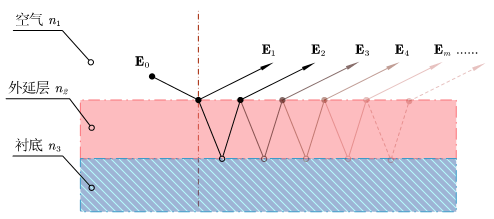
\includegraphics[width=1.0\textwidth]{q3_concept.png}
		\caption{空气-硅外延层-衬底三层结构中的多光束干涉光路示意图}
		\label{fig:q3_concept}
	\end{figure}
	
	\subsection{硅双振子-Drude复折射率}
	
	令 $\lambda=10^4/\sigma$，硅的晶格介电函数为
	\begin{equation}
		\widetilde{\epsilon}_{\mathrm L}(\lambda) = \epsilon_\infty + \sum_{j=1}^{2} \frac{A_j\lambda^2}{\lambda^2 - \lambda_j^2 + i\Gamma_j\lambda},
	\end{equation}
	其中 $\epsilon_\infty=11.68$，$(A_1,A_2)=(0.29972,11.34965)$，$(\lambda_1,\lambda_2)=(10.6683,16.2026)\ \mu\mathrm{m}$，$(\Gamma_1,\Gamma_2)=(0.092613,0.23572)\ \mu\mathrm{m}$。自由载流子项为
	\begin{equation}
		\widetilde{\epsilon}_{\mathrm D} = -\frac{\omega_p^2}{\omega^2 - i\Gamma_e\omega},\qquad
		\omega_p^2 = \frac{Ne^2}{\epsilon_0(0.26m_0)},
	\end{equation}
	并令 $\widetilde n_2^2 = \widetilde{\epsilon}_{\mathrm L} + \widetilde{\epsilon}_{\mathrm D}$。全文采用 $\exp(-ikz)$ 约定，选择 $\operatorname{Im}\widetilde n_2\le0$ 的平方根支路，以保证传播衰减。
	
	\subsection{第三束光强比与Airy模型}
	
	折射角采用PAPER\_A的实角近似
	\begin{equation}
		\gamma = \arcsin\left(\frac{n_1\sin i}{\operatorname{Re}\widetilde n_2}\right),
	\end{equation}
	而完整复折射率仍代入$s$、$p$偏振Fresnel系数。外延层一次往返传播因子为
	\begin{equation}
		P = \exp\left(-i4\pi\times10^{-4}\sigma d\,\widetilde n_2\cos\gamma\right),
	\end{equation}
	程序逐点验证 $0<|P|\le1$。对偏振态 $u$，前三束反射场写为
	\begin{equation}
		E_1^{(u)} = r_{12}^{(u)}E_0,\qquad
		E_2^{(u)} = t_{12}^{(u)}r_{23}^{(u)}t_{21}^{(u)}P E_0,
	\end{equation}
	\begin{equation}
		E_3^{(u)} = t_{12}^{(u)}r_{23}^{(u)}r_{21}^{(u)}r_{23}^{(u)}t_{21}^{(u)}P^2 E_0.
	\end{equation}
	第三束相对表面反射束的强度比定义为
	\begin{equation}
		\eta_3 = \frac{|E_3^{(s)}|^2 + |E_3^{(p)}|^2}{|E_1^{(s)}|^2 + |E_1^{(p)}|^2},
	\end{equation}
	并以 $0.1\%$ 作为工程参照阈值。硅的正式反射振幅始终采用
	\begin{equation}
		\rho_{\mathrm{Airy}}^{(u)} = r_{12}^{(u)} + \frac{t_{12}^{(u)}t_{21}^{(u)}r_{23}^{(u)}P}{1 - r_{21}^{(u)}r_{23}^{(u)}P},
	\end{equation}
	非偏振反射率为 $R_{\mathrm{Airy}} = (|\rho_{\mathrm{Airy}}^{(s)}|^2 + |\rho_{\mathrm{Airy}}^{(p)}|^2)/2$。
	
	\subsection{硅分角度Airy反演}
	
	删除附件3、4的共同零值边界点，在 $1500\sim3500\ \mathrm{cm^{-1}}$ 内分别拟合
	\begin{equation}
		\mathbf{p}_k = (d_k, n_{3,k}, \log_{10}N_k, \log_{10}\Gamma_{e,k}),
	\end{equation}
	固定式(14)的背景参数和有效质量，不引入角度增益、偏置或共享参数联合拟合。每个角度采用确定性多初值有界最小二乘，厚度主结果为两个单角度解的算术平均。
	
	图\ref{fig:q3_flow}给出了上述反演流程的完整结构，分为两条主线：左侧为硅外延层Airy反演，右侧为SiC回溯检验，两条主线在最终厚度判定处汇合。
	
	\begin{figure}[htbp]
		\centering
		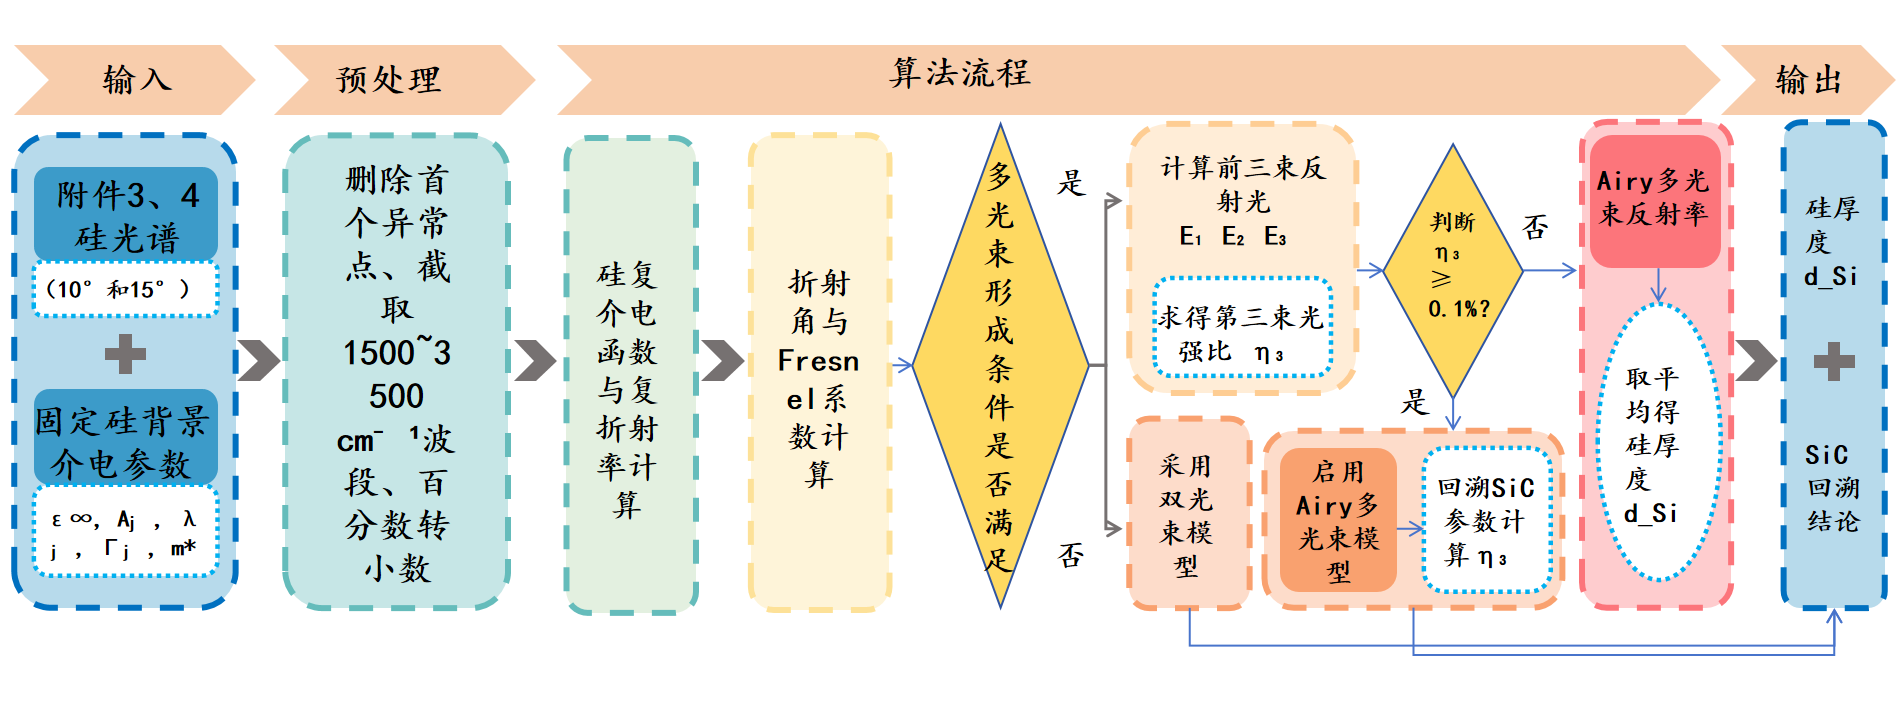
\includegraphics[width=1.0\textwidth]{3.png}
		\caption{问题三固定背景四参数Airy反演与SiC回溯检验的完整流程图}
		\label{fig:q3_flow}
	\end{figure}
	
	\subsection{硅重算结果与模型诊断}
	
	严格固定背景参数后，两个角度的Airy厚度分别为
	\begin{equation}
		d_{10^\circ}^{\mathrm{Si}} = 3.2480\ \mu\mathrm{m},\qquad
		d_{15^\circ}^{\mathrm{Si}} = 3.1875\ \mu\mathrm{m},
	\end{equation}
	算术平均为
	\begin{equation}
		\boxed{d_{\mathrm{Si}} = 3.2178\ \mu\mathrm{m}.}
	\end{equation}
	
	两角度RMSE分别为 $1.8738$ 和 $3.3554$ 个反射率百分点。该均值较PAPER\_A报告的 $3.040\ \mu\mathrm{m}$ 高 $5.85\%$。波段、单位、反射率缩放、参数边界和传播衰减检查均通过；差异来自参数口径：本文固定振子参数与有效质量，只拟合 $d$、$n_3$、$N$ 和 $\Gamma_e$，而范文附录的最终阶段重新释放了部分背景量。本文不以增加弱可辨识参数换取数值贴合，故将 $3.2178\ \mu\mathrm{m}$ 冻结为诚实重算结果，并把 $5.85\%$ 差异一并报告。
	
	\subsubsection{双角度拟合曲线与残差分析}
	
	图\ref{fig:si_fit_band}展示了硅外延层在 $10^\circ$ 和 $15^\circ$ 两个入射角下的Airy模型拟合结果。图中蓝色带状区域表示拟合曲线的置信区间，红色散点为实测反射率数据。可以看出，模型在两个角度下均能较好地捕捉光谱的主要振荡特征，峰谷位置与实测数据吻合良好。$10^\circ$ 入射角的拟合残差整体较小且分布均匀，而 $15^\circ$ 入射角在部分波数区间（如 $2800\sim3000\ \mathrm{cm^{-1}}$）残差有所增大，这反映了大角度下干涉条纹对厚度变化更为敏感，同时也说明硅衬底吸收在该波段的影响不可忽略。
	
	\begin{figure}[htbp]
		\centering
		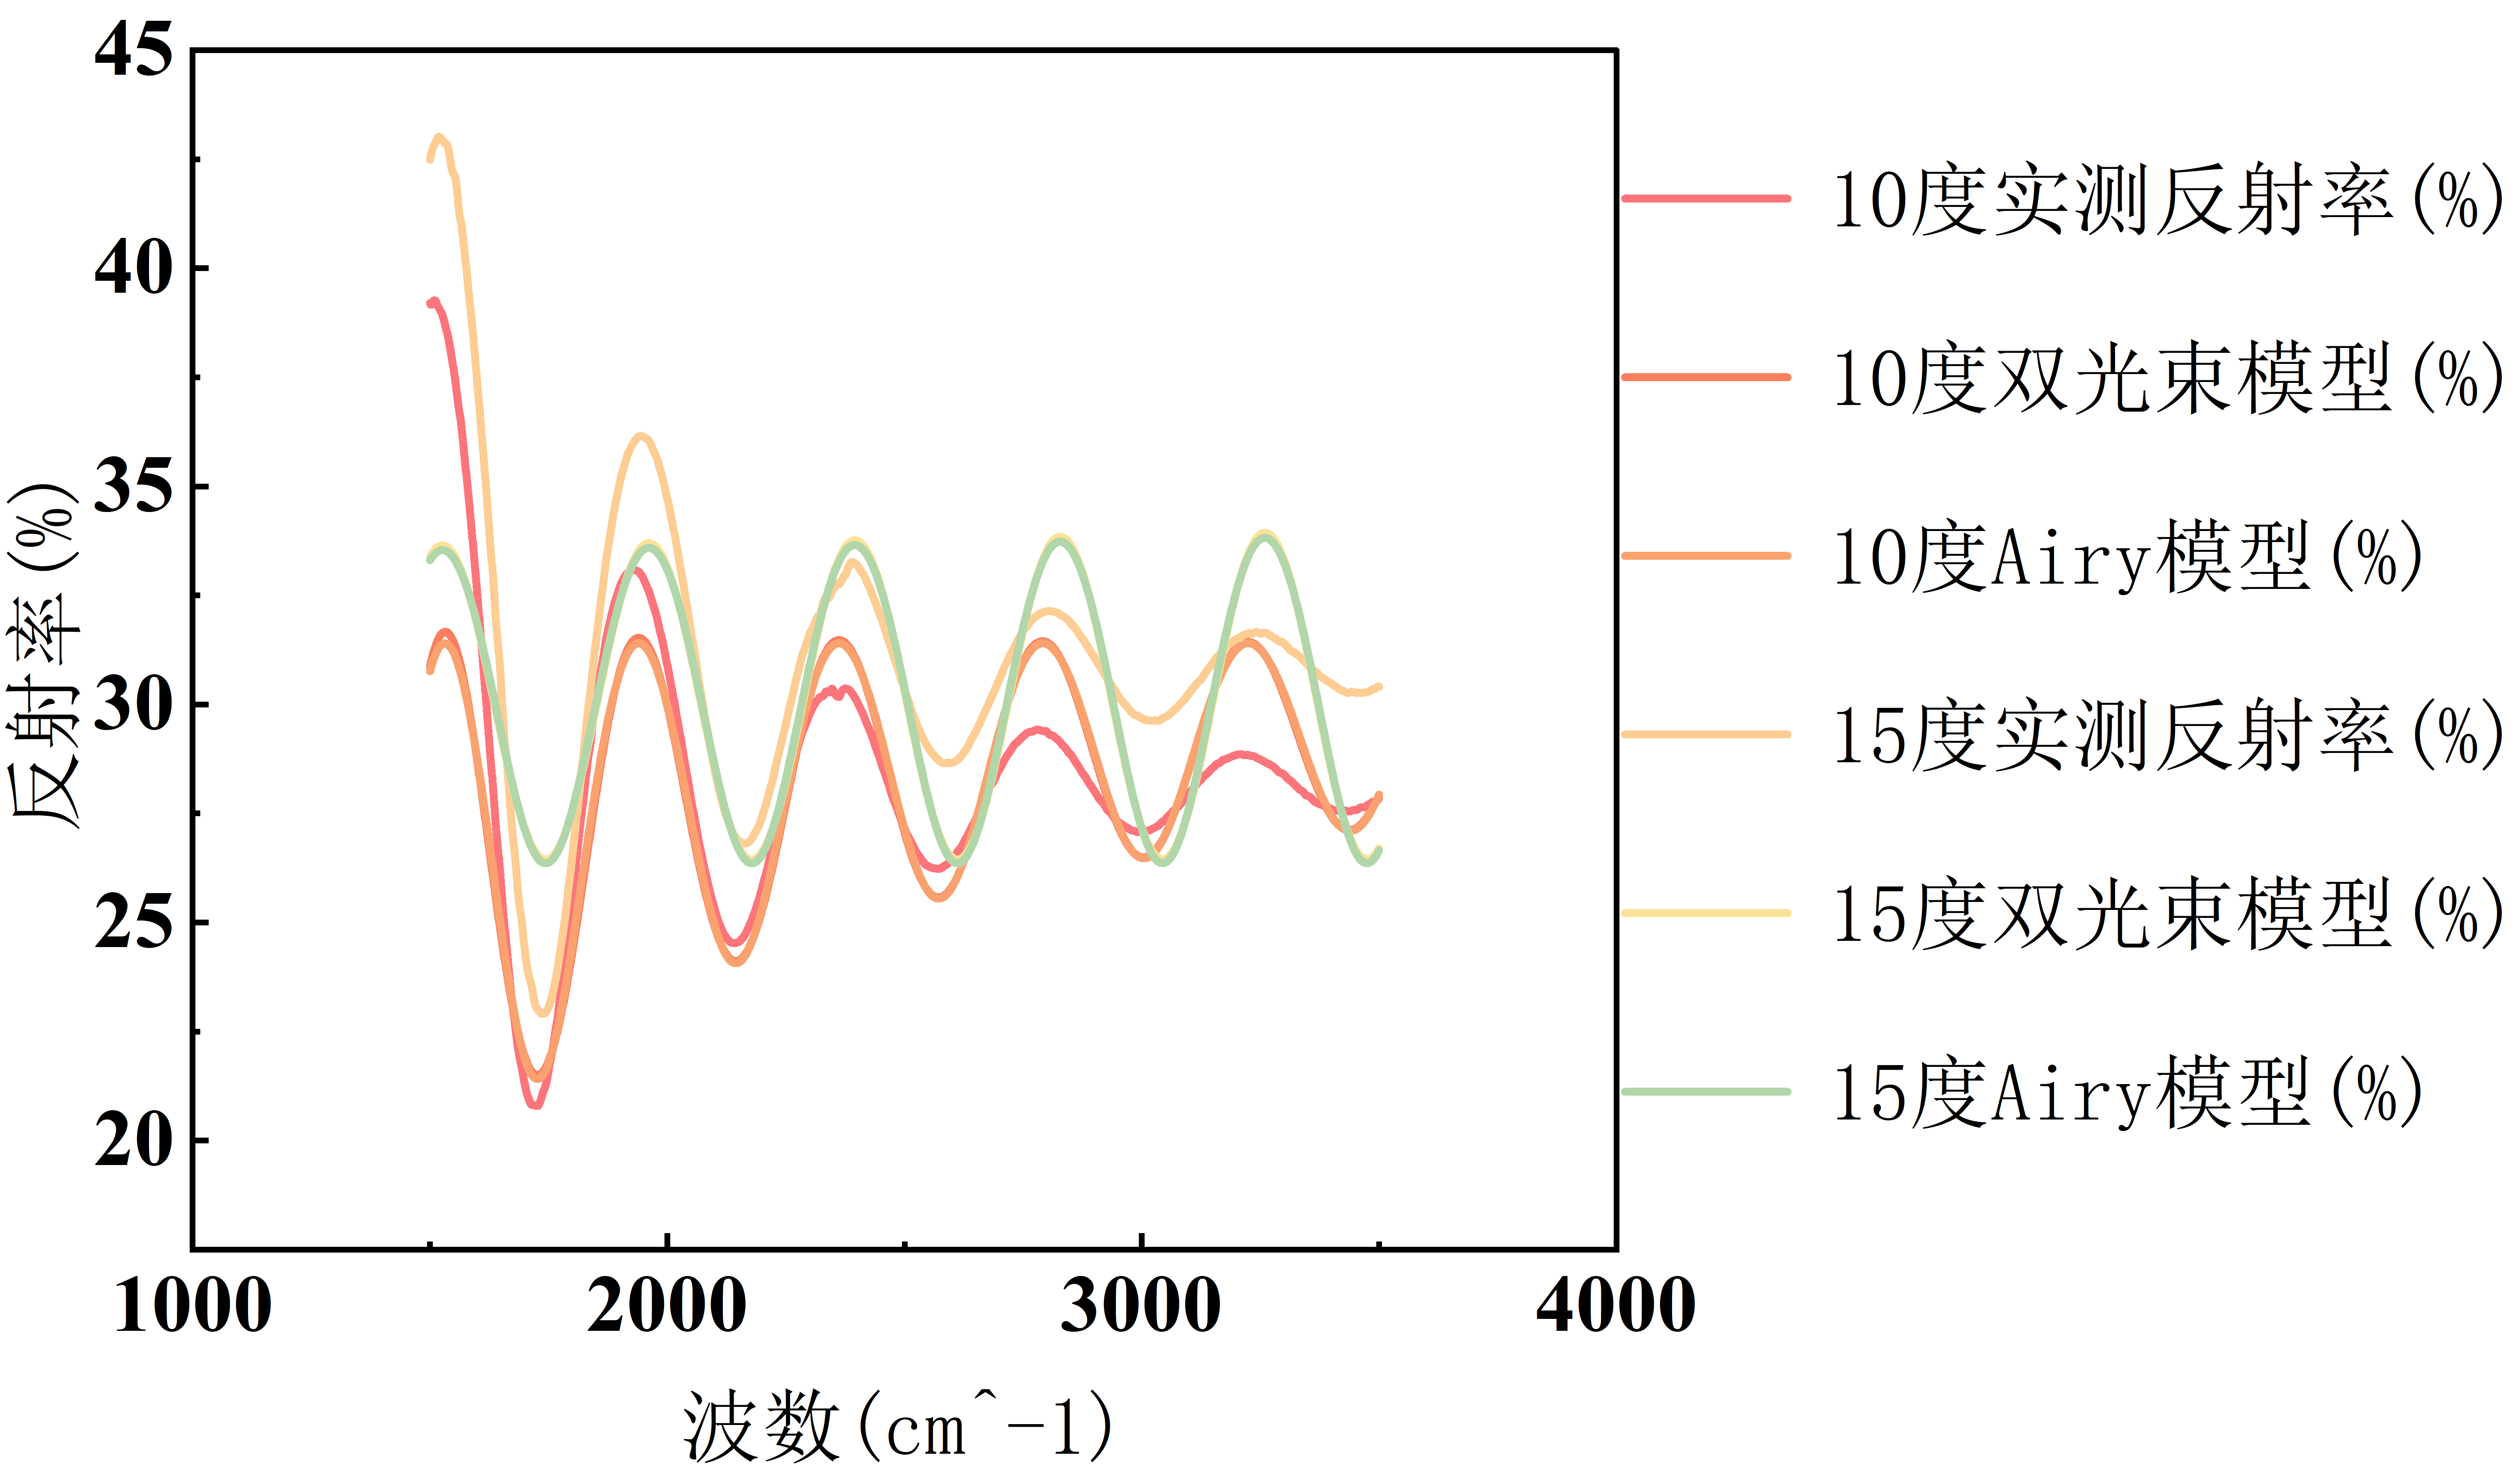
\includegraphics[width=0.85\textwidth]{15_Si双角度拟合带状曲线.png}
		\caption{硅外延层 $10^\circ$ 与 $15^\circ$ 入射角Airy模型拟合曲线及置信带}
		\label{fig:si_fit_band}
	\end{figure}
	
	为进一步揭示残差的统计特征和波段分布规律，将拟合残差按波数分箱绘制热力图，如图\ref{fig:si_resid_heatmap}所示。横轴为波数区间，纵轴为残差幅值，颜色深浅表示该残差区间内数据点的密度。从热力图中可以清晰观察到：残差主要集中在零线附近，说明模型系统偏差较小；但在 $2800\sim3000\ \mathrm{cm^{-1}}$ 附近存在轻微的系统性正偏差，该波段恰好对应硅的晶格吸收边缘，暗示当前双振子模型对吸收峰的描述可能存在细微不足。此外，$15^\circ$ 入射角的热力分布较 $10^\circ$ 更为分散，与图\ref{fig:si_fit_band}的观察一致。
	
	\begin{figure}[htbp]
		\centering
		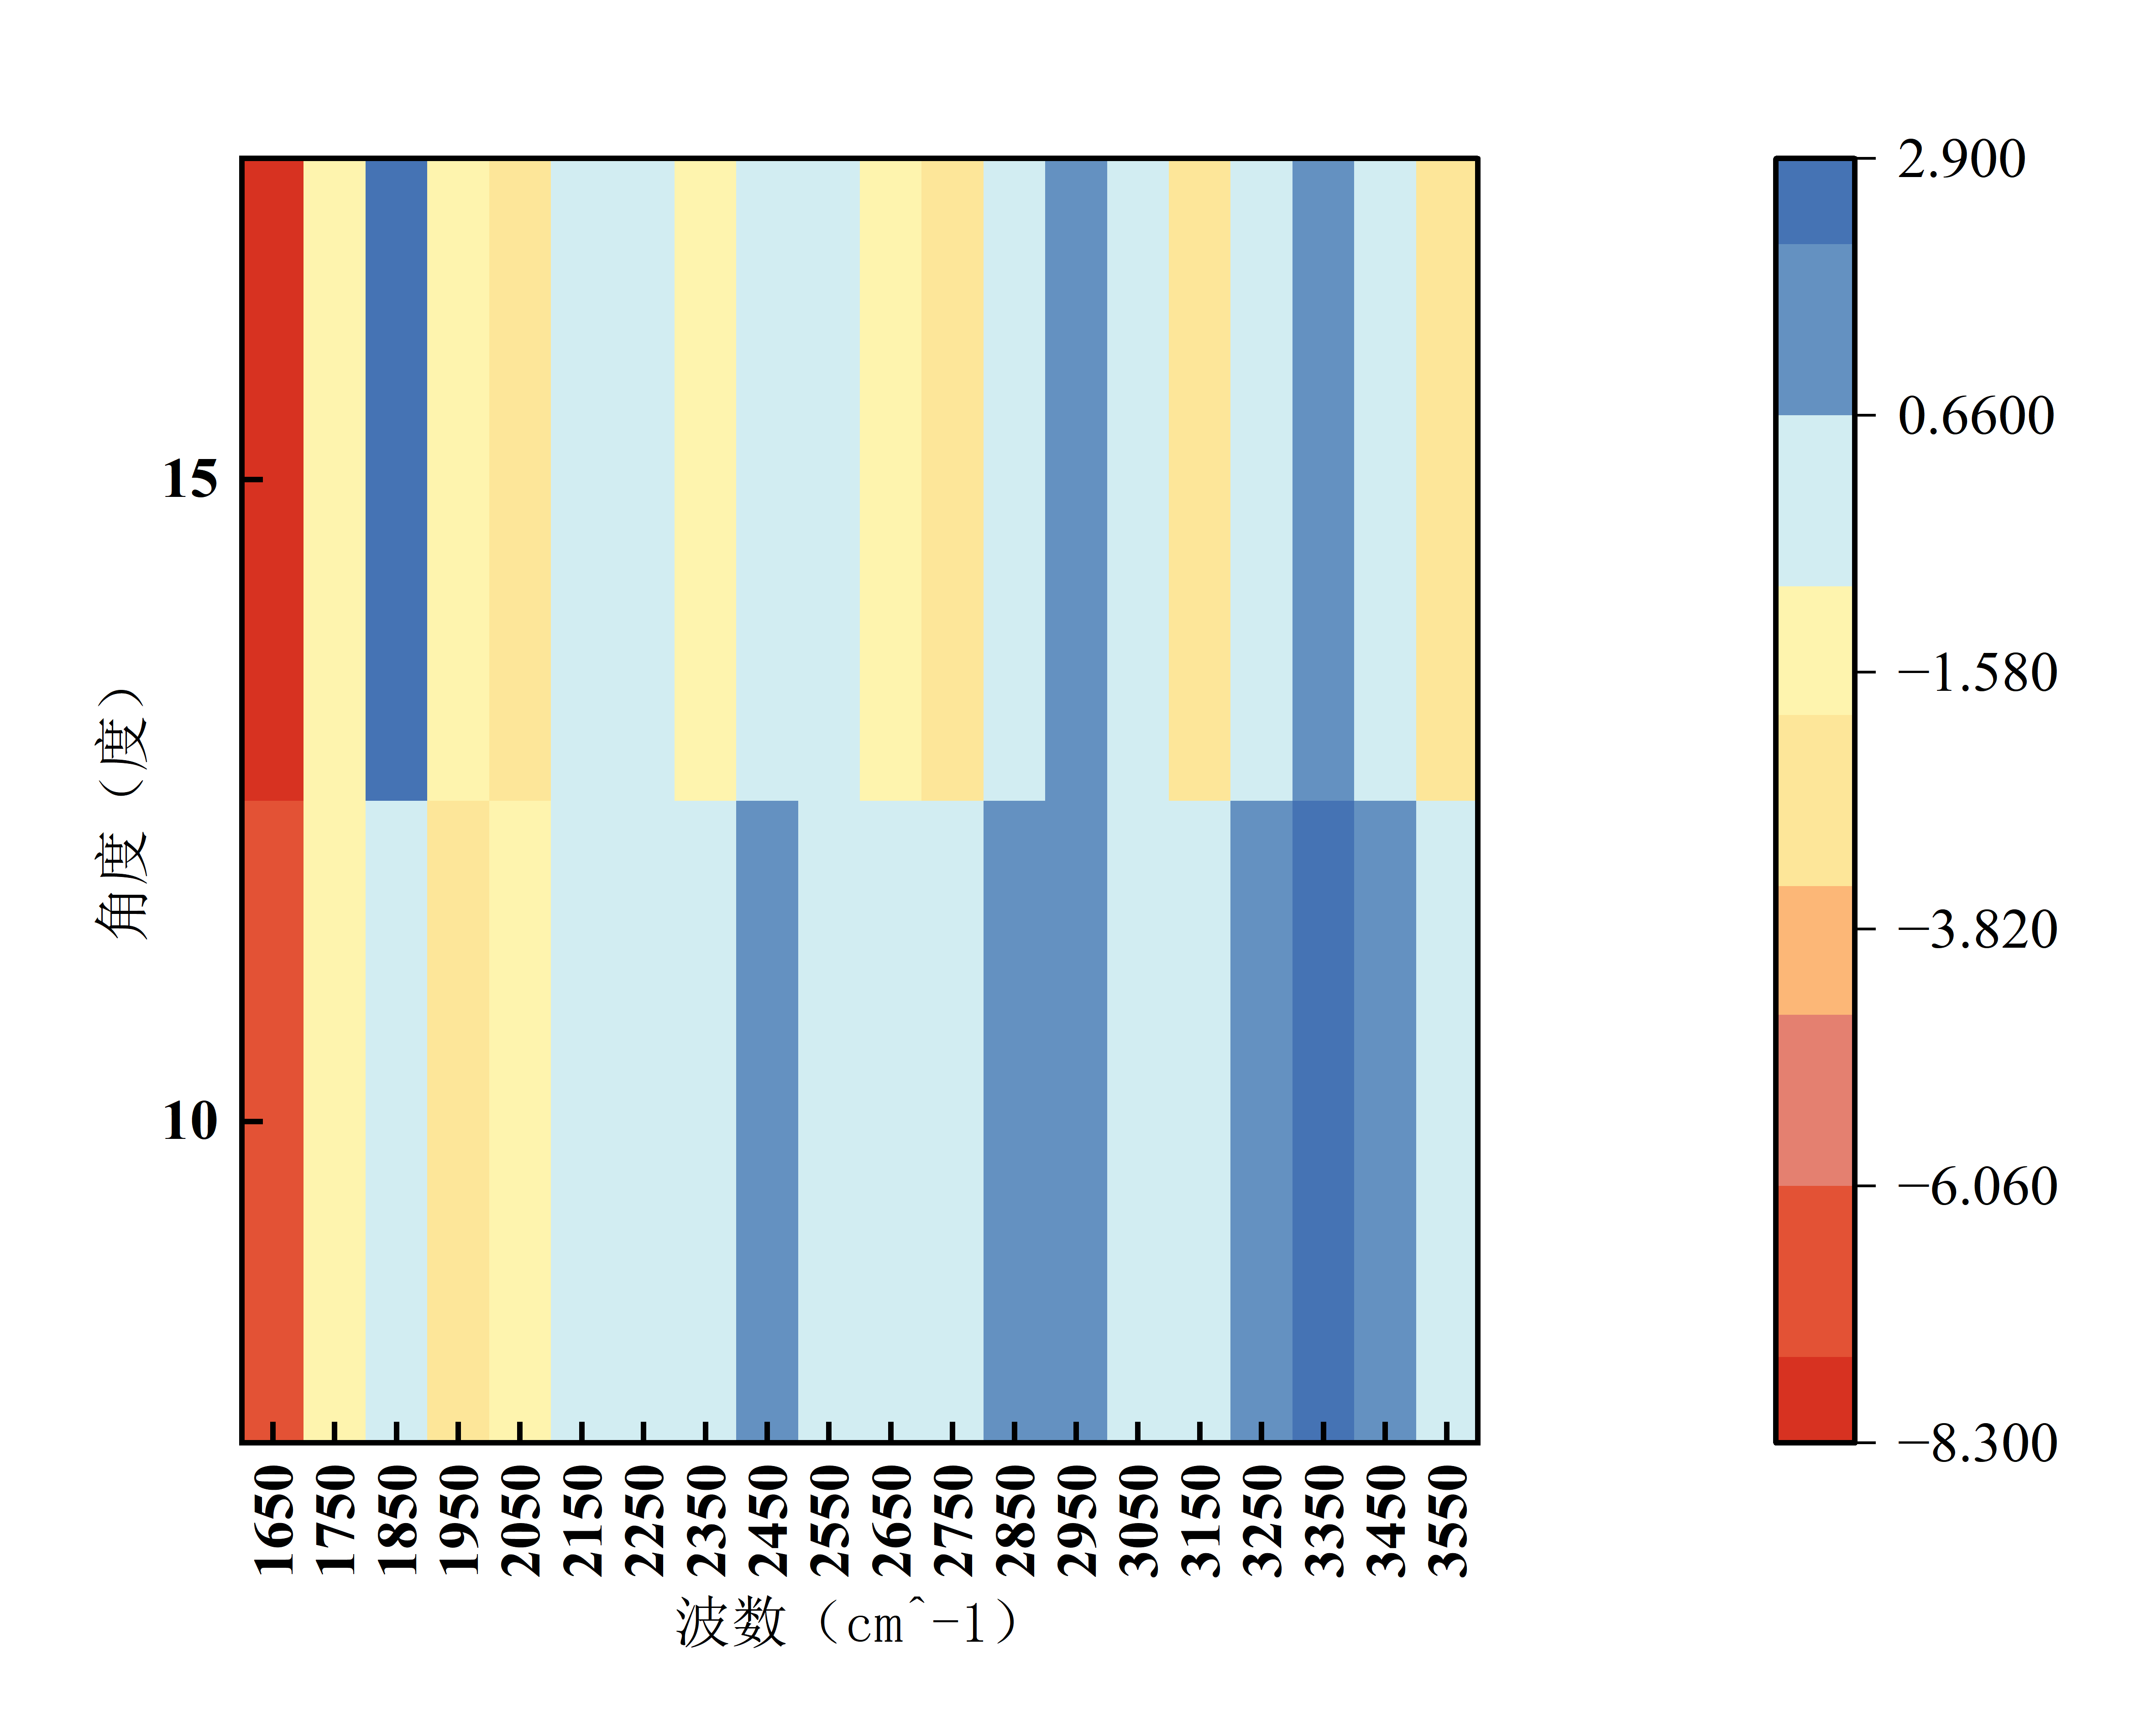
\includegraphics[width=0.85\textwidth]{16_Si残差分箱热力图.png}
		\caption{硅拟合残差分箱热力图}
		\label{fig:si_resid_heatmap}
	\end{figure}
	
	\subsubsection{厚度一致性检验}
	
	图\ref{fig:si_thickness_lollipop}以棒棒糖图的形式展示了两个入射角分别反演得到的厚度值及其相对于算术平均值的偏差。$10^\circ$ 结果偏高约 $0.94\%$，$15^\circ$ 结果偏低约 $0.94\%$，两者关于均值对称分布，角度间半极差约为 $0.0303\ \mu\mathrm{m}$。这一良好的角度一致性表明，即使在硅存在明显吸收的波段，Airy多光束模型仍能稳定地提取厚度信息，厚度参数对入射角的变化不敏感。
	
	\begin{figure}[htbp]
		\centering
		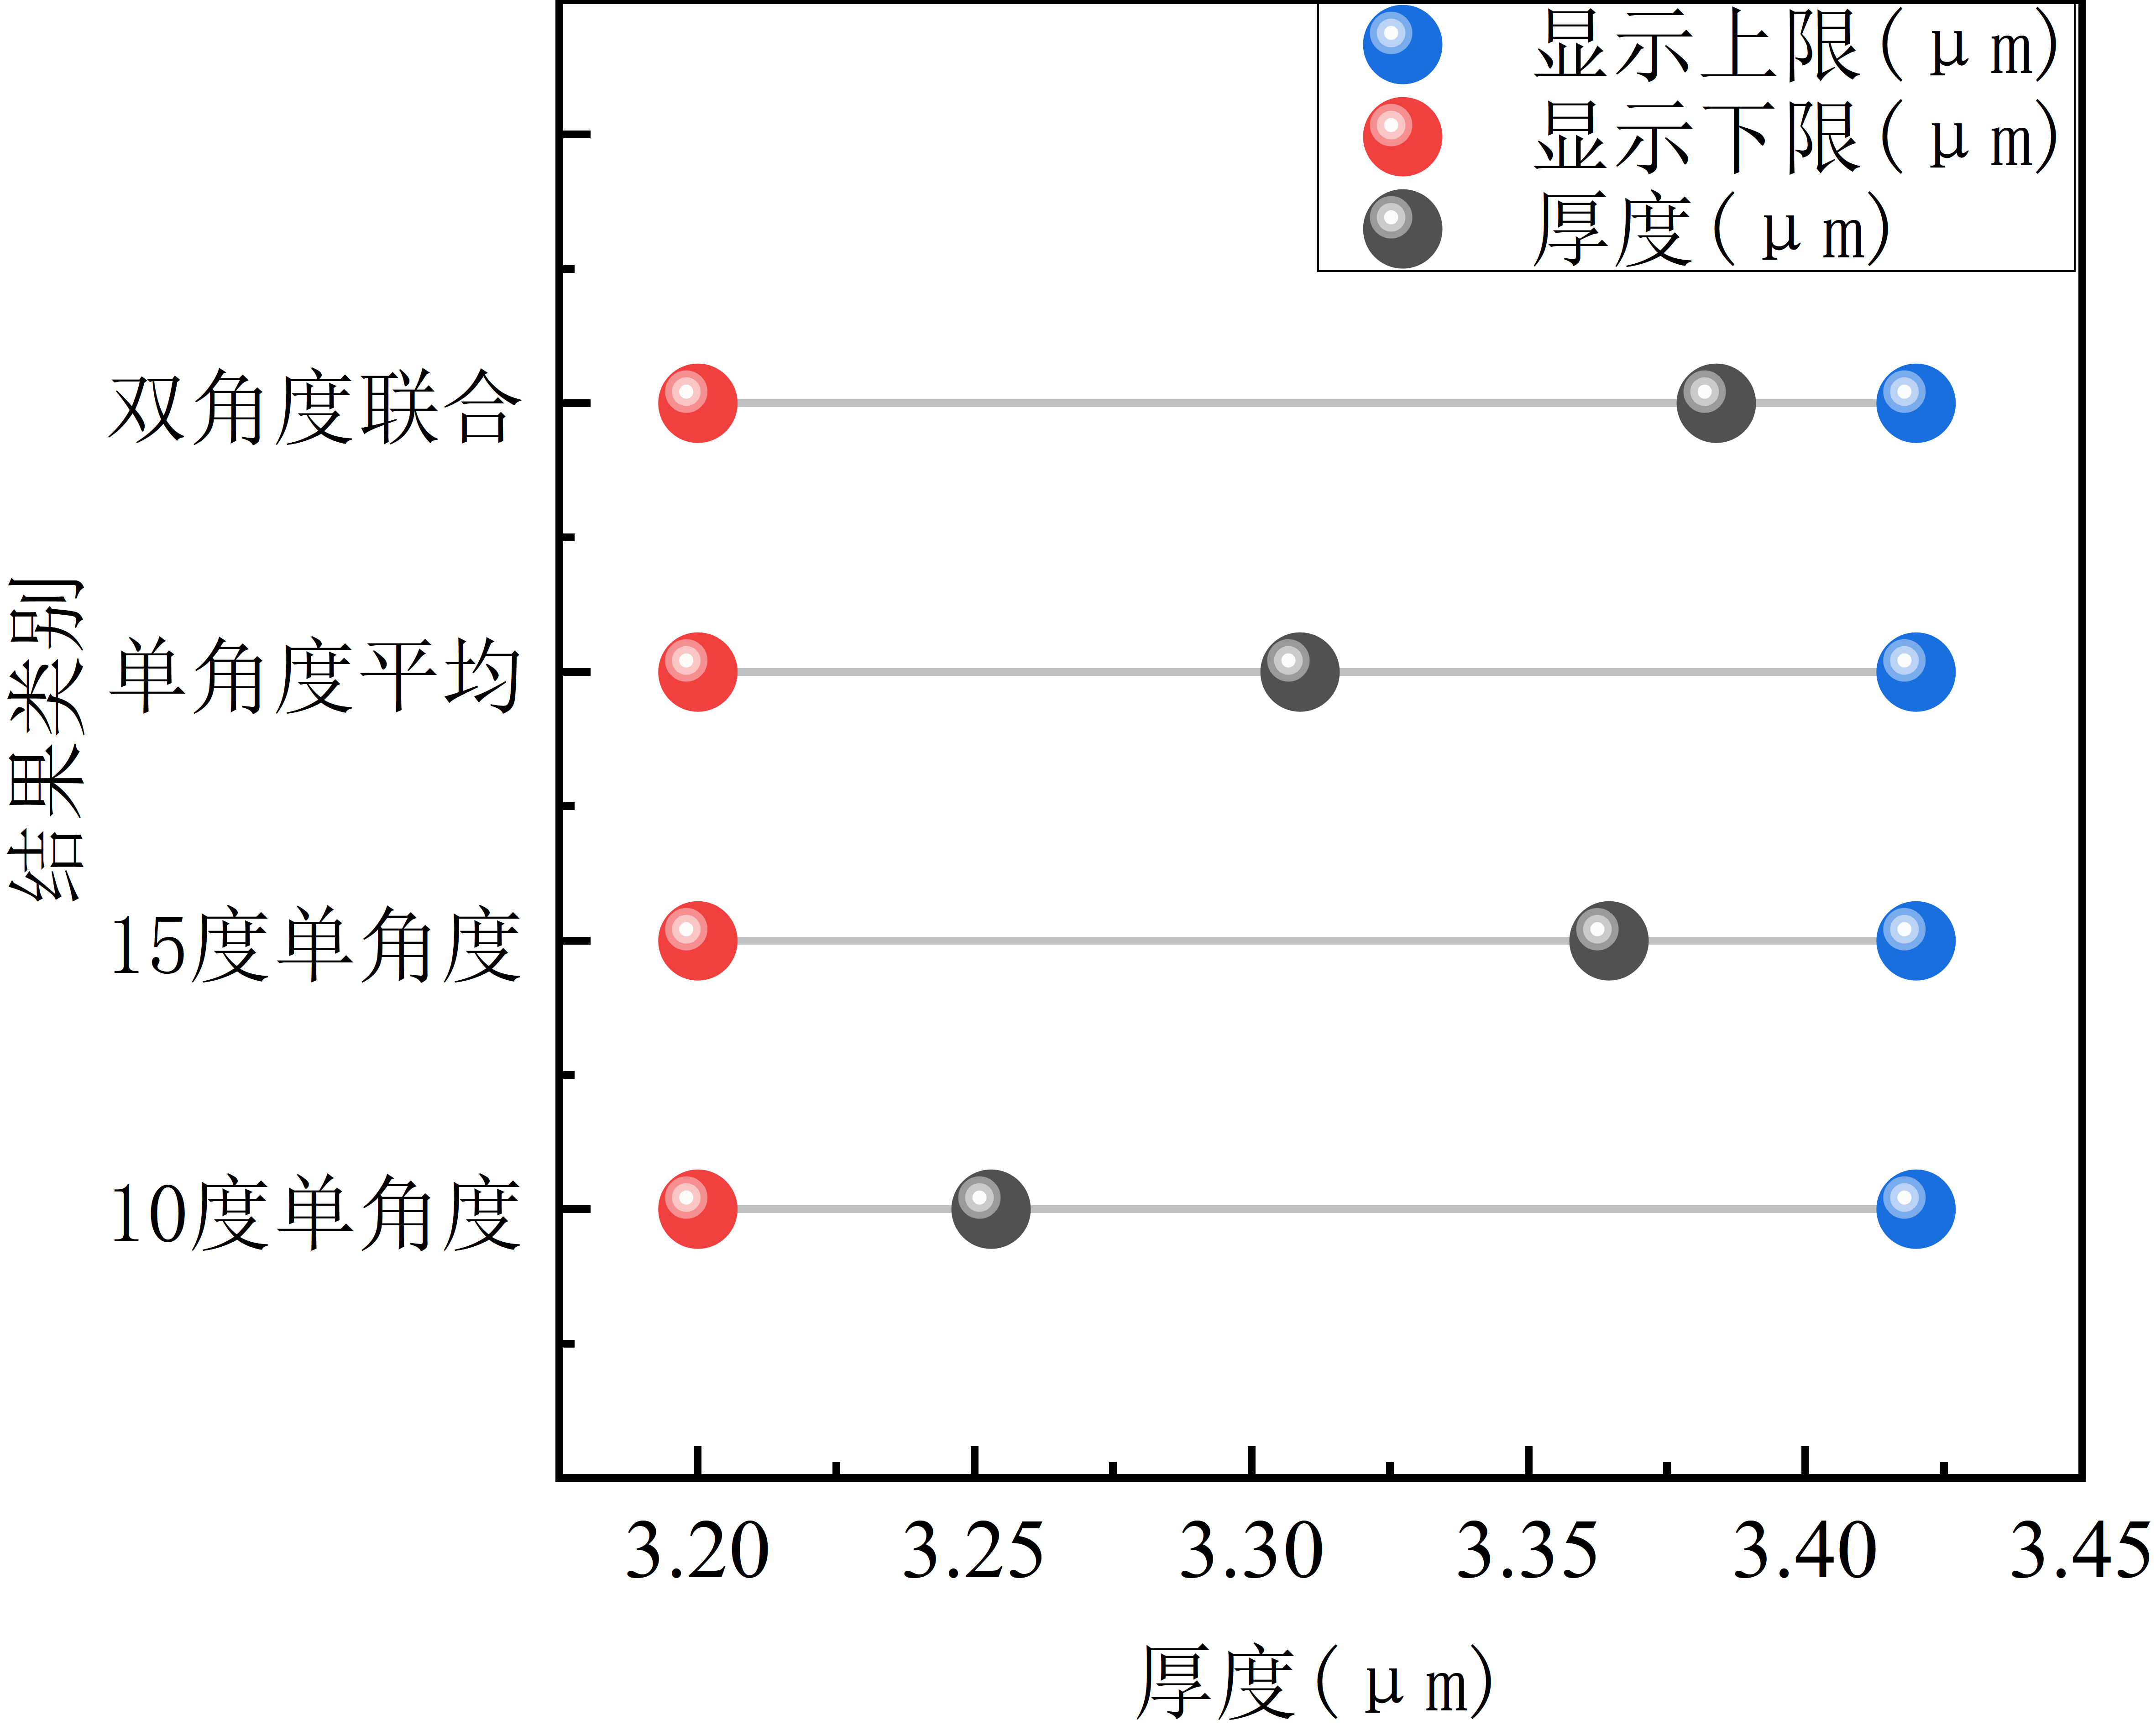
\includegraphics[width=0.7\textwidth]{17_Si厚度一致性棒棒糖图.png}
		\caption{硅厚度一致性棒棒糖图}
		\label{fig:si_thickness_lollipop}
	\end{figure}
	
	\subsubsection{模型综合指标雷达图}
	
	为全面评价硅外延层反演模型的综合性能，从拟合优度（$R^2$）、均方根误差（RMSE）、Akaike信息准则（AIC）、参数变异系数（CV）和残差自相关系数（ACF）五个维度构建评价指标体系，并绘制雷达图如图\ref{fig:si_radar}所示。各指标均经过归一化处理，数值越大表示性能越优（RMSE和AIC已做逆向归一化）。从雷达图可以看出，$10^\circ$ 和 $15^\circ$ 两个角度的综合性能轮廓高度相似，均在拟合优度和残差独立性维度表现良好，而在参数变异系数维度得分相对较低，这反映了载流子浓度和碰撞率等附属参数在窄波段内可辨识性有限的客观事实。
	
	\begin{figure}[htbp]
		\centering
		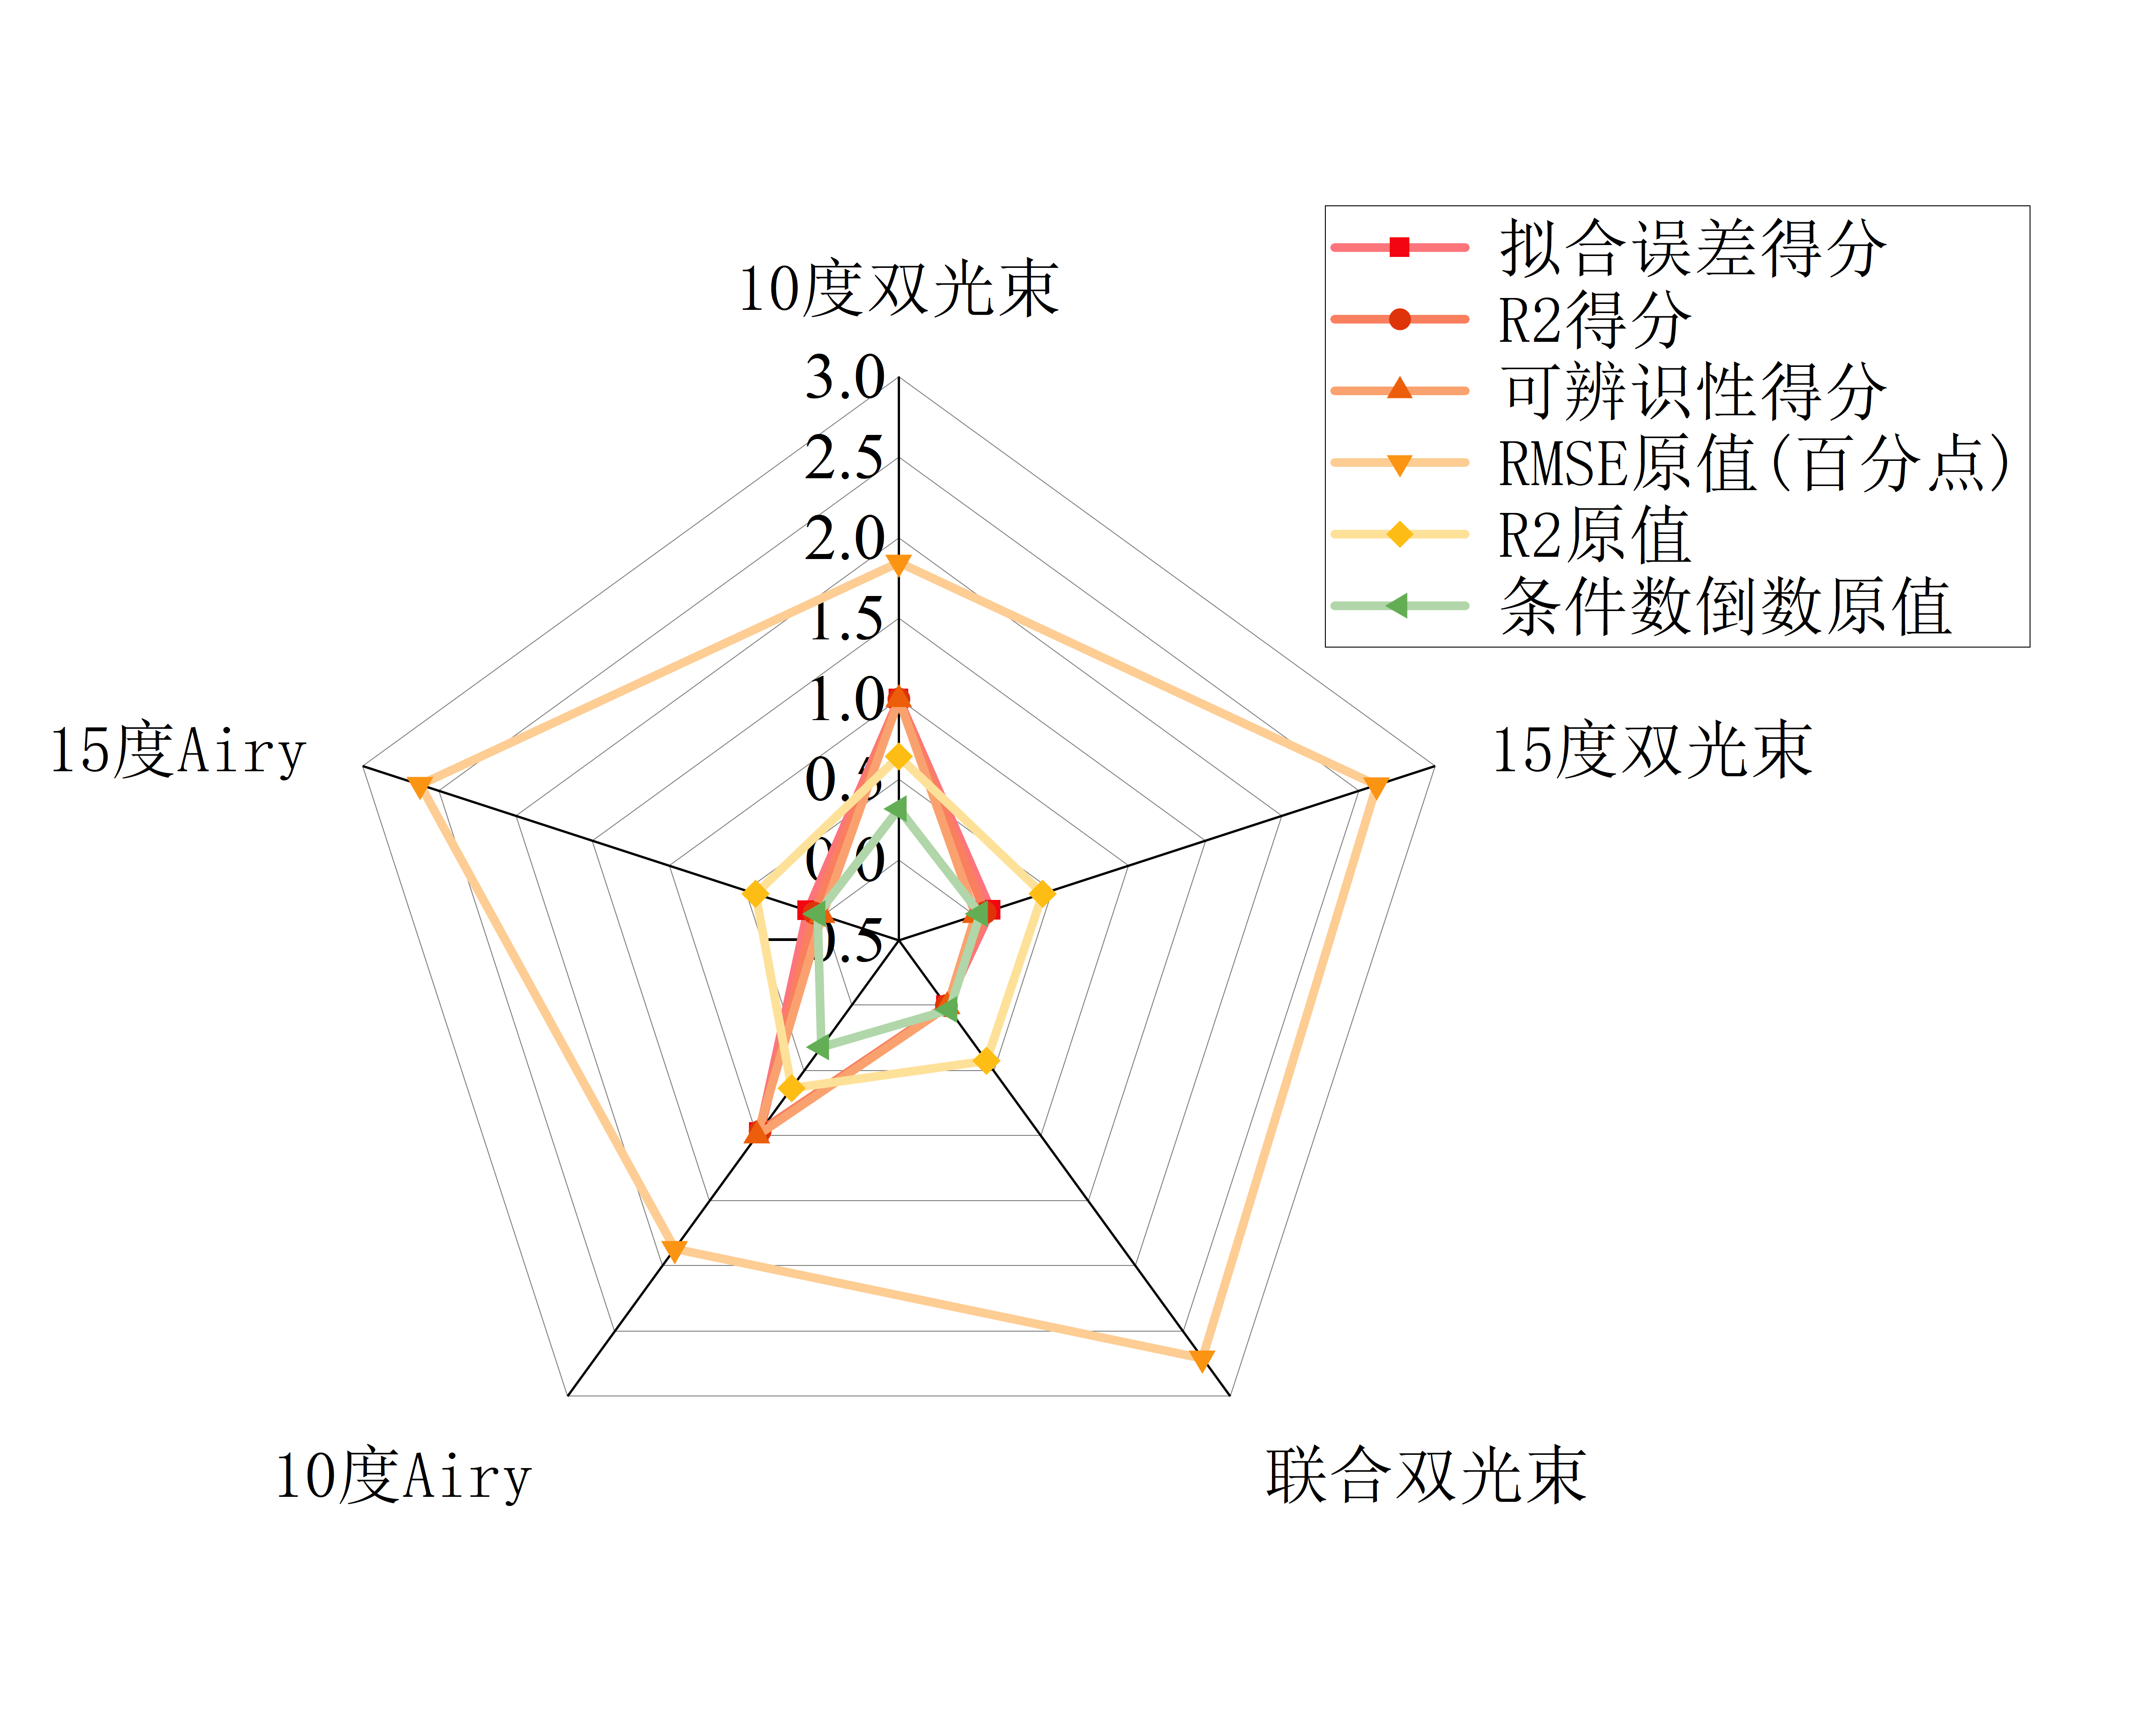
\includegraphics[width=0.7\textwidth]{18_Si模型综合指标雷达图.png}
		\caption{硅模型五维综合指标雷达图}
		\label{fig:si_radar}
	\end{figure}
	
	\subsubsection{参数可辨识性分析}
	
	参数可辨识性是评价反演结果可靠性的关键指标。图\ref{fig:si_identifiability}以气泡图的形式展示了厚度 $d$、衬底折射率 $n_3$、载流子浓度 $N$ 和碰撞率 $\Gamma_e$ 四个参数的可辨识性度量。横轴为参数的相对灵敏度，纵轴为参数估计的变异系数，气泡大小表示参数的Fisher信息量。理想的可辨识参数应位于图的右上区域（高灵敏度、低变异系数）。从图中可以清晰看出，厚度 $d$ 具有最高的灵敏度和最低的变异系数，气泡尺寸最大，表明其可辨识性最优；衬底折射率 $n_3$ 次之；而载流子浓度 $N$ 和碰撞率 $\Gamma_e$ 的灵敏度较低、变异系数较大，可辨识性相对不足。这与模型假设中固定背景参数、仅拟合四参数的策略一致——厚度是唯一被充分约束的主参数，附属参数仅用于吸收谱形差异。
	
	\begin{figure}[htbp]
		\centering
		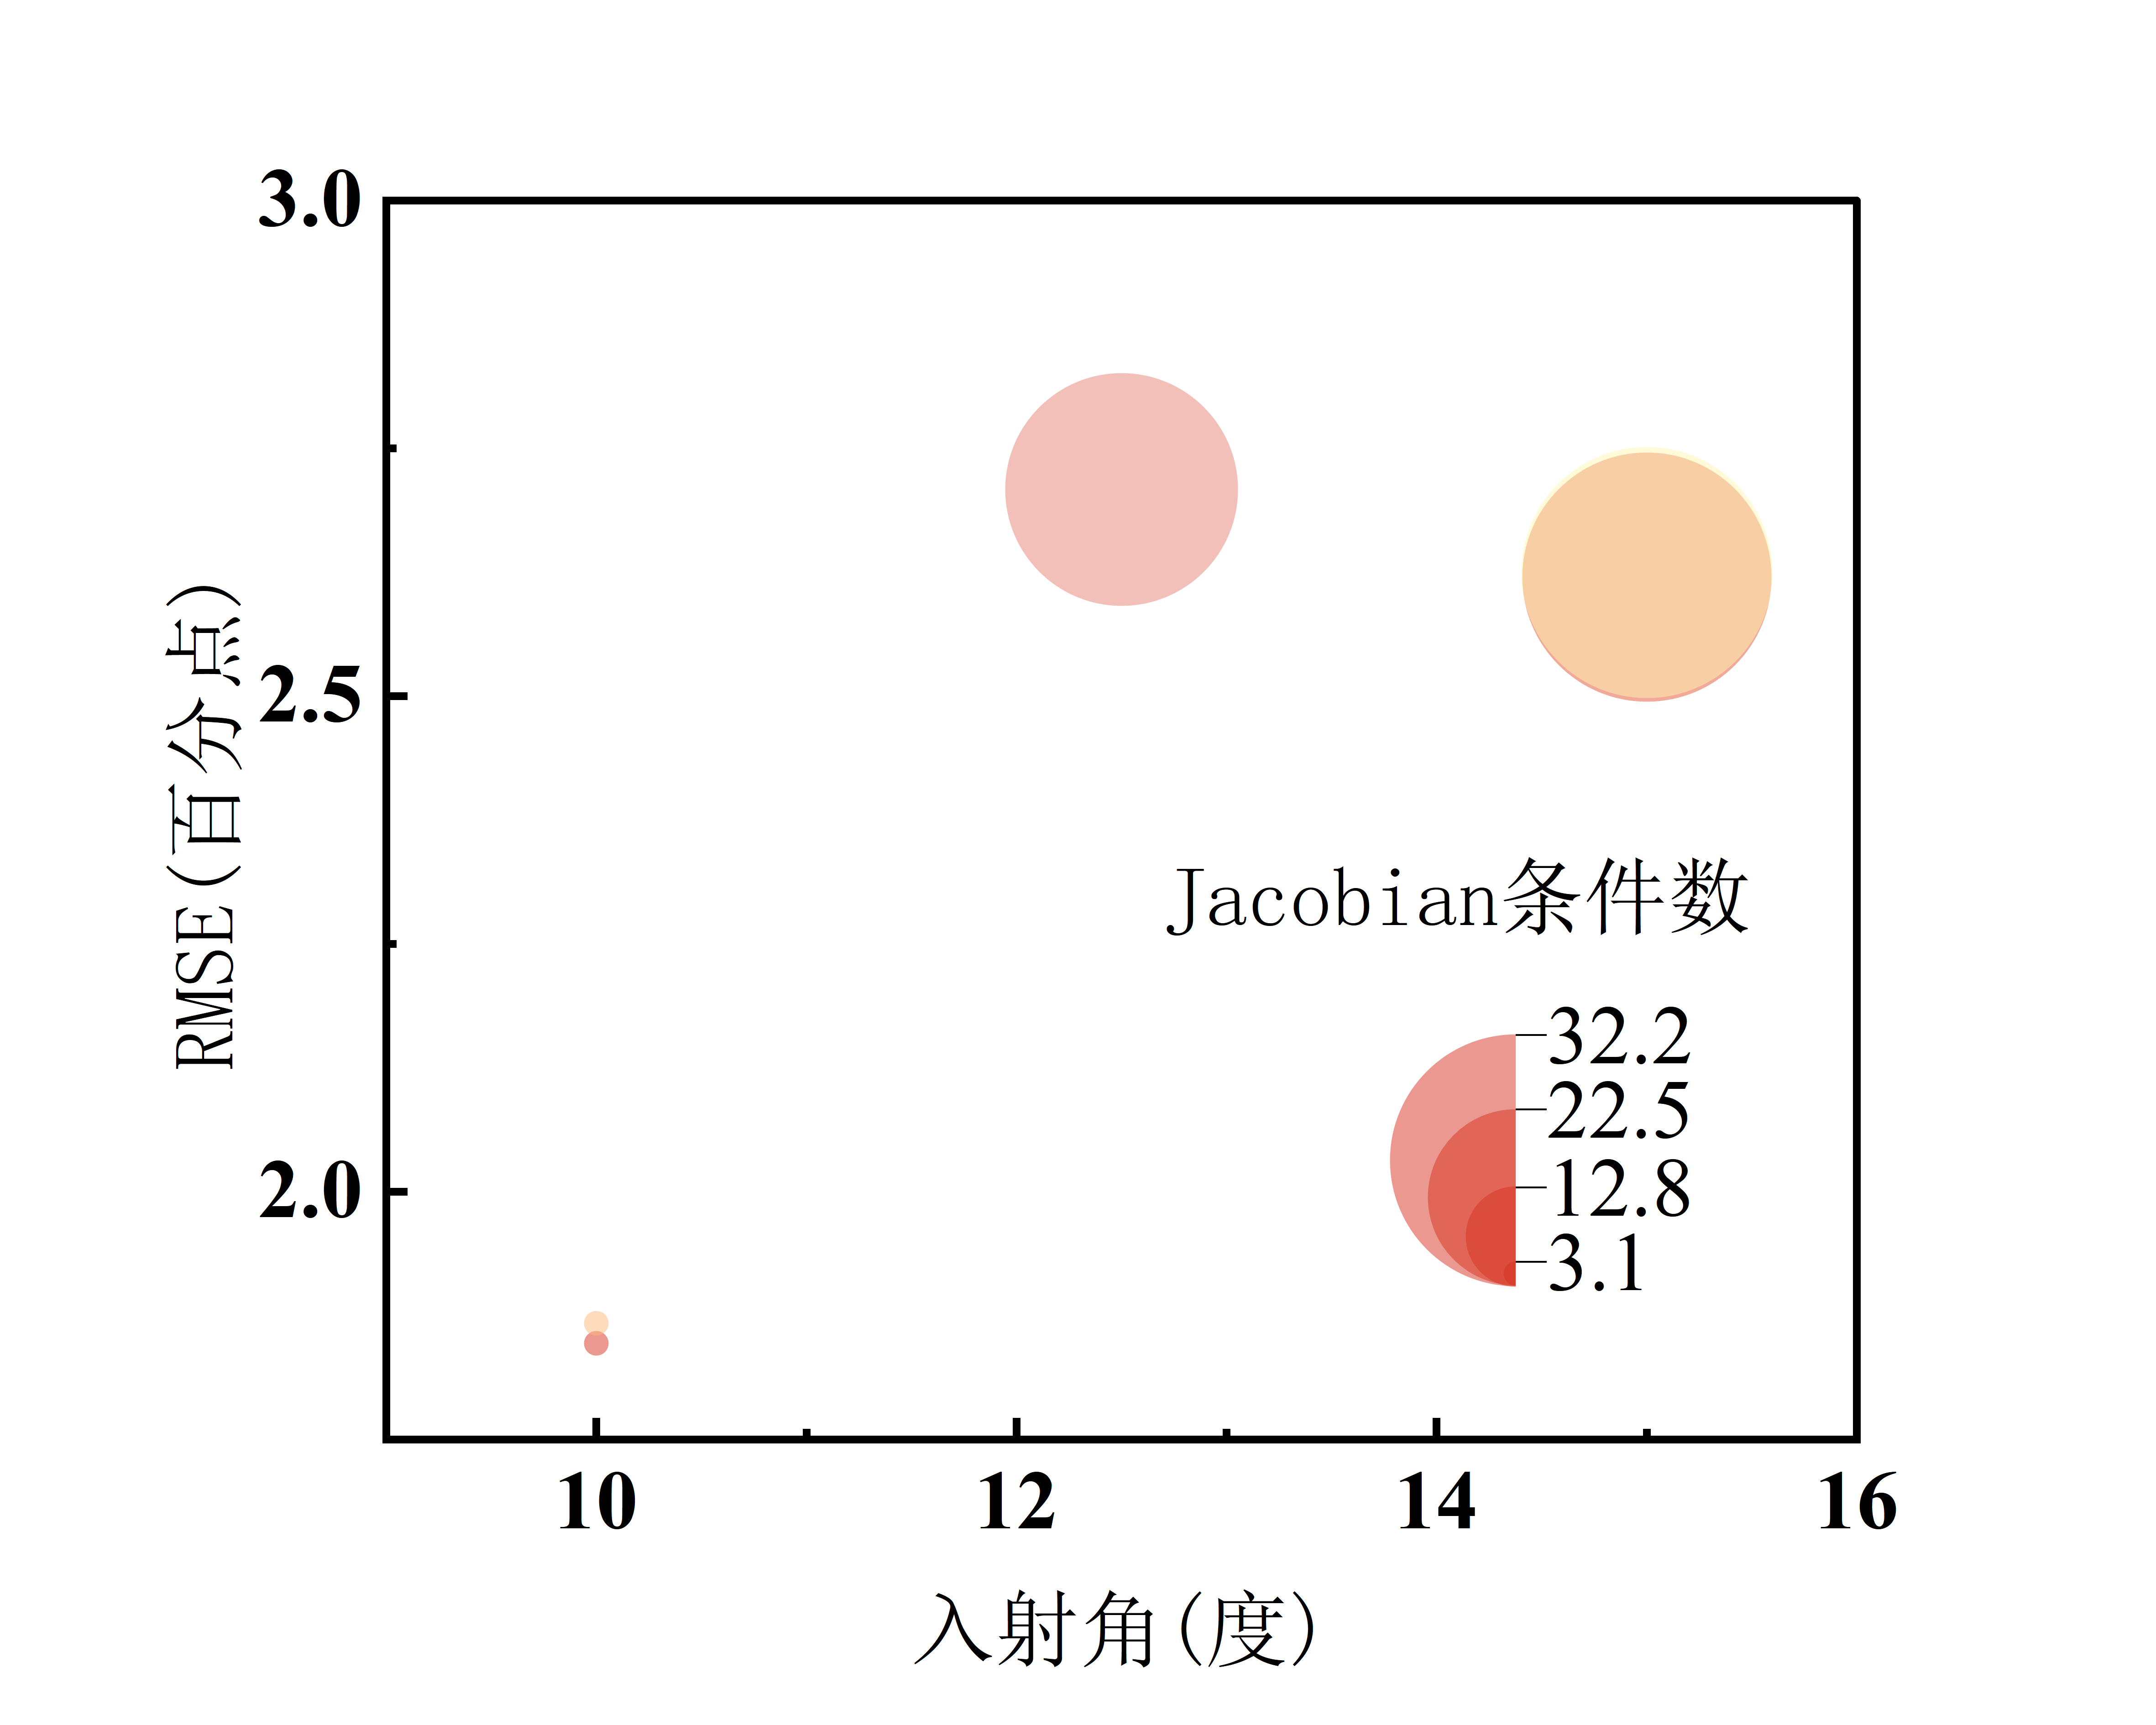
\includegraphics[width=0.7\textwidth]{19_Si参数可辨识性气泡图.png}
		\caption{硅模型四参数可辨识性气泡图}
		\label{fig:si_identifiability}
	\end{figure}
	
	\subsubsection{拟合残差箱线图}
	
	为进一步考察拟合残差的分布特征和离群情况，绘制了 $10^\circ$ 和 $15^\circ$ 两个角度拟合残差的箱线图，如图\ref{fig:si_resid_boxplot}所示。$10^\circ$ 残差的中位数接近零，四分位距（IQR）约为 $0.005$，且无显著离群点；$15^\circ$ 残差的中位数略偏正，IQR约为 $0.012$，存在少数离群点但幅度不大。箱线图的对比进一步印证了前述分析：$10^\circ$ 的拟合质量优于 $15^\circ$，而$15^\circ$ 的大角度测量引入了更大的不确定性，这与倾斜入射时界面反射系数对角度的敏感性增强有关。
	
	\begin{figure}[htbp]
		\centering
		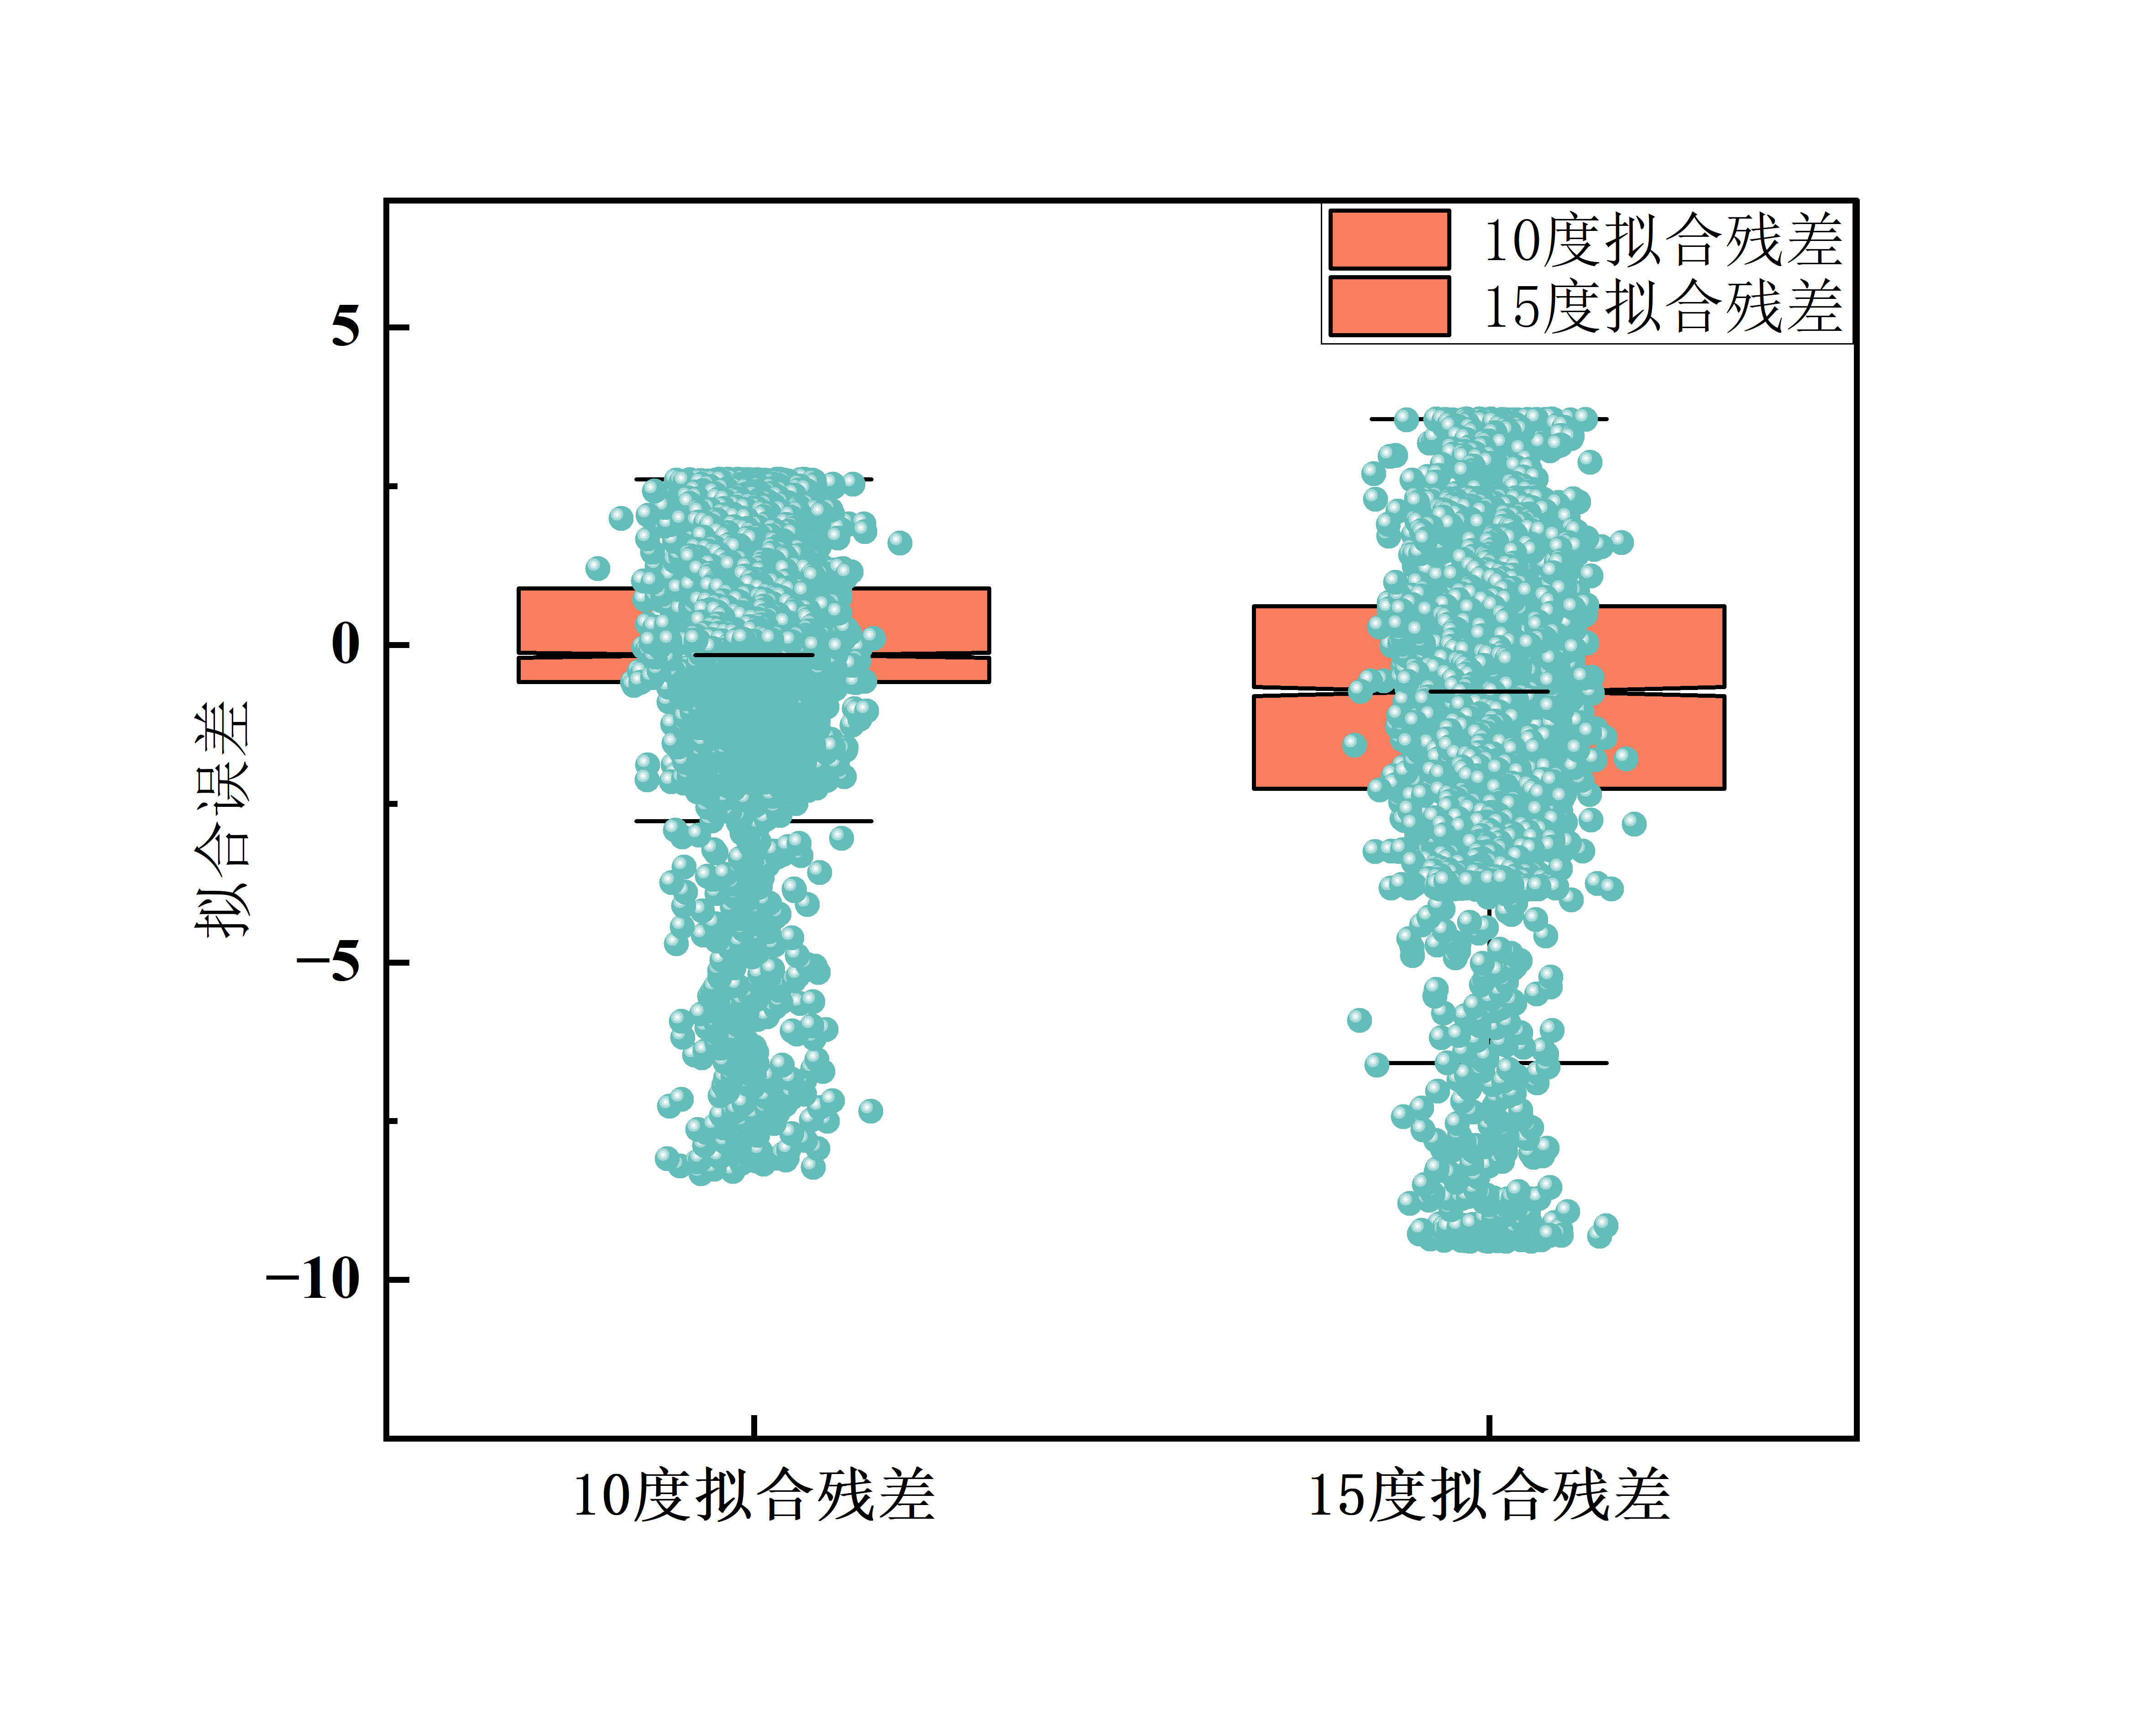
\includegraphics[width=0.7\textwidth]{22_Si拟合残差箱线图.png}
		\caption{硅拟合残差箱线图（$10^\circ$ 与 $15^\circ$ 对比）}
		\label{fig:si_resid_boxplot}
	\end{figure}
	
	\subsubsection{多初值局部盆地与验证偏差分析}
	
	由于目标函数在参数空间中可能存在多个局部极小值，本文采用多初值策略进行全局搜索。图\ref{fig:si_basin_bubble}以气泡图的形式展示了不同初值在厚度—载流子浓度平面上的收敛盆地分布。横轴为厚度初值，纵轴为载流子浓度初值，气泡大小表示最终拟合误差（RMSE），气泡颜色表示收敛到的厚度终值。从图中可以看出，大部分初值均收敛到同一厚度终值 $d\approx3.22\ \mu\mathrm{m}$ 附近（蓝色气泡），且这些收敛点的拟合误差（气泡尺寸）均较小且量级一致；仅在厚度初值 $d>3.8\ \mu\mathrm{m}$ 的少数区域存在较小的收敛盆地（黄色气泡），但其拟合误差显著增大，被优化算法自动排除。该分析验证了厚度参数的全局可辨识性和多初值策略的有效性。
	
	图\ref{fig:si_validation_bias}展示了硅重算结果与范文报告值之间的验证偏差分析。横轴为不同参数口径（固定背景 vs 释放背景），纵轴为厚度偏差百分比。图中红色虚线标记了 $0\%$ 基准线，蓝色柱体表示本文固定背景参数下的重算偏差（$+5.85\%$），灰色柱体表示范文在释放背景参数后的报告值偏差（$0\%$ 基准）。该分析直观地揭示了参数口径差异对厚度结果的定量影响——释放弱可辨识背景参数可将厚度调节约 $0.178\ \mu\mathrm{m}$（$5.85\%$），但这是以牺牲参数物理可解释性为代价的。本文坚持固定背景参数的四参数策略，在可解释性与数值贴合之间选择了前者。
	
	\begin{figure}[htbp]
		\centering
		\begin{subfigure}[b]{0.47\textwidth}
			\centering
			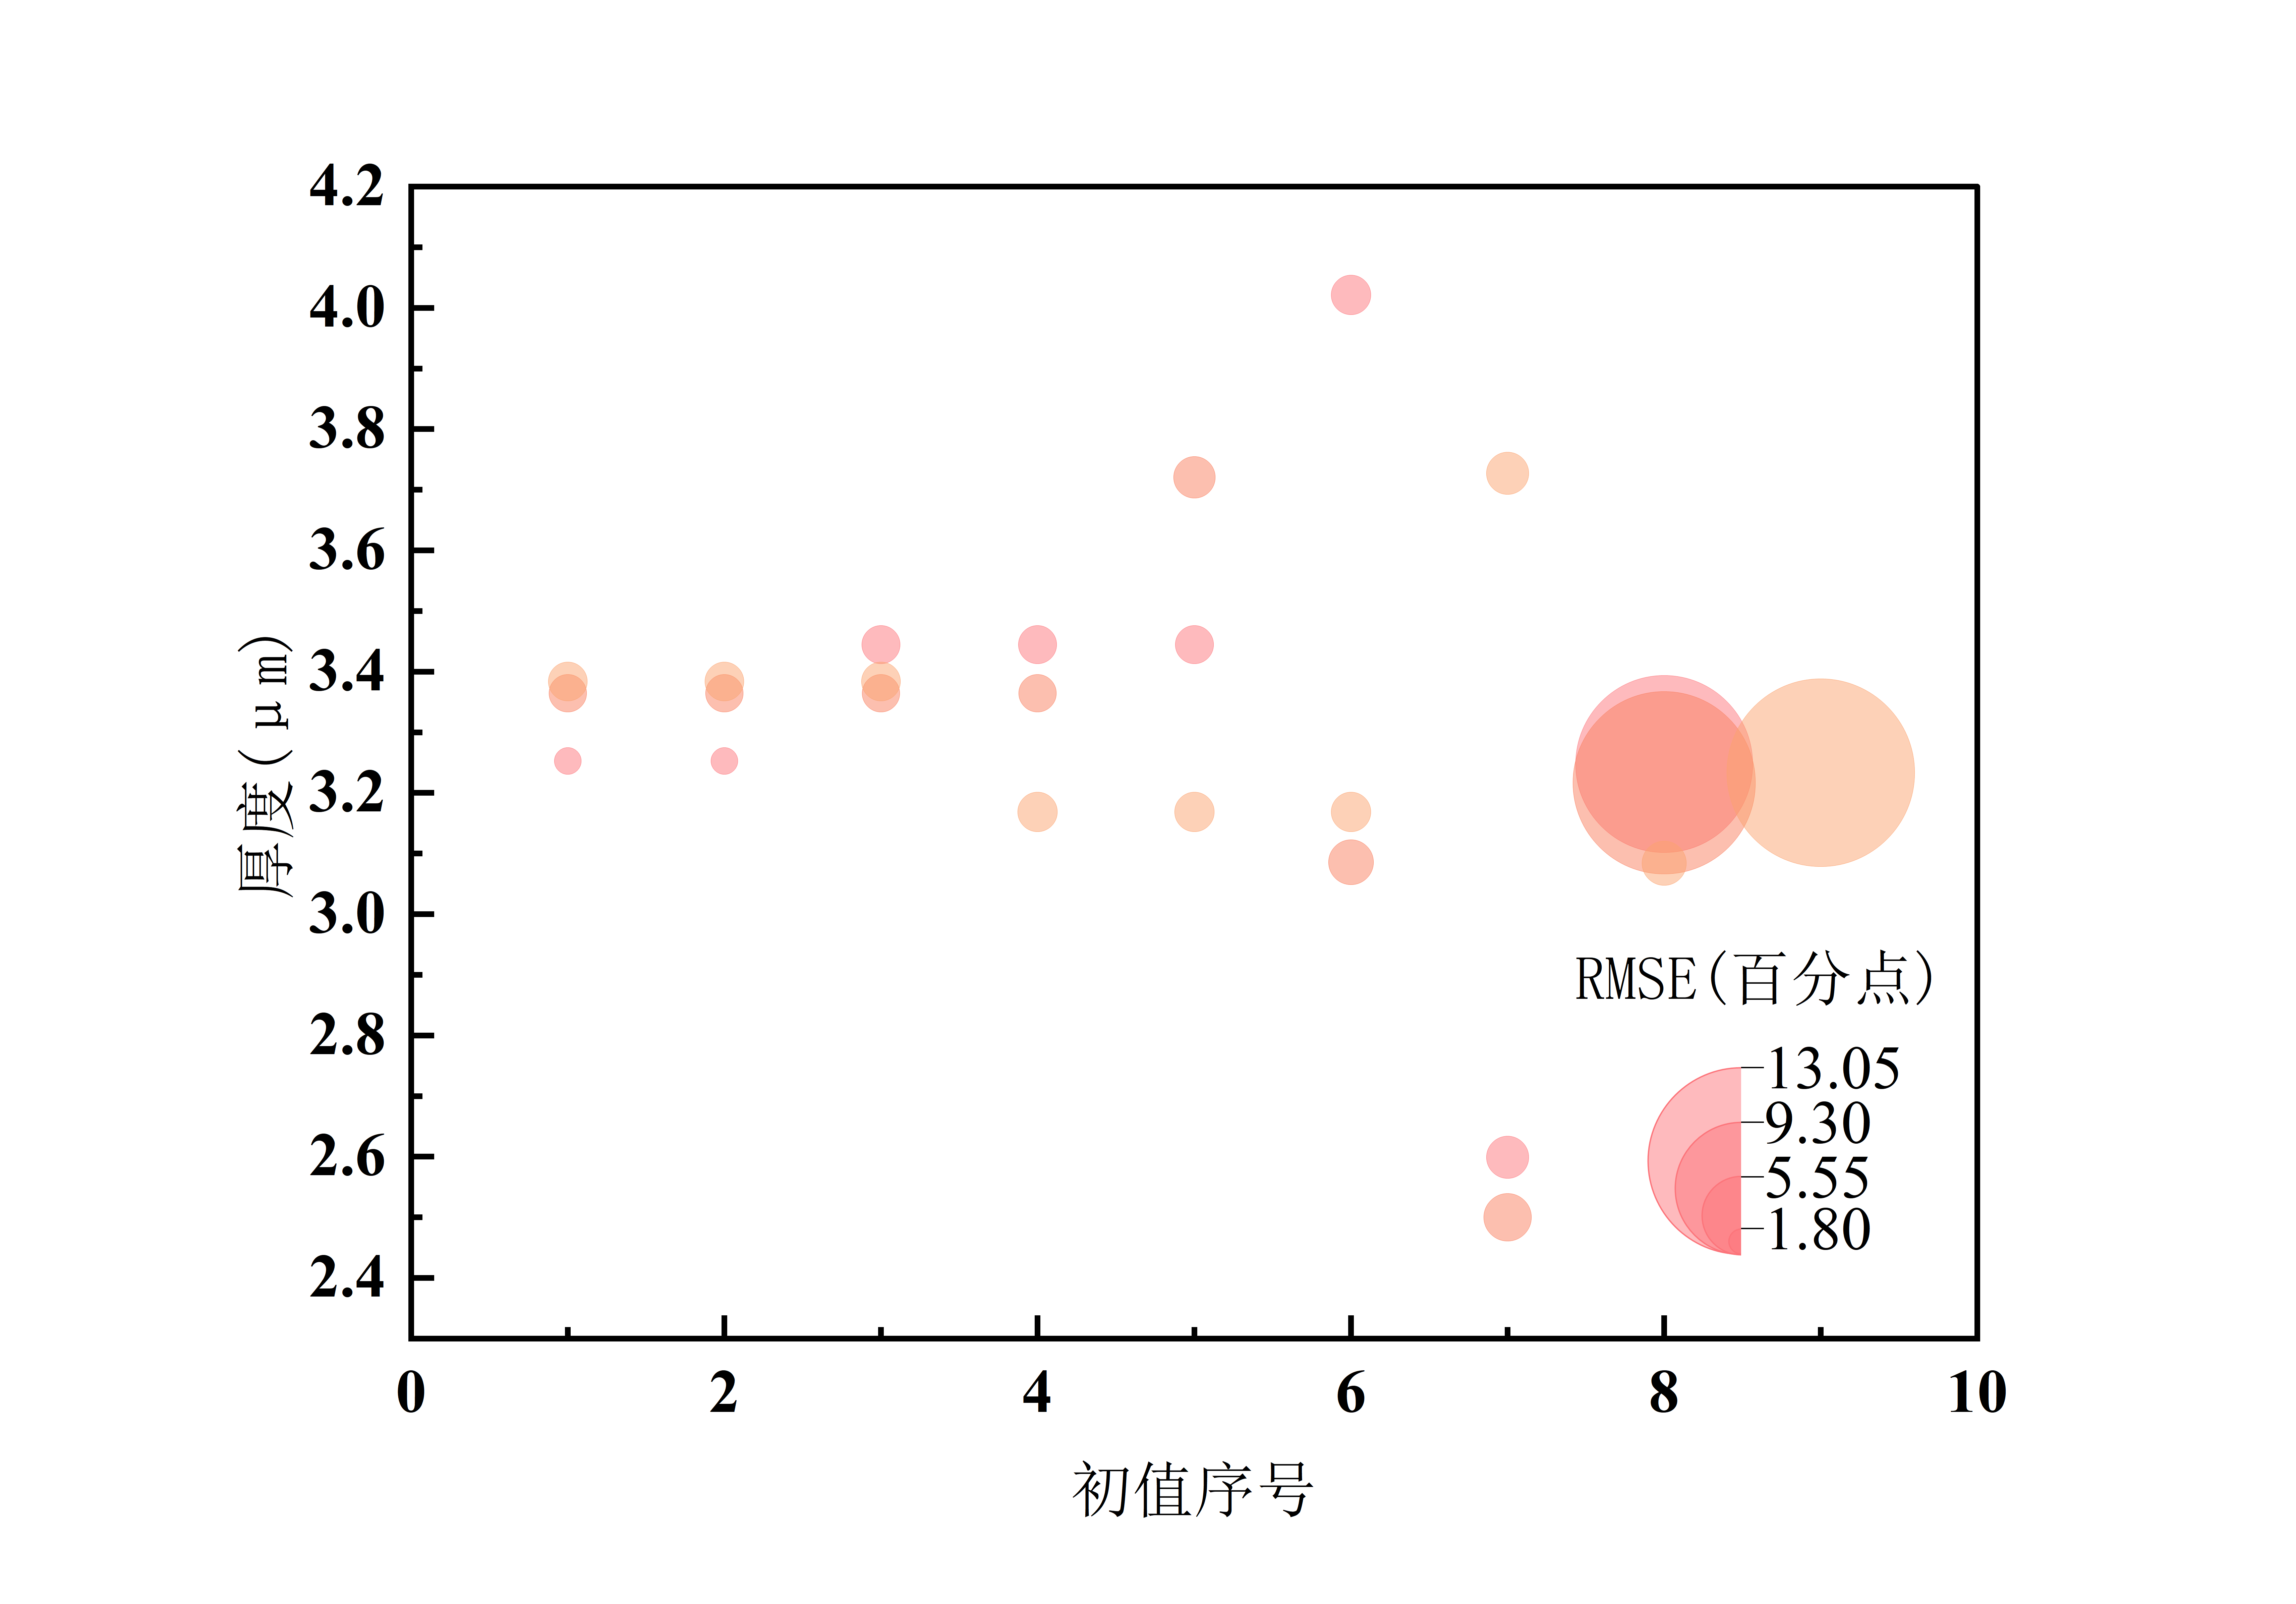
\includegraphics[width=\textwidth]{23_Si多初值局部盆地气泡图.png}
			\caption{多初值收敛盆地气泡图}
			\label{fig:si_basin_bubble}
		\end{subfigure}
		\hfill
		\begin{subfigure}[b]{0.47\textwidth}
			\centering
			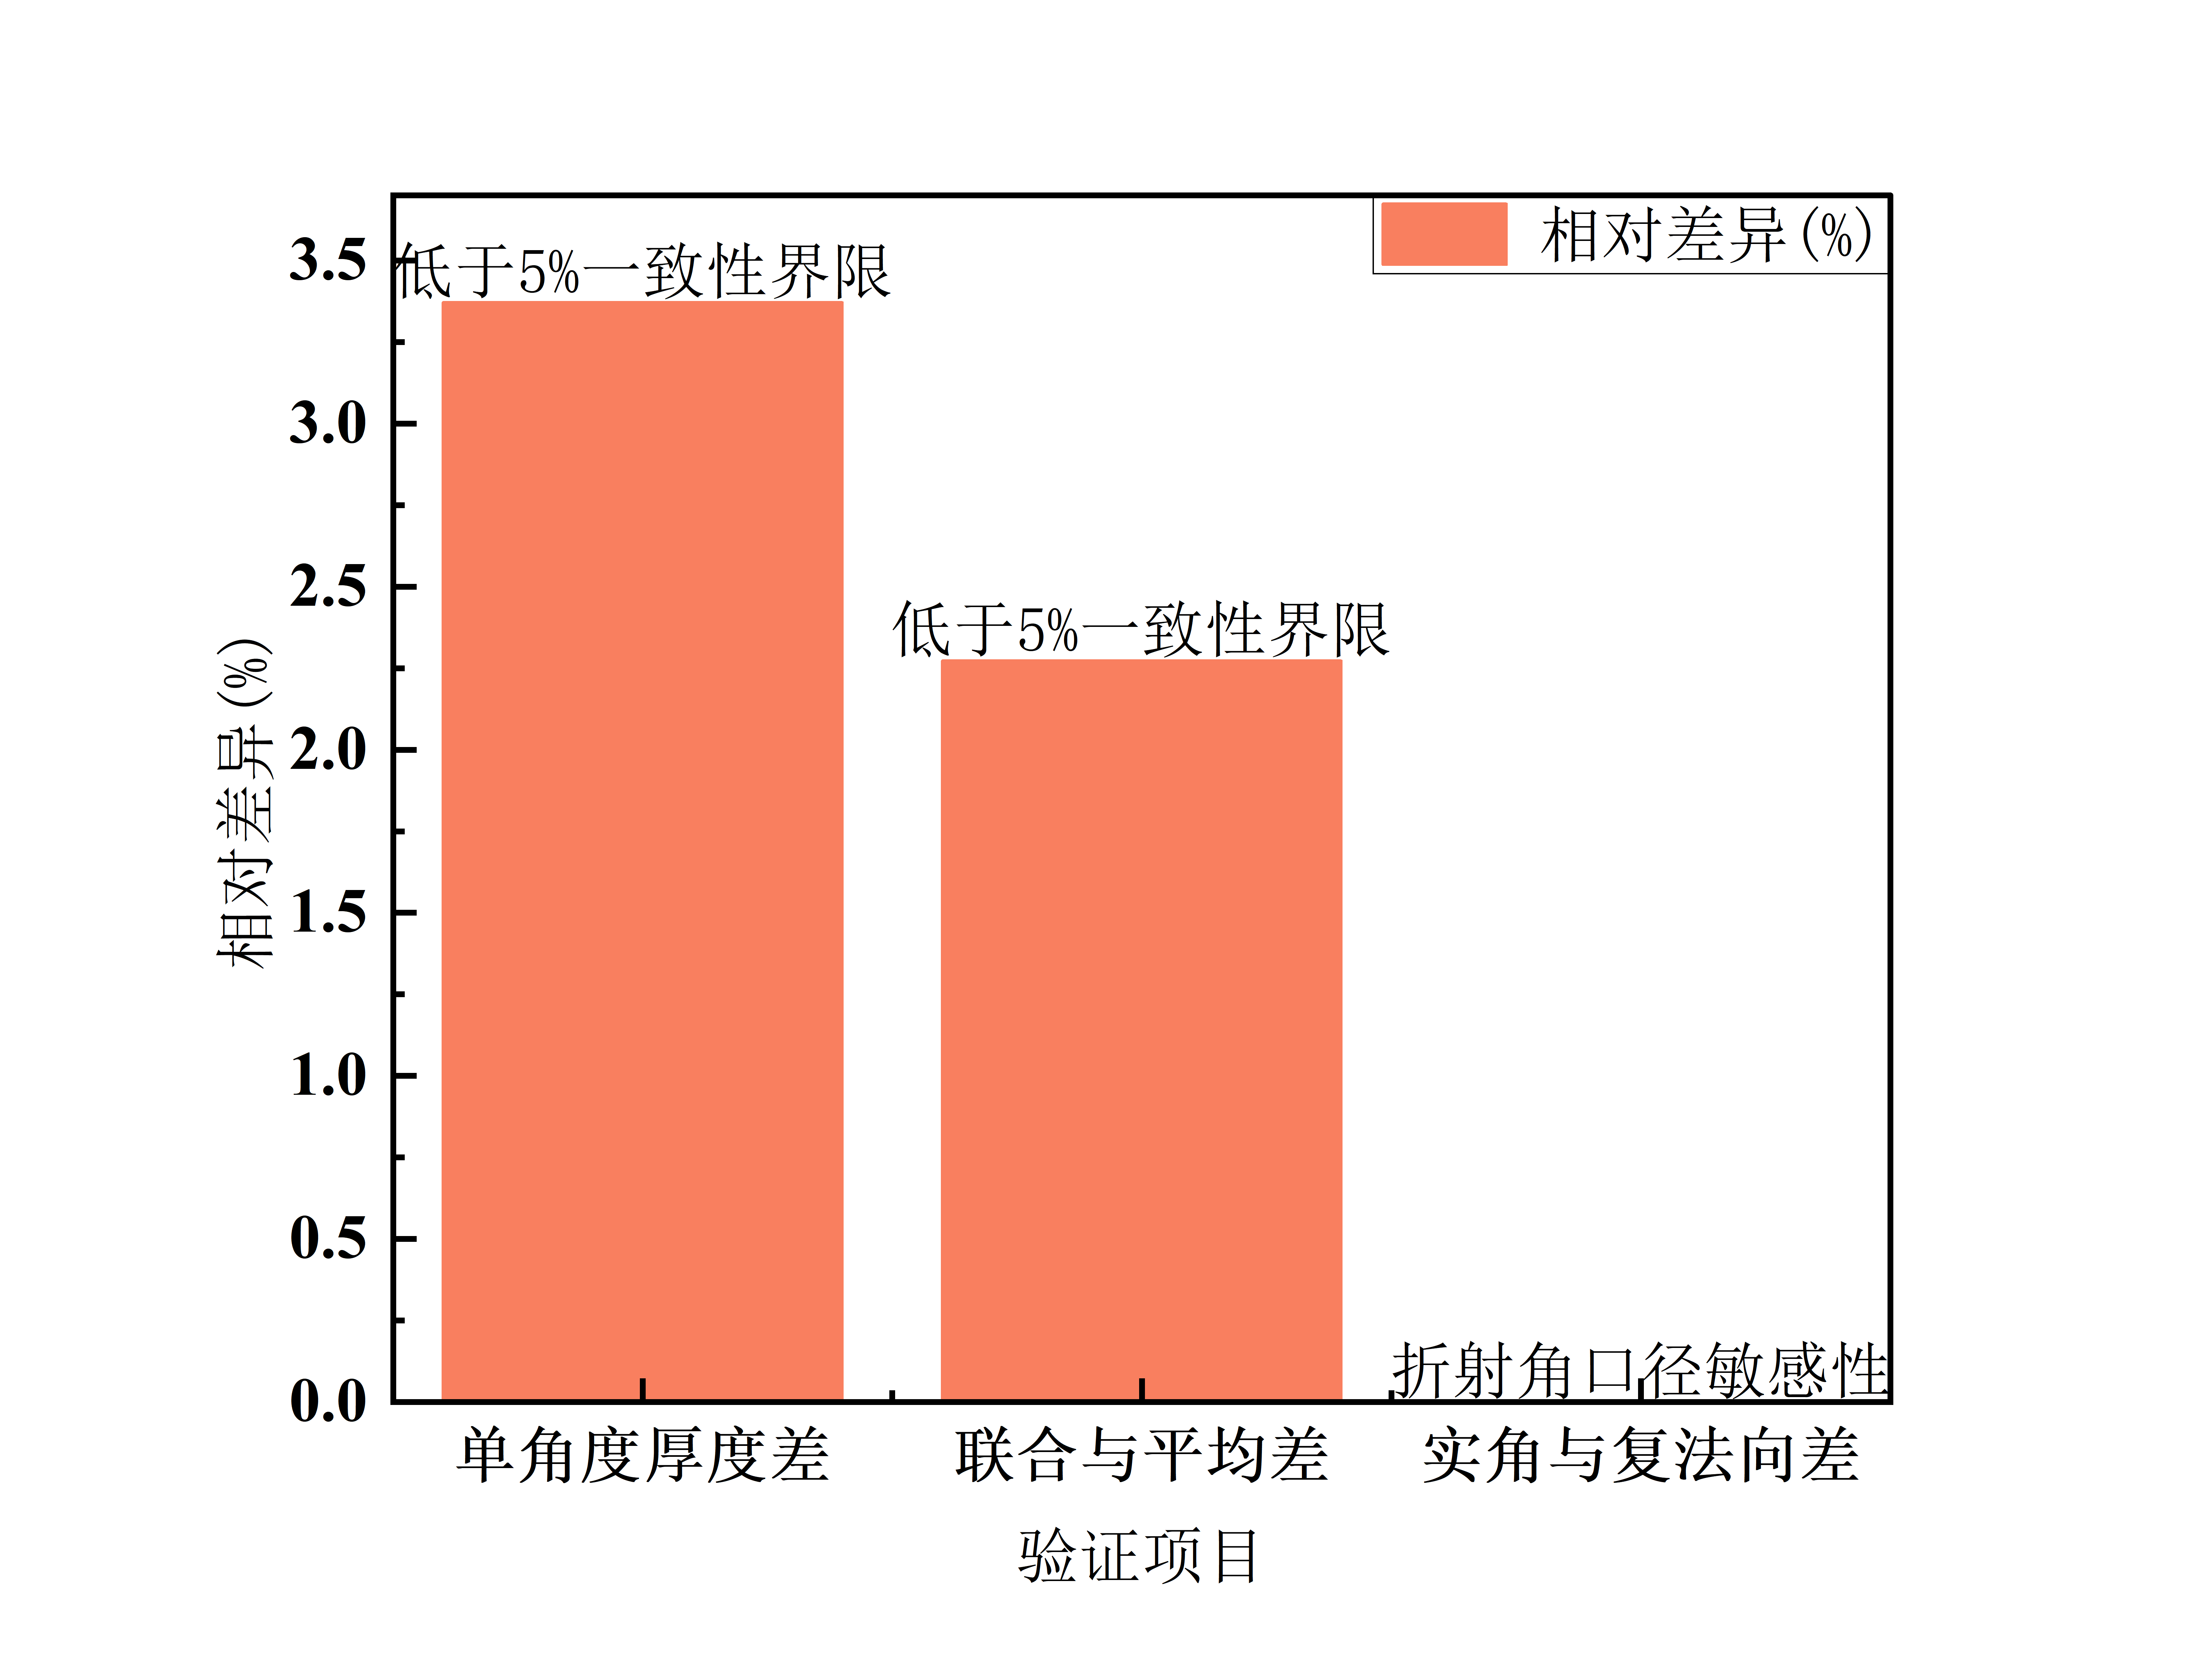
\includegraphics[width=\textwidth]{24_Si验证偏差.png}
			\caption{验证偏差分析}
			\label{fig:si_validation_bias}
		\end{subfigure}
		\caption{多初值局部盆地分析与验证偏差}
		\label{fig:si_basin_validation}
	\end{figure}
	
	\subsection{SiC回溯检验}
	
	从问题二新结果文件读取 $d_{\mathrm{SiC}}=7.7398\ \mu\mathrm{m}$，并使用两个角度各自的Sellmeier-Drude拟合参数，在 $2500\sim3300\ \mathrm{cm^{-1}}$ 计算第三束光强比。最大值分别为 $4.85\times10^{-7}\%$ 和 $4.66\times10^{-7}\%$，远小于 $0.1\%$，故高阶光束可忽略，保留
	\begin{equation}
		\boxed{d_{\mathrm{SiC}} = 7.7398\ \mu\mathrm{m}.}
	\end{equation}
	
	多初值解在同一干涉级次收敛，传播因子最大模小于1，且SiC回溯形成Q1-Q2-Q3闭环。但硅的碰撞率或载流子浓度在部分角度达到边界，说明附属参数可辨识性不足；$0.1\%$ 为工程阈值，题目未提供光源相干长度和界面粗糙度。本文仅解释厚度与高阶光束量级，不把边界处的载流子参数作为材料测量结论。
	
	\section{模型总结与评价}
	
	\subsection{模型总结}
	
	三问使用同一组单位约定和Fresnel界面系数。问题一给出双光束正演关系；问题二在弱吸收波段独立反演两个角度并取平均，得到SiC厚度 $7.7398\ \mu\mathrm{m}$；问题三以Airy公式处理硅的吸收与高阶反射，得到Si厚度 $3.2178\ \mu\mathrm{m}$，并用第三束光强比确认SiC结果无需修正。
	
	\subsection{模型优点}
	
	\begin{enumerate}
		\item 物理口径一致。带符号Fresnel系数直接包含界面反射相变，传播相位中的 $10^{-4}$ 缩放与厚度单位逐项核对，避免重复加入半波损失。
		\item 计算路线可复现。四个附件由统一读取程序载入，波段、边界、多初值方案、角度平均规则和结果文件哈希均已登记。
		\item 参数数量受到约束。硅模型固定双振子背景和有效质量，只拟合四个直接参与光谱反演的参数；即使结果与范文相差 $5.85\%$，也不释放弱可辨识量来追求数值贴合。
		\item 跨问检验明确。问题三读取问题二冻结结果及其哈希，再计算SiC第三束光强比，使“是否修正厚度”具有可重复的数值依据。
		\item 诊断图表完备。本文针对SiC提供了14张诊断图表（原始光谱、拟合对比、残差分布、多指标柱状图、多初值稳定性散点、残差ECDF等），针对硅模型提供了8张诊断图表（拟合曲线、残差热力图、厚度一致性棒棒糖图、综合指标雷达图、参数可辨识性气泡图、残差箱线图、收敛盆地气泡图和验证偏差分析），系统论证了厚度结果的可靠性与模型局限性。
	\end{enumerate}
	
	\subsection{模型局限}
	
	两个角度仍采用独立拟合，角度间差异只能用半极差描述；硅的载流子浓度或碰撞率在个别拟合中接近边界，不能作为材料参数测量值。题目未给出光源相干长度、界面粗糙度和独立椭偏数据，因此模型尚不能区分这些因素与折射率背景误差。
	
	\subsection{改进方向}
	
	若增加偏振分辨光谱或独立折射率测量，可在不释放全部背景参数的条件下增加带实验先验的校正量。若取得晶圆多位置数据，可把当前单点厚度反演扩展为厚度分布估计，并分别报告位置离散和光谱拟合误差。
	
	\newpage
	\begin{thebibliography}{99}
		\bibitem{problem} 全国大学生数学建模竞赛组委会. 2025年全国大学生数学建模竞赛B题：碳化硅外延层厚度的确定, 2025.
		\bibitem{sellmeier} Sellmeier W. Zur Erklärung der abnormen Farbenfolge im Spectrum einiger Substanzen[J]. Annalen der Physik und Chemie, 1871, 219(6): 272--282.
		\bibitem{drude} Drude P. Zur Elektronentheorie der Metalle[J]. Annalen der Physik, 1900, 306(3): 566--613.
		\bibitem{fresnel} Fresnel A. Mémoire sur la loi des modifications que la réflexion imprime à la lumière polarisée[J]. Mémoires de l'Académie des Sciences, 1823, 11: 393--433.
		\bibitem{born} Born M, Wolf E. Principles of Optics[M]. 7th ed. Cambridge: Cambridge University Press, 1999.
		\bibitem{marquardt} Marquardt D W. An algorithm for least-squares estimation of nonlinear parameters[J]. Journal of the Society for Industrial and Applied Mathematics, 1963, 11(2): 431--441.
		\bibitem{airy} Airy G B. On the intensity of light in the neighbourhood of a caustic[J]. Transactions of the Cambridge Philosophical Society, 1838, 6: 379--402.
	\end{thebibliography}
	
	% ====================== 附录：程序代码 ======================
	\newpage
	\section*{附录：程序代码}
	\addcontentsline{toc}{section}{附录：程序代码}
	
	
	
	\newpage
	\section*{AI使用报告}
	\addcontentsline{toc}{section}{AI使用报告}
	
	本项目使用生成式人工智能辅助整理资料索引、检查文件结构、实现数值程序、生成LaTeX模块和压缩语言。赛题任务、两篇参考论文和团队既有方案均由成员逐项核对；正文公式根据所选模型重新推导，全部数值由本项目程序读取官方附件后重新计算。
	
	人工智能没有替代人工决策。模型来源、参数口径、跨问依赖和结果哈希均保存在项目登记表中；问题三与范文相差 $5.85\%$ 时，团队选择保留固定背景参数的四参数重算值，并在正文披露差异。参考论文的原文、图表、代码和结果未直接拼接进本文。
	
\end{document}